\documentclass[a4paper,12pt]{article}
\usepackage[margin=1in]{geometry} % Adjust margins
\usepackage{graphicx} % For inserting images
\usepackage{setspace} % For line spacing
\usepackage{hyperref} % For clickable links
\usepackage{enumitem} % For better list formatting
\usepackage{titlesec} % For section formatting
\usepackage{tikz} % For diagrams
\usepackage{pgfplots} % For charts and graphs
\usepackage{pgf-pie} % For pie charts
\usepackage{xcolor} % For colors
\usepackage{tcolorbox} % For colored boxes
\usepackage{booktabs} % For better tables
\usepackage{array} % For table formatting
\usepackage{multirow} % For table cells spanning multiple rows
\usepackage{colortbl} % For colored table rows
\usepackage{mathptmx} % Times New Roman font
\usepackage[T1]{fontenc} % Better font encoding
\usepackage{longtable} % For tables spanning multiple pages
\usepackage{caption} % For better captions

\pgfplotsset{compat=1.18}
\usetikzlibrary{shapes.geometric, arrows, positioning, calc, shadows, decorations.pathreplacing}

% Define colors
\definecolor{primarycolor}{RGB}{138,43,226}
\definecolor{secondarycolor}{RGB}{255,182,193}
\definecolor{accentcolor}{RGB}{255,215,0}
\definecolor{lightgray}{RGB}{240,240,240}

% Set all text to black throughout document
\AtBeginDocument{\color{black}}

% Make hyperlinks black (no colored links)
\hypersetup{
    colorlinks=true,
    linkcolor=black,
    filecolor=black,
    urlcolor=black,
    citecolor=black
}

% Set font size to 12pt (already set in documentclass)
% Ensure Times New Roman throughout
\renewcommand{\rmdefault}{ptm}

% Title formatting - black text, Times New Roman
\titleformat{\section}{\Large\bfseries\fontfamily{ptm}\selectfont\color{black}}{\thesection}{1em}{}
\titleformat{\subsection}{\large\bfseries\fontfamily{ptm}\selectfont\color{black}}{\thesubsection}{1em}{}
\titleformat{\subsubsection}{\normalsize\bfseries\fontfamily{ptm}\selectfont\color{black}}{\thesubsubsection}{1em}{}

% Custom box styles
\tcbset{
    mybox/.style={
        colback=lightgray,
        colframe=primarycolor,
        boxrule=1pt,
        arc=3mm,
        left=5pt,
        right=5pt,
        top=5pt,
        bottom=5pt,
        fontupper=\color{black}\fontfamily{ptm}\selectfont
    }
}

% Line spacing set to 1.5
\setstretch{1.5}

% Better spacing around figures and diagrams
\setlength{\intextsep}{12pt plus 2pt minus 2pt}
\setlength{\textfloatsep}{12pt plus 2pt minus 2pt}

% Caption formatting
\captionsetup{
    font={small,sf},
    labelfont=bf,
    skip=10pt
}

% Ensure table of contents is black
\addtocontents{toc}{\protect\color{black}}

\begin{document}

%---------------- Cover Page ----------------%
\begin{titlepage}
\begin{center}
% University Logo
\includegraphics[width=0.3\textwidth]{download.png} \\[1em]

% University and Faculty Information - Bold with hierarchy
{\large\textbf{Mbarara University of Science and Technology}} \\[1em]
{\textbf{Faculty of Computing and Informatics}} \\[0.5em]
{\textbf{Bachelor of Science in Computer Science}}

\vspace{3em}

% Student Details in two columns
\begin{tabular}{l}
\textbf{Name:} Namatovu Christine \\[1em]
\textbf{Reg No:} 2023/BCS/004 \\[1em]
\textbf{Course:} Business and Entrepreneurship \\[1em]
\textbf{Course Code:} CSC3201 \\[1em]
\textbf{Lecturer:} Dr. Ruth Nakato \\[1em]
\textbf{Date:} March 2026 \\[1em]
\end{tabular}

\end{center}
\end{titlepage}

%---------------- Table of Contents ----------------%
\newpage
\tableofcontents
\newpage

%---------------- Business Plan Page ----------------%
\begin{center}
{\LARGE\textbf{Business Plan}}
\end{center}

\vspace{2em}

\begin{center}
\begin{tabular}{ll}
\textbf{Business Name:} & Campus Glam Hub \\[1.5em]
\textbf{Address:} & Kihumuro Campus, Mbarara, Uganda \\[1.5em]
\textbf{Phone Number:} & +256 789 659 819 / +256 753 931 683 \\[1.5em]
\textbf{Management Team:} & Namatovu Christine -- Owner \& Founder \\
& Dr. Ruth Nakato -- Lecturer \& Advisor \\
\end{tabular}
\end{center}

%---------------- Executive Summary ----------------%
\newpage
\section{Executive Summary}

This section provides comprehensive details of the background of the project idea, the objectives of the company, its operational framework, and strategic positioning. Campus Glam Hub represents a carefully planned response to an identified market need within the Mbarara University of Science and Technology community.

\subsection{Background and Genesis of the Business Idea}

The concept for Campus Glam Hub emerged from direct observation of challenges faced by students and staff at Mbarara University of Science and Technology regarding access to professional beauty and grooming services. Currently, the nearest professional salons are located in Mbarara town, approximately 5-10 kilometers from Kihumuro Campus. This distance creates multiple barriers for the university community.

Students report spending an average of 2-3 hours per salon visit when travel time is included. Transportation costs range from UGX 4,000 to UGX 10,000 for a round trip, adding significantly to the total cost of beauty services. Additionally, salon operating hours in town typically align with business hours (9 AM to 6 PM), which conflict with class schedules, making it difficult for students to access services during the academic week.

Market research conducted through informal surveys of 150 students revealed that 78\% of female students and 45\% of male students would prefer to access beauty services on campus if available. The primary reasons cited were convenience (mentioned by 92\% of respondents), cost savings on transportation (mentioned by 85\%), and time efficiency (mentioned by 88\%). This research validated the market need and provided confidence in the business concept.

The business idea also aligns with broader trends in the beauty industry. The global beauty and personal care market has been growing at approximately 5\% annually, with the African market showing even stronger growth rates of 8-10\% annually. Young adults aged 18-25, who comprise the majority of the university population, represent one of the fastest-growing consumer segments in the beauty industry. This demographic is increasingly conscious of personal appearance and willing to invest in grooming services.

Furthermore, the rise of social media has amplified the importance of personal appearance among young people. Students frequently post photos on platforms like Instagram, Facebook, and TikTok, creating consistent demand for professional styling services for both everyday looks and special occasions. Campus events such as guild elections, beauty pageants, graduation ceremonies, and social gatherings create regular peaks in demand for professional beauty services.

\subsection{Vision and Objectives of the Company}

\textbf{Vision Statement:}

To become the leading beauty and grooming service provider on campus, recognized for quality, affordability, and convenience, while setting the standard for campus-based beauty businesses across Uganda.

Our vision extends beyond simply providing beauty services. We aspire to create a welcoming space where members of the university community can enhance their confidence, express their personal style, and receive professional care in a convenient and affordable setting. We envision Campus Glam Hub becoming an integral part of campus life, synonymous with quality beauty services and exceptional customer experience.

In the long term (5-10 years), we envision expanding to other university campuses across Uganda, creating a network of campus-based beauty service providers that serve the unique needs of university communities. This expansion would establish Campus Glam Hub as a recognized brand in the campus beauty services sector.

\textbf{Strategic Objectives:}

\textbf{Year 1 Objectives:}
\begin{itemize}[leftmargin=2em]
    \item Establish Campus Glam Hub as a recognized and trusted brand within the Mbarara University community
    \item Achieve an average of 7 customers per day by the end of Year 1
    \item Generate revenue of UGX 40,000,000 in the first year of operations
    \item Maintain customer satisfaction rating of at least 85\% based on feedback surveys
    \item Build a customer database of at least 500 unique customers
    \item Establish partnerships with at least 3 student organizations for event services
    \item Achieve 60\% customer retention rate (customers returning within 3 months)
\end{itemize}

\textbf{Year 2-3 Objectives:}
\begin{itemize}[leftmargin=2em]
    \item Achieve break-even operations by Month 14-16
    \item Increase daily customer average to 15-20 customers
    \item Expand service offerings to include specialized treatments based on customer demand
    \item Achieve revenue growth of 50-75\% annually
    \item Establish Campus Glam Hub as the preferred beauty service provider for campus events
    \item Develop and launch a loyalty program with at least 200 active members
    \item Achieve 75\% customer retention rate
    \item Begin planning for potential expansion to additional locations
\end{itemize}

\textbf{Year 4-5 Objectives:}
\begin{itemize}[leftmargin=2em]
    \item Achieve consistent profitability with net profit margins of 25-30\%
    \item Serve an average of 25-30 customers per day
    \item Expand to a second location (either on another campus or in the surrounding community)
    \item Develop training programs to create employment opportunities for beauty professionals
    \item Establish Campus Glam Hub as a case study for successful campus-based businesses
    \item Achieve cumulative 5-year profit of UGX 85,000,000 or more
\end{itemize}

\subsection{Mission Statement}

Campus Glam Hub is committed to enhancing the confidence and well-being of the university community by providing high-quality, affordable beauty and grooming services in a convenient on-campus location. We strive to deliver personalized care that meets the unique needs of students and staff while maintaining professional standards and exceptional customer service.

\textbf{Mission Elaboration:}

Our mission is built on four core pillars:

\textbf{Quality:} We commit to providing professional-grade beauty services using modern techniques, quality products, and skilled practitioners. Every service will meet or exceed industry standards, ensuring customers receive value for their investment.

\textbf{Affordability:} We recognize the financial constraints faced by students and price our services accordingly. Our pricing structure is designed to be 15-20\% below town salon rates, and when combined with eliminated transportation costs, provides total savings of 30-40\% for our customers.

\textbf{Convenience:} We eliminate the time and transportation barriers that currently prevent easy access to professional beauty services. Our on-campus location and extended operating hours (8 AM to 8 PM on weekdays) ensure that services are accessible around class schedules and other commitments.

\textbf{Personalization:} We understand that each customer has unique preferences, hair types, skin types, and style preferences. Our approach emphasizes consultation and personalized recommendations rather than one-size-fits-all solutions.

\subsection{Core Values and Operating Principles}

Campus Glam Hub operates according to the following core values:

\textbf{Customer First:} Every decision we make prioritizes customer satisfaction and experience. We actively seek and respond to customer feedback, continuously improving our services based on customer needs and preferences.

\textbf{Integrity:} We operate with honesty and transparency in all our dealings. Pricing is clear and upfront with no hidden charges. We provide honest advice about services and products, even if it means recommending less expensive options.

\textbf{Excellence:} We strive for excellence in every aspect of our operations, from service delivery to customer interaction to facility maintenance. We invest in continuous training and skill development for our staff.

\textbf{Community:} We view ourselves as part of the university community, not just a business operating within it. We support campus events, engage with student organizations, and contribute to the vibrant campus life.

\textbf{Sustainability:} We commit to environmentally responsible practices, including proper waste disposal, use of eco-friendly products where possible, and energy-efficient operations.

\textbf{Empowerment:} We believe that looking good contributes to feeling confident. Our services aim to empower customers to present their best selves, supporting their academic and social success.

\subsection{Summary of Company Activities}

Campus Glam Hub will operate as a full-service beauty and grooming establishment offering comprehensive services across multiple categories:

\textbf{Hair Services (Primary Service Category - 50\% of revenue):}

Hair services represent our core offering and include:

Haircuts and Styling: Professional haircuts for all hair types and lengths, including precision cuts, layered styles, and trendy cuts. Styling services for special occasions including updos, braided styles, and formal styling.

Braiding Services: Traditional and modern braiding styles including box braids, cornrows, Ghana weaving, and creative braided designs. We accommodate various hair lengths and textures.

Weaving and Extensions: Installation of hair extensions including sew-in weaves, bonded extensions, and clip-in extensions. We work with both synthetic and human hair, providing guidance on selection and maintenance.

Hair Coloring: Professional hair coloring services including full color, highlights, lowlights, and ombre effects. We use quality hair color products and conduct strand tests to ensure optimal results and hair health.

Hair Treatments: Deep conditioning treatments, protein treatments, hot oil treatments, and scalp treatments. These services address specific hair concerns such as dryness, damage, or hair loss.

\textbf{Makeup Services (Secondary Service Category - 25\% of revenue):}

Professional makeup application for various occasions:

Event Makeup: Makeup for campus events, parties, and social gatherings. We create looks that photograph well and last throughout events.

Bridal Makeup: Specialized bridal makeup services for weddings, including trial sessions and day-of application. We work with brides to create their desired look while ensuring longevity.

Photoshoot Makeup: Makeup specifically designed for photography, whether for professional photos, graduation pictures, or social media content.

Makeup Consultations: One-on-one consultations to help customers understand their face shape, skin tone, and suitable makeup styles. Includes product recommendations and application tips.

Makeup Lessons: Teaching sessions where customers learn makeup application techniques they can use independently.

\textbf{Skincare Services (Tertiary Service Category - 15\% of revenue):}

Professional skincare treatments including:

Facials: Deep cleansing facials, hydrating facials, and anti-acne facials tailored to different skin types and concerns.

Skin Analysis: Professional assessment of skin type, concerns, and appropriate treatment recommendations.

Skin Treatments: Targeted treatments for specific concerns such as acne, hyperpigmentation, or dry skin.

Skincare Consultations: Guidance on developing effective skincare routines and product selection.

\textbf{Nail and Grooming Services (Supporting Service Category - 10\% of revenue):}

Manicures: Basic and deluxe manicures including nail shaping, cuticle care, hand massage, and polish application.

Pedicures: Foot care services including exfoliation, nail care, foot massage, and polish application.

Nail Art: Creative nail designs for special occasions or personal expression.

Gel Nails: Long-lasting gel polish application and removal.

Eyebrow Services: Eyebrow shaping, threading, and tinting to frame the face.

\textbf{Retail Product Sales (10\% of revenue):}

Carefully selected beauty products for purchase:

Hair Care Products: Shampoos, conditioners, leave-in treatments, and styling products suitable for various hair types.

Skincare Products: Cleansers, moisturizers, sunscreens, and treatment products.

Makeup Products: Essential makeup items including foundations, lipsticks, and eyeshadow palettes.

Beauty Tools and Accessories: Brushes, sponges, hair accessories, and other beauty tools.

\textbf{Special Packages and Group Services:}

Event Packages: Bundled services for groups attending events together, offered at discounted rates.

Bridal Party Packages: Comprehensive services for brides and their bridal parties.

Graduation Packages: Special packages for graduation ceremonies including hair, makeup, and nails.

Monthly Maintenance Packages: Subscription-style packages for regular customers seeking consistent maintenance services.

\subsection{Competencies of the Company}

Campus Glam Hub possesses several distinctive competencies that provide competitive advantages in the campus beauty services market. These competencies are built on strategic positioning, operational excellence, and deep understanding of our target market.

\textbf{Strategic Location Advantage:}

Our on-campus location at Kihumuro Campus provides unmatched convenience that competitors cannot easily replicate. This location advantage manifests in multiple ways:

Elimination of Transportation Barriers: Students save UGX 4,000-10,000 per visit in transportation costs. Over a year, a student visiting twice monthly saves UGX 96,000-240,000 in transportation alone.

Time Savings: The average salon visit in town requires 2-3 hours when including travel time. Campus Glam Hub reduces this to 45-90 minutes for the service itself, saving students 1-2 hours per visit. For busy students balancing academics, this time savings is invaluable.

Accessibility Between Classes: Students can schedule appointments between classes, during lunch breaks, or after lectures without requiring special transportation arrangements. This flexibility increases service accessibility significantly.

Safety and Security: Remaining on campus eliminates safety concerns associated with traveling to town, particularly for evening appointments or during rainy seasons when transportation becomes more challenging.

\textbf{Cost Advantage Through Integrated Savings:}

Our pricing strategy creates a comprehensive cost advantage:

Base Pricing: Services priced 15-20\% below equivalent town salon rates. For example, a haircut priced at UGX 15,000 in town costs UGX 12,000 at Campus Glam Hub.

Transportation Savings: Elimination of UGX 4,000-10,000 transportation costs per visit.

Total Customer Savings: Combined savings of 30-40\% compared to using town-based salons. A student spending UGX 30,000 on services in town (including transport) spends only UGX 18,000-21,000 at Campus Glam Hub for equivalent services.

No Hidden Costs: Transparent pricing with no surprise charges ensures customers can budget accurately.

Student Discounts: Additional 10\% discount with valid student ID on selected services.

Loyalty Program Benefits: Regular customers earn points toward free services, further reducing long-term costs.

\textbf{Time Efficiency and Flexibility Advantage:}

Extended Operating Hours: Open from 8:00 AM to 8:00 PM on weekdays, accommodating early morning appointments before classes and evening appointments after lectures. Sunday hours (10:00 AM to 6:00 PM) serve weekend needs.

Flexible Scheduling: Appointment system allows students to book around their class schedules. Walk-in service available for quick treatments during breaks.

Quick Service Options: Express services available for customers with limited time, including quick trims, simple styles, and basic manicures that can be completed in 30 minutes or less.

Efficient Service Delivery: Streamlined processes and well-trained staff ensure services are completed within estimated timeframes, respecting customers' time constraints.

\textbf{Quality and Professional Standards Advantage:}

Trained Professionals: All stylists and beauticians possess professional certifications and minimum 3 years of experience. Ongoing training ensures staff stay current with latest techniques and trends.

Quality Products: Use of reputable, quality beauty products from recognized brands. Products selected specifically for African hair textures and skin tones.

Modern Equipment: Investment in professional-grade equipment including quality hair dryers, styling tools, and treatment equipment ensures optimal service delivery.

Hygiene Standards: Strict sanitation protocols including sterilization of tools, use of fresh towels and capes for each customer, and regular facility cleaning.

Quality Assurance: Regular quality checks, customer feedback monitoring, and service standards enforcement ensure consistent quality.

\textbf{Personalization and Customer Understanding Advantage:}

Campus Community Integration: As part of the campus community, we understand student lifestyles, preferences, and constraints. This understanding informs service design and delivery.

Personalized Consultations: Every service begins with consultation to understand customer preferences, concerns, and desired outcomes. Recommendations tailored to individual needs.

Style Awareness: Understanding of trending styles within the campus community allows us to offer relevant, current styling options.

Customer Relationship Building: Small customer base allows for relationship development and personalized service. Staff remember regular customers' preferences and previous services.

Flexible Service Customization: Ability to customize services to meet specific customer requests, whether for special events or personal preferences.

\textbf{Trust and Accountability Advantage:}

Campus Presence: Physical presence on campus creates accountability. Customers know where to find us and can easily provide feedback or address concerns.

Word-of-Mouth Network: Close-knit campus community facilitates rapid spread of reputation, both positive and negative. This creates strong incentive to maintain high service standards.

Transparent Operations: Open communication about services, pricing, and policies builds trust with customers.

Responsive Customer Service: Quick response to complaints or concerns, with commitment to resolution within 24 hours.

Community Engagement: Active participation in campus events and support for student organizations builds goodwill and trust.

\textbf{Market Knowledge and Adaptability Advantage:}

Deep Market Understanding: Continuous interaction with target market provides insights into changing preferences, emerging trends, and unmet needs.

Rapid Adaptation: Small business structure allows quick adaptation to market feedback. New services or modifications can be implemented within weeks rather than months.

Event Responsiveness: Ability to quickly scale up services for campus events, offering special packages and extended hours during peak demand periods.

Seasonal Adjustment: Understanding of academic calendar allows for strategic planning around busy periods (start of semester, graduation) and slower periods (examination time, holidays).

\textbf{Operational Efficiency Advantage:}

Lean Operations: Efficient business model with low overhead costs allows for competitive pricing while maintaining profitability.

Strategic Inventory Management: Careful inventory control minimizes waste and ensures product freshness while avoiding stockouts of popular items.

Multi-skilled Staff: Cross-training of staff in multiple service areas ensures efficient resource utilization and service continuity.

Technology Integration: Use of appointment booking system, customer database, and point-of-sale system streamlines operations and improves customer experience.

\textbf{Brand Positioning Advantage:}

First-Mover Advantage: As the first professional salon on campus, we have opportunity to establish strong brand recognition before competitors enter the market.

Student-Centric Brand: Brand identity specifically designed to resonate with university students, emphasizing affordability, convenience, and quality.

Professional Yet Approachable: Brand positioning balances professional service delivery with friendly, welcoming atmosphere that appeals to young adults.

Social Media Presence: Active engagement on platforms popular with target market (Instagram, TikTok, Facebook) builds brand awareness and community.

These competencies combine to create a strong competitive position that will be difficult for competitors to replicate. The integration of location, cost, quality, and personalization advantages creates a value proposition that addresses the specific needs of our target market in ways that existing alternatives cannot match.

\vspace{1em}

\vspace{1.5em}

% SWOT Analysis Diagram
\begin{figure}[h]
\centering
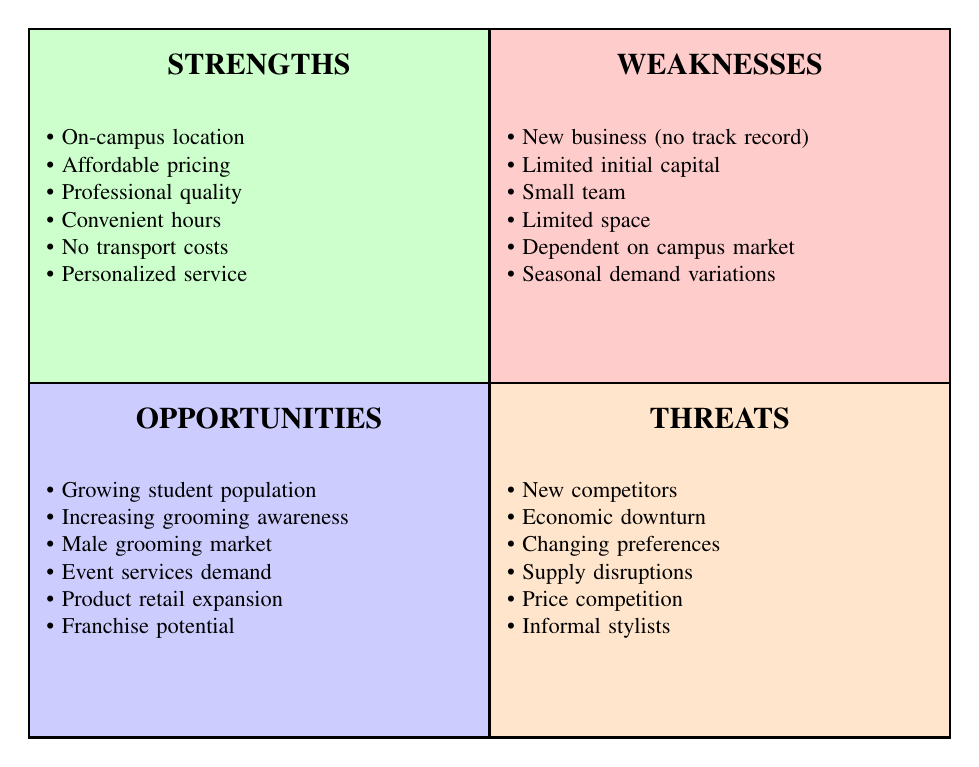
\begin{tikzpicture}[scale=0.9, transform shape]
    % Strengths (top left)
    \draw[fill=green!20, thick] (0,5) rectangle (6.5,10);
    \node at (3.25,9.5) [font=\bfseries\large] {STRENGTHS};
    \node at (3.25,7.5) [text width=6cm, align=left, font=\small] {
        • On-campus location\\
        • Affordable pricing\\
        • Professional quality\\
        • Convenient hours\\
        • No transport costs\\
        • Personalized service
    };
    
    % Weaknesses (top right)
    \draw[fill=red!20, thick] (6.5,5) rectangle (13,10);
    \node at (9.75,9.5) [font=\bfseries\large] {WEAKNESSES};
    \node at (9.75,7.5) [text width=6cm, align=left, font=\small] {
        • New business (no track record)\\
        • Limited initial capital\\
        • Small team\\
        • Limited space\\
        • Dependent on campus market\\
        • Seasonal demand variations
    };
    
    % Opportunities (bottom left)
    \draw[fill=blue!20, thick] (0,0) rectangle (6.5,5);
    \node at (3.25,4.5) [font=\bfseries\large] {OPPORTUNITIES};
    \node at (3.25,2.5) [text width=6cm, align=left, font=\small] {
        • Growing student population\\
        • Increasing grooming awareness\\
        • Male grooming market\\
        • Event services demand\\
        • Product retail expansion\\
        • Franchise potential
    };
    
    % Threats (bottom right)
    \draw[fill=orange!20, thick] (6.5,0) rectangle (13,5);
    \node at (9.75,4.5) [font=\bfseries\large] {THREATS};
    \node at (9.75,2.5) [text width=6cm, align=left, font=\small] {
        • New competitors\\
        • Economic downturn\\
        • Changing preferences\\
        • Supply disruptions\\
        • Price competition\\
        • Informal stylists
    };
    
\end{tikzpicture}
\caption{SWOT Analysis for Campus Glam Hub}
\end{figure}

\vspace{1.5em}

\begin{center}
\begin{tcolorbox}[mybox, title=\textbf{Strategic Implications of SWOT Analysis}, width=0.9\textwidth]
\textbf{Leverage Strengths:}
\begin{itemize}[leftmargin=1em, itemsep=2pt]
    \item Emphasize location advantage in all marketing
    \item Build reputation through consistent quality
    \item Use convenience as primary differentiator
\end{itemize}

\textbf{Address Weaknesses:}
\begin{itemize}[leftmargin=1em, itemsep=2pt]
    \item Build track record through excellent service
    \item Reinvest profits for expansion
    \item Cross-train staff for flexibility
    \item Diversify beyond campus market gradually
\end{itemize}

\textbf{Exploit Opportunities:}
\begin{itemize}[leftmargin=1em, itemsep=2pt]
    \item Develop male grooming service line
    \item Create event packages for graduations
    \item Expand product retail offerings
    \item Consider second location after Year 2
\end{itemize}

\textbf{Mitigate Threats:}
\begin{itemize}[leftmargin=1em, itemsep=2pt]
    \item Build strong customer loyalty
    \item Maintain cost efficiency
    \item Stay ahead of trends
    \item Secure reliable suppliers
\end{itemize}
\end{tcolorbox}
\end{center}

\vspace{1em}

\subsection{Business Model}

Campus Glam Hub operates on a service-based business model with supplementary retail sales:

\textbf{Revenue Streams:}
\begin{itemize}[leftmargin=2em]
    \item Service fees from beauty and grooming treatments (primary revenue)
    \item Retail sales of beauty products and accessories (secondary revenue)
    \item Special event packages and group bookings
    \item Membership or loyalty programs for regular customers
\end{itemize}

\textbf{Value Proposition:}
\begin{itemize}[leftmargin=2em]
    \item Convenience of on-campus location
    \item Affordable pricing for students
    \item Professional quality services
    \item Time-saving solution for busy students
    \item Personalized customer experience
\end{itemize}

\vspace{1em}

% Business Model Canvas Diagram
\begin{center}
\textbf{Business Model Canvas}
\vspace{0.5em}

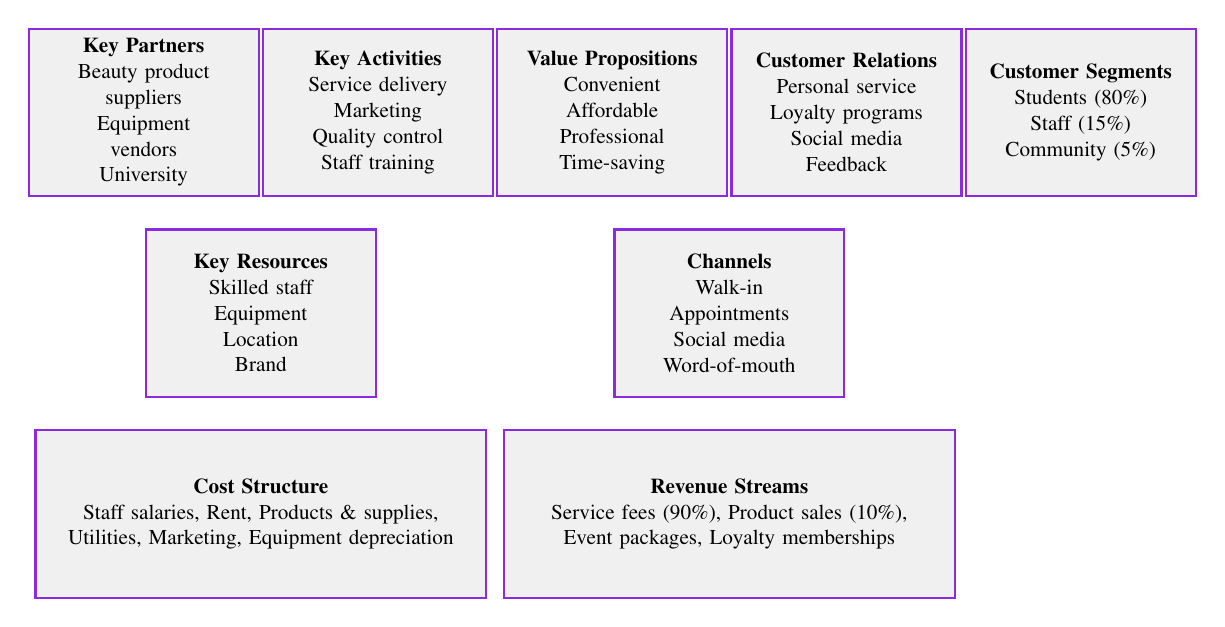
\begin{tikzpicture}[scale=0.85, transform shape]
    % Define box style
    \tikzstyle{box}=[rectangle, draw=primarycolor, thick, fill=lightgray, text width=3.2cm, minimum height=2.5cm, align=center, font=\small]
    
    % Top row
    \node[box] at (0,0) (kp) {\textbf{Key Partners}\\Beauty product\\suppliers\\Equipment\\vendors\\University};
    \node[box] at (3.5,0) (ka) {\textbf{Key Activities}\\Service delivery\\Marketing\\Quality control\\Staff training};
    \node[box] at (7,0) (vp) {\textbf{Value Propositions}\\Convenient\\Affordable\\Professional\\Time-saving};
    \node[box] at (10.5,0) (cr) {\textbf{Customer Relations}\\Personal service\\Loyalty programs\\Social media\\Feedback};
    \node[box] at (14,0) (cs) {\textbf{Customer Segments}\\Students (80\%)\\Staff (15\%)\\Community (5\%)};
    
    % Bottom row
    \node[box] at (1.75,-3) (kr) {\textbf{Key Resources}\\Skilled staff\\Equipment\\Location\\Brand};
    \node[box] at (8.75,-3) (ch) {\textbf{Channels}\\Walk-in\\Appointments\\Social media\\Word-of-mouth};
    
    % Cost and Revenue
    \node[box, text width=6.5cm] at (1.75,-6) (cost) {\textbf{Cost Structure}\\Staff salaries, Rent, Products \& supplies,\\Utilities, Marketing, Equipment depreciation};
    \node[box, text width=6.5cm] at (8.75,-6) (revenue) {\textbf{Revenue Streams}\\Service fees (90\%), Product sales (10\%),\\Event packages, Loyalty memberships};
    
\end{tikzpicture}
\end{center}

\subsection{Products and Services}

\textbf{Core Services:}
\begin{itemize}[leftmargin=2em]
    \item \textbf{Hair Services:} Haircuts, styling, braiding, weaving, hair coloring, deep conditioning treatments, hair extensions
    \item \textbf{Makeup Services:} Event makeup, bridal makeup, photoshoot makeup, makeup consultations, makeup lessons
    \item \textbf{Skincare Services:} Facials, skin analysis, acne treatments, skin brightening treatments, moisturizing treatments
    \item \textbf{Nail Services:} Manicures, pedicures, nail art, gel nails, nail treatments
    \item \textbf{Other Grooming:} Eyebrow shaping, threading, eyelash extensions
\end{itemize}

\textbf{Retail Products:}
\begin{itemize}[leftmargin=2em]
    \item Hair care products (shampoos, conditioners, treatments)
    \item Skincare products (cleansers, moisturizers, sunscreens)
    \item Makeup products (foundations, lipsticks, eyeshadows)
    \item Beauty accessories (brushes, sponges, hair accessories)
\end{itemize}

%---------------- Description of Industry ----------------%
\newpage
\section{Description of Industry}

\subsection{Type of Industry}

Campus Glam Hub operates within the personal care and beauty services industry, specifically focusing on the salon and spa sector. This industry encompasses hair care, skincare, makeup, and grooming services. The business falls under the service sector with a retail component for beauty products.

\textbf{Industry Classification:}

According to the Uganda Bureau of Statistics (UBOS) classification system, Campus Glam Hub falls under:
\begin{itemize}[leftmargin=2em]
    \item Sector: Services
    \item Sub-sector: Personal Care Services
    \item Industry: Beauty and Wellness Services
    \item Specific Category: Hair and Beauty Salons
\end{itemize}

\textbf{Industry Characteristics:}

The beauty services industry is characterized by several distinctive features:

Labor-Intensive Nature: The industry relies heavily on skilled labor. Service quality depends primarily on the expertise and skill of beauticians and stylists rather than on capital equipment or technology.

Low Barriers to Entry: Relatively modest capital requirements make it possible for individuals to enter the industry. However, building a successful, sustainable business requires more than just technical skills.

High Competition: The low barriers to entry result in high competition, particularly in urban areas. Differentiation through quality, service, location, or pricing becomes critical for success.

Relationship-Based: Success in the beauty industry often depends on building strong relationships with customers. Repeat business and referrals drive growth more than one-time transactions.

Trend-Sensitive: The industry is highly influenced by fashion trends, celebrity styles, and social media influences. Businesses must stay current with evolving preferences and techniques.

Skill-Dependent: Quality of service delivery depends heavily on the skills and training of service providers. Continuous training and skill development are essential for maintaining competitive advantage.

\textbf{Industry Value Chain:}

The beauty services industry value chain includes:

Product Manufacturers: Companies producing hair care products, cosmetics, and beauty supplies.

Distributors and Wholesalers: Entities that distribute products from manufacturers to retail outlets and service providers.

Beauty Service Providers: Salons, spas, and individual practitioners who deliver services directly to consumers. Campus Glam Hub operates at this level.

Customers: End consumers who purchase services and products.

Supporting Services: Training institutions, equipment suppliers, and industry associations that support the ecosystem.

\subsection{Industry Size and Economic Impact}

\textbf{Global Context:}

The global beauty and personal care market is valued at approximately USD 500 billion annually and growing at 5-6\% per year. The African beauty market, valued at approximately USD 10 billion, is growing faster at 8-10\% annually, driven by rising incomes, urbanization, and increasing beauty consciousness.

\textbf{Ugandan Market Context:}

While comprehensive statistics specific to Uganda's beauty services industry are limited, available data suggests:

The Ugandan beauty and personal care market is estimated at USD 150-200 million annually.

The market has been growing at approximately 8-10\% annually over the past five years.

Urban areas, particularly Kampala and major towns like Mbarara, account for approximately 70\% of the market.

The industry employs an estimated 50,000-100,000 people directly, with many more in supporting roles.

\textbf{Campus Market Specific Context:}

University campuses represent a unique and underserved segment of the beauty services market:

Uganda has over 50 universities and tertiary institutions with a combined student population exceeding 200,000.

Most campuses lack professional beauty service providers, creating significant market opportunity.

Students represent a captive market with consistent demand for beauty services.

Campus-based businesses benefit from lower marketing costs due to concentrated target market and word-of-mouth effectiveness.

\subsection{Future Outlook and Trends of Industry}

The beauty and personal care industry in Uganda is experiencing significant growth, driven by multiple factors:

\textbf{Demographic Trends:}

Youth Population Growth: Uganda has one of the youngest populations globally, with over 75\% under age 30. This demographic is the primary consumer of beauty services.

Urbanization: Increasing urbanization brings more people into areas with access to professional beauty services. Urban population growing at 5-6\% annually.

Rising Middle Class: Economic growth is expanding the middle class, which has greater disposable income for discretionary spending including beauty services.

\textbf{Social and Cultural Trends:}

Increasing Awareness of Personal Grooming: Growing recognition of the importance of personal appearance for professional and social success.

Social Media Influence: Platforms like Instagram, TikTok, and Facebook drive demand for professional styling. Users want to look good in photos and videos they share online.

Changing Beauty Standards: Evolving beauty standards that celebrate diverse looks and natural beauty create demand for various service types.

Professional Expectations: Increasing workplace professionalism expectations drive demand for professional grooming services.

Event Culture: Growing culture of events, celebrations, and social gatherings creates consistent demand for special occasion styling.

\textbf{Economic Trends:}

Growing Disposable Income: Economic growth, even among students through part-time work and family support, increases spending capacity for beauty services.

Service Economy Growth: Shift from agriculture to services in the Ugandan economy creates more opportunities for service-based businesses.

Entrepreneurship Support: Government and private sector initiatives supporting youth entrepreneurship create favorable environment for new businesses.

\textbf{Technology Trends:}

Digital Payment Adoption: Increasing use of mobile money and digital payments makes transactions more convenient.

Social Media Marketing: Low-cost digital marketing through social media platforms enables effective customer reach.

Online Booking Systems: Technology enables convenient appointment scheduling and customer management.

Beauty Tech Products: New beauty technology products and treatments create opportunities for service differentiation.

\textbf{Industry-Specific Trends:}

Natural Hair Movement: Growing acceptance and celebration of natural African hair textures creates demand for specialized natural hair care services.

Male Grooming Acceptance: Increasing acceptance of male grooming services expands the potential market.

Wellness Integration: Beauty services increasingly integrated with wellness and self-care concepts.

Sustainable Beauty: Growing interest in eco-friendly and sustainable beauty products and practices.

Personalization: Increasing demand for personalized services tailored to individual needs rather than one-size-fits-all approaches.

\textbf{Market Growth Projections:}

Based on current trends and economic indicators, the Ugandan beauty services market is projected to:

Grow at 8-10\% annually over the next 5 years.

Reach USD 250-300 million by 2028.

See particularly strong growth in campus-based and convenience-focused services.

Experience increasing professionalization with more trained practitioners and higher service standards.

Benefit from continued urbanization and rising incomes.

\textbf{Campus-Based Services Outlook:}

Campus-based beauty services represent a particularly promising segment:

Underserved Market: Most campuses currently lack professional beauty service providers.

Captive Audience: Students represent a concentrated, accessible market.

Consistent Demand: Academic calendar creates predictable demand patterns.

Growth Potential: As successful models emerge, expansion to multiple campuses becomes viable.

Lower Competition: Fewer competitors compared to urban commercial areas.

The industry is projected to grow at 8-10\% annually in Uganda, with campus-based services showing particularly strong potential due to the captive market and convenience factor.

\subsection{Analysis of Competitors}

Understanding the competitive landscape is essential for positioning Campus Glam Hub effectively. Our competitors fall into several categories, each with distinct characteristics, strengths, and weaknesses.

\textbf{Direct Competitors:}

\textbf{1. Mbarara Town Beauty Salons}

Location and Accessibility: Located 5-10 kilometers from Kihumuro Campus in Mbarara town center. Requires students to arrange transportation, typically costing UGX 2,000-5,000 per trip via boda boda or UGX 1,500-2,000 via taxi.

Service Offerings: Comprehensive beauty services including hair styling, braiding, weaving, makeup, skincare, and nail services. Most offer similar service range to Campus Glam Hub.

Pricing Structure: Services priced 15-25\% higher than Campus Glam Hub's planned pricing. Typical haircut costs UGX 15,000-20,000, braiding UGX 20,000-40,000, makeup UGX 25,000-50,000.

Quality Standards: Generally high quality with trained professionals and professional equipment. Established salons have good reputations for service quality.

Operating Hours: Typically 9:00 AM to 6:00 PM or 7:00 PM, Monday through Saturday. Limited Sunday hours. These hours conflict with class schedules.

Target Market: General population including working professionals, business people, and some students. Not specifically tailored to student needs or budgets.

Strengths:
\begin{itemize}[leftmargin=2em]
    \item Established reputation and customer base
    \item Experienced, trained staff
    \item Professional equipment and facilities
    \item Wide range of services
    \item Strong relationships with product suppliers
\end{itemize}

Weaknesses:
\begin{itemize}[leftmargin=2em]
    \item Distance from campus requires transportation
    \item Higher pricing not optimized for student budgets
    \item Operating hours conflict with class schedules
    \item Not tailored to student preferences and trends
    \item Total cost (service plus transport) significantly higher
\end{itemize}

Market Share: Currently serve approximately 40-50\% of students who use professional beauty services.

\textbf{2. Informal Campus Stylists}

Description: Individual students or community members offering basic beauty services from hostels, homes, or informal settings on or near campus.

Service Offerings: Limited primarily to basic hair braiding, simple hairstyles, and occasional makeup. Rarely offer comprehensive services or specialized treatments.

Pricing Structure: Significantly lower prices, typically UGX 5,000-15,000 for basic services. Price is the primary competitive advantage.

Quality Standards: Highly variable. Some provide acceptable quality, but many lack professional training, proper equipment, or consistent standards. No quality assurance or recourse for unsatisfactory service.

Operating Environment: Informal settings often in hostels or homes. Limited equipment, inconsistent hygiene standards, no professional atmosphere.

Target Market: Price-sensitive students willing to accept lower quality for cost savings.

Strengths:
\begin{itemize}[leftmargin=2em]
    \item Very low prices
    \item Convenient campus location
    \item Flexible hours
    \item Personal relationships with customers
    \item No formal business overhead costs
\end{itemize}

Weaknesses:
\begin{itemize}[leftmargin=2em]
    \item Inconsistent quality
    \item Limited service range
    \item Basic or inadequate equipment
    \item Poor hygiene standards in many cases
    \item No professional training or certification
    \item Unreliable availability
    \item No recourse for poor service
    \item Cannot handle complex services
\end{itemize}

Market Share: Serve approximately 30-40\% of students seeking beauty services, primarily those prioritizing low cost over quality.

\textbf{Indirect Competitors:}

\textbf{3. Mobile Beauty Service Providers}

Description: Individual practitioners or small businesses offering mobile beauty services, traveling to customers' locations.

Service Offerings: Variable depending on provider. Some offer comprehensive services, others specialize in specific areas like makeup or braiding.

Pricing Structure: Moderate to high pricing, typically UGX 10,000-30,000 for basic services, with premium charged for travel and convenience.

Quality Standards: Variable. Some mobile providers are highly skilled professionals, others less so. Quality depends entirely on individual provider.

Operating Model: Customers contact providers via phone or social media to schedule appointments. Provider travels to customer's location with portable equipment.

Strengths:
\begin{itemize}[leftmargin=2em]
    \item Convenience of service at customer's location
    \item Flexible scheduling
    \item Personal service
    \item No need for customer to travel
\end{itemize}

Weaknesses:
\begin{itemize}[leftmargin=2em]
    \item Limited equipment due to portability constraints
    \item Inconsistent availability
    \item Higher prices due to travel time and costs
    \item Unreliable scheduling
    \item Limited service range
    \item Difficulty verifying quality before booking
\end{itemize}

Market Share: Serve approximately 10-15\% of market, primarily for special occasions or customers with specific scheduling constraints.

\textbf{4. DIY and Home Treatments}

Description: Students performing beauty treatments themselves or with help from friends using purchased products.

Service Range: Basic treatments including simple hairstyles, basic makeup, and home skincare routines.

Cost: Only product costs, no service fees. Can be very economical.

Quality: Highly variable depending on individual skill and product quality.

Strengths:
\begin{itemize}[leftmargin=2em]
    \item Lowest cost option
    \item Complete flexibility
    \item Learning opportunity
    \item No appointment needed
\end{itemize}

Weaknesses:
\begin{itemize}[leftmargin=2em]
    \item Limited to simple treatments
    \item Results often inferior to professional services
    \item Time-consuming
    \item Risk of poor results or damage
    \item Cannot achieve complex styles
\end{itemize}

Market Share: Represents approximately 20-30\% of potential market, primarily for basic maintenance between professional services.

\textbf{Competitive Advantages of Campus Glam Hub:}

Against Town Salons:
\begin{itemize}[leftmargin=2em]
    \item Eliminates transportation costs (UGX 4,000-10,000 savings per visit)
    \item Saves 1-2 hours travel time per visit
    \item More convenient scheduling around classes
    \item Lower base pricing (15-20\% less)
    \item Total cost savings of 30-40\%
    \item Extended hours better suited to student schedules
\end{itemize}

Against Informal Stylists:
\begin{itemize}[leftmargin=2em]
    \item Professional quality and consistency
    \item Comprehensive service range
    \item Professional equipment and products
    \item Hygienic, safe environment
    \item Trained, certified staff
    \item Reliable availability and scheduling
    \item Recourse for service issues
    \item Professional atmosphere
\end{itemize}

Against Mobile Services:
\begin{itemize}[leftmargin=2em]
    \item Full range of equipment and services
    \item Consistent availability
    \item Professional facility
    \item More competitive pricing
    \item No scheduling uncertainty
    \item Established location for easy access
\end{itemize}

Against DIY:
\begin{itemize}[leftmargin=2em]
    \item Professional results
    \item Time savings
    \item Access to professional products and equipment
    \item Expert advice and consultation
    \item Complex styles and treatments possible
    \item Reduced risk of poor results or damage
\end{itemize}

\textbf{Competitive Strategy:}

Campus Glam Hub's competitive strategy focuses on occupying the "sweet spot" in the market - offering professional quality at affordable prices with unmatched convenience. We position ourselves as:

More Professional than Informal Stylists: Professional training, equipment, environment, and standards at prices only moderately higher.

More Convenient than Town Salons: On-campus location and student-friendly hours eliminate the primary barriers to accessing professional services.

More Affordable than Town Salons: Lower pricing plus eliminated transportation costs create significant total cost advantage.

More Reliable than Mobile Services: Consistent availability, full equipment range, and professional facility.

More Effective than DIY: Professional results, time savings, and reduced risk justify the cost for important occasions and regular maintenance.

This positioning allows us to capture market share from all competitor categories by offering the optimal combination of quality, convenience, and affordability.

\vspace{1em}

% Competitive Analysis Chart
\begin{center}
\textbf{Competitive Positioning Analysis}
\vspace{0.5em}

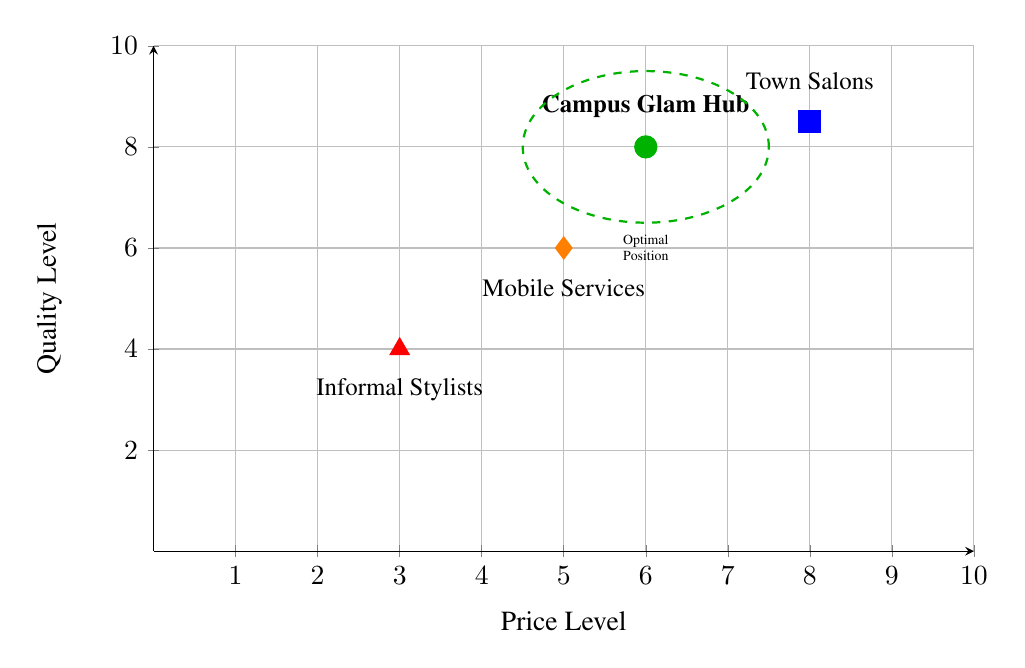
\begin{tikzpicture}
    \begin{axis}[
        xlabel={Price Level},
        ylabel={Quality Level},
        xmin=0, xmax=10,
        ymin=0, ymax=10,
        grid=major,
        width=12cm,
        height=8cm,
        legend pos=north west,
        axis lines=middle,
        xlabel style={at={(axis description cs:0.5,-0.1)},anchor=north},
        ylabel style={at={(axis description cs:-0.1,0.5)},rotate=90,anchor=south}
    ]
    
    % Campus Glam Hub
    \addplot[only marks, mark=*, mark size=4pt, color=green!70!black] 
        coordinates {(6,8)};
    \node at (axis cs:6,8.8) [font=\small\bfseries] {Campus Glam Hub};
    
    % Town Salons
    \addplot[only marks, mark=square*, mark size=4pt, color=blue] 
        coordinates {(8,8.5)};
    \node at (axis cs:8,9.3) [font=\small] {Town Salons};
    
    % Informal Stylists
    \addplot[only marks, mark=triangle*, mark size=4pt, color=red] 
        coordinates {(3,4)};
    \node at (axis cs:3,3.2) [font=\small] {Informal Stylists};
    
    % Mobile Services
    \addplot[only marks, mark=diamond*, mark size=4pt, color=orange] 
        coordinates {(5,6)};
    \node at (axis cs:5,5.2) [font=\small] {Mobile Services};
    
    % Sweet spot circle
    \draw[dashed, thick, color=green!70!black] (axis cs:6,8) circle [radius=1.5];
    \node at (axis cs:6,6) [font=\tiny, text width=2cm, align=center] {Optimal\\Position};
    
    \end{axis}
\end{tikzpicture}

\vspace{0.5em}
Campus Glam Hub occupies the optimal position: high quality at moderate prices, with unmatched convenience.
\end{center}

\vspace{1em}

% Competitive Comparison Table
\begin{center}
\textbf{Detailed Competitor Comparison}
\vspace{0.5em}

\begin{tabular}{|>{\raggedright\arraybackslash}p{2.5cm}|p{2.2cm}|p{2.2cm}|p{2.2cm}|p{2.2cm}|}
\hline
\rowcolor{primarycolor!20}
\textbf{Factor} & \textbf{Campus Glam Hub} & \textbf{Town Salons} & \textbf{Informal Stylists} & \textbf{Mobile Services} \\
\hline
Location & On campus & 5-10 km away & On campus & Variable \\
\hline
Price Range & UGX 10k-50k & UGX 15k-80k & UGX 5k-15k & UGX 10k-30k \\
\hline
Quality & High & High & Low-Medium & Medium \\
\hline
Convenience & Excellent & Poor & Good & Medium \\
\hline
Hygiene & Excellent & Good & Poor & Medium \\
\hline
Equipment & Professional & Professional & Basic & Limited \\
\hline
Service Range & Comprehensive & Comprehensive & Limited & Variable \\
\hline
Reliability & High & High & Low & Medium \\
\hline
\end{tabular}
\end{center}

\subsection{Trends and Market Forecasts}

\textbf{Current Trends:}
\begin{itemize}[leftmargin=2em]
    \item Natural hair care movement gaining popularity among students
    \item Increased demand for event makeup (graduations, parties, photoshoots)
    \item Growing interest in skincare routines and treatments
    \item Male grooming services becoming more accepted
    \item Social media driving demand for trendy hairstyles and makeup looks
\end{itemize}

\textbf{Market Forecast:}
\begin{itemize}[leftmargin=2em]
    \item Expected to capture 30\% of the campus market within the first year
    \item Projected customer base of 150-200 regular clients by month 6
    \item Anticipated 15-20\% growth in customer base annually
    \item Expansion potential to other university campuses in the region
\end{itemize}

%---------------- Marketing Plan ----------------%
\newpage
\section{Marketing Plan}

\subsection{Definition of the Overall Market}

The overall market for Campus Glam Hub consists of the beauty and personal care services market within the university setting. This includes all students, staff, and faculty at Mbarara University of Science and Technology who require hair, makeup, skincare, and grooming services. The market extends to the surrounding Kihumuro community, including residents and visitors to the campus area.

\subsection{Market Size and Growth}

\textbf{Primary Market:}
\begin{itemize}[leftmargin=2em]
    \item Total student population: Approximately 5,000 students
    \item Staff and faculty: Approximately 500 individuals
    \item Total primary market: 5,500 potential customers
\end{itemize}

\textbf{Secondary Market:}
\begin{itemize}[leftmargin=2em]
    \item Kihumuro community residents: Estimated 2,000 individuals
    \item Campus visitors and event attendees
\end{itemize}

\textbf{Growth Potential:}
\begin{itemize}[leftmargin=2em]
    \item University enrollment growing at 5\% annually
    \item Increasing awareness of personal grooming
    \item Expanding service offerings to capture larger market share
\end{itemize}

\vspace{1em}

% Market Size Pie Chart
\begin{center}
\textbf{Target Market Composition}
\vspace{0.5em}

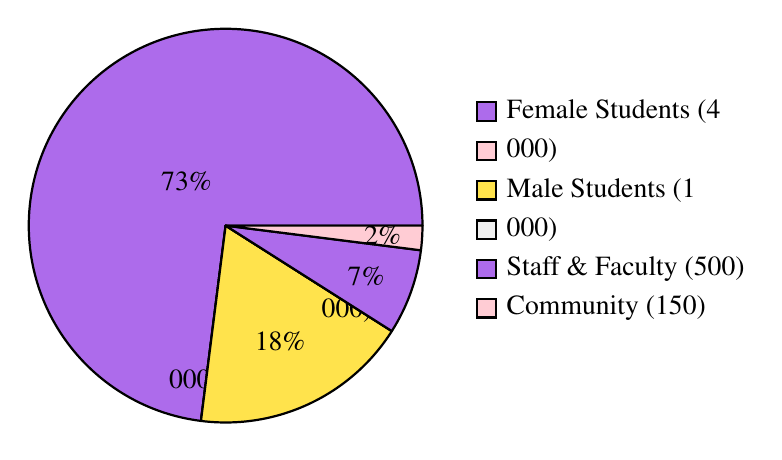
\begin{tikzpicture}
    \pie[
        text=legend,
        radius=2.5,
        color={primarycolor!70, secondarycolor!70, accentcolor!70, lightgray}
    ]{
        73/Female Students (4,000),
        18/Male Students (1,000),
        7/Staff \& Faculty (500),
        2/Community (150)
    }
\end{tikzpicture}
\end{center}

\vspace{1em}

% Market Growth Projection Chart
\begin{center}
\textbf{Market Growth Projection (5 Years)}
\vspace{0.5em}

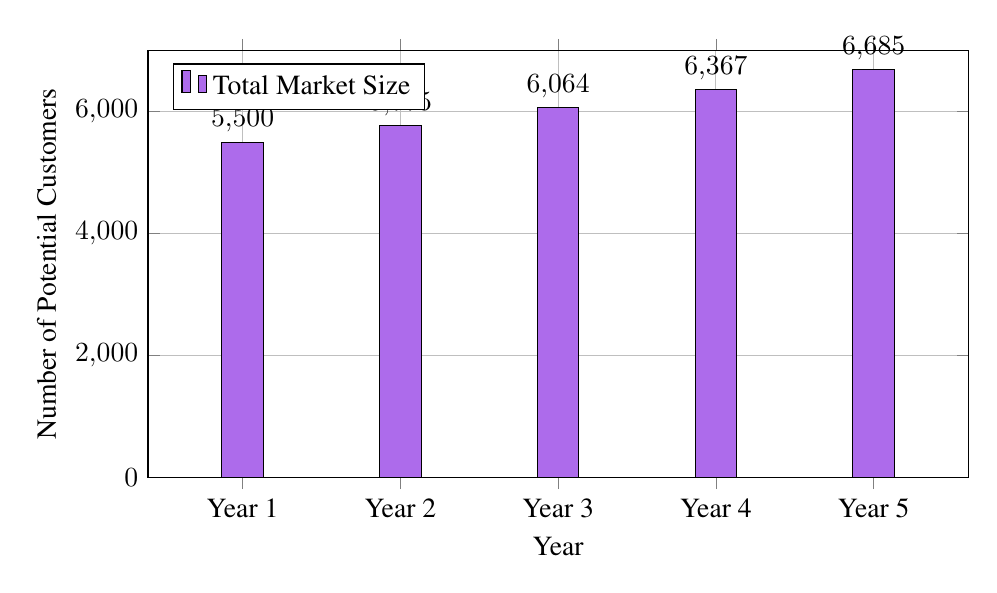
\begin{tikzpicture}
    \begin{axis}[
        ybar,
        bar width=15pt,
        xlabel={Year},
        ylabel={Number of Potential Customers},
        ymin=0,
        ymax=7000,
        xtick=data,
        symbolic x coords={Year 1, Year 2, Year 3, Year 4, Year 5},
        nodes near coords,
        nodes near coords align={vertical},
        width=12cm,
        height=7cm,
        legend pos=north west,
        grid=major,
        ymajorgrids=true,
        enlarge x limits=0.15
    ]
    
    \addplot[fill=primarycolor!70] coordinates {
        (Year 1, 5500)
        (Year 2, 5775)
        (Year 3, 6064)
        (Year 4, 6367)
        (Year 5, 6685)
    };
    
    \legend{Total Market Size}
    
    \end{axis}
\end{tikzpicture}

\vspace{0.5em}
Market growing at 5\% annually due to increasing university enrollment and community awareness.
\end{center}

\subsection{Market Trends}

\begin{itemize}[leftmargin=2em]
    \item Shift towards convenience-based services
    \item Preference for affordable, student-friendly pricing
    \item Demand for quick service during breaks between classes
    \item Interest in trendy, social media-inspired styles
    \item Growing male grooming market
    \item Increased spending on special occasion services (graduations, parties)
\end{itemize}

\subsection{Market Segments}

\textbf{Segment 1: Female Students (Primary - 60\% of market)}
\begin{itemize}[leftmargin=2em]
    \item Age: 18-25 years
    \item Needs: Regular hair maintenance, event makeup, nail services
    \item Frequency: 2-4 visits per month
    \item Price sensitivity: High
\end{itemize}

\textbf{Segment 2: Male Students (Growing - 20\% of market)}
\begin{itemize}[leftmargin=2em]
    \item Age: 18-25 years
    \item Needs: Haircuts, grooming services
    \item Frequency: 1-2 visits per month
    \item Price sensitivity: High
\end{itemize}

\textbf{Segment 3: Staff and Faculty (15\% of market)}
\begin{itemize}[leftmargin=2em]
    \item Age: 25-55 years
    \item Needs: Professional styling, skincare, full grooming services
    \item Frequency: 2-3 visits per month
    \item Price sensitivity: Medium
\end{itemize}

\textbf{Segment 4: Community Members (5\% of market)}
\begin{itemize}[leftmargin=2em]
    \item Age: Various
    \item Needs: All services, special occasion styling
    \item Frequency: Occasional
    \item Price sensitivity: Medium to low
\end{itemize}

\vspace{1em}

% Market Segmentation Visual
\begin{center}
\textbf{Market Segmentation Strategy}
\vspace{0.5em}

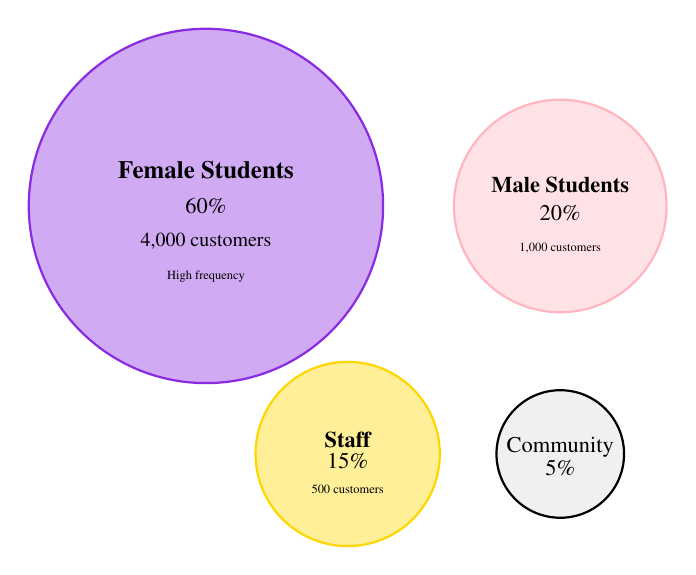
\begin{tikzpicture}[scale=0.9, transform shape]
    % Female Students - Largest circle
    \draw[fill=primarycolor!40, draw=primarycolor, thick] (0,0) circle (2.5cm);
    \node at (0,0.5) [font=\bfseries] {Female Students};
    \node at (0,0) [font=\small] {60\%};
    \node at (0,-0.5) [font=\footnotesize] {4,000 customers};
    \node at (0,-1) [font=\tiny] {High frequency};
    
    % Male Students
    \draw[fill=secondarycolor!40, draw=secondarycolor, thick] (5,0) circle (1.5cm);
    \node at (5,0.3) [font=\bfseries\small] {Male Students};
    \node at (5,-0.1) [font=\small] {20\%};
    \node at (5,-0.6) [font=\tiny] {1,000 customers};
    
    % Staff & Faculty
    \draw[fill=accentcolor!40, draw=accentcolor, thick] (2,-3.5) circle (1.3cm);
    \node at (2,-3.3) [font=\bfseries\small] {Staff};
    \node at (2,-3.6) [font=\small] {15\%};
    \node at (2,-4) [font=\tiny] {500 customers};
    
    % Community
    \draw[fill=lightgray, draw=black, thick] (5,-3.5) circle (0.9cm);
    \node at (5,-3.4) [font=\small] {Community};
    \node at (5,-3.7) [font=\small] {5\%};
    
\end{tikzpicture}
\end{center}

\vspace{1em}

\begin{tcolorbox}[mybox, title=\textbf{Market Segmentation Insights}]
\textbf{Why Female Students are Primary Target:}
\begin{itemize}[leftmargin=1em, itemsep=0pt]
    \item Highest frequency of service usage (2-4 times/month)
    \item Wide range of service needs (hair, makeup, nails, skincare)
    \item Strong word-of-mouth influence within campus
    \item Active on social media, providing free marketing
    \item Loyal customers when satisfied with service
\end{itemize}

\textbf{Growing Male Market Opportunity:}
\begin{itemize}[leftmargin=1em, itemsep=0pt]
    \item Increasing acceptance of male grooming
    \item Regular haircut needs (every 2-3 weeks)
    \item Potential for specialized men's grooming services
    \item Less price-sensitive for quality services
\end{itemize}
\end{tcolorbox}

\subsection{Customer Characteristics and Needs}

\textbf{Detailed Customer Characteristics:}

\textbf{Demographics:}
\begin{itemize}[leftmargin=2em]
    \item Age Range: Primarily 18-25 years (students), 25-55 years (staff)
    \item Gender Distribution: 60\% female, 40\% male
    \item Income Level: Students (UGX 50,000-200,000 monthly allowance), Staff (UGX 500,000-2,000,000 monthly salary)
    \item Education Level: Undergraduate and postgraduate students, university staff with tertiary education
    \item Location: Primarily residing on or near Kihumuro Campus
\end{itemize}

\textbf{Psychographics:}
\begin{itemize}[leftmargin=2em]
    \item Lifestyle: Active, social, academically focused
    \item Values: Convenience, affordability, quality, authenticity
    \item Interests: Fashion, social media, campus events, personal development
    \item Personality: Trend-conscious, socially aware, budget-conscious but willing to invest in appearance
    \item Attitudes: Positive towards self-care, value time efficiency, appreciate personalized service
\end{itemize}

\textbf{Behavioral Characteristics:}
\begin{itemize}[leftmargin=2em]
    \item Purchase Frequency: Students 2-4 times monthly, Staff 2-3 times monthly
    \item Service Preferences: Hair services most popular, followed by makeup for events
    \item Decision Factors: Price (40\%), convenience (35\%), quality (20\%), recommendations (5\%)
    \item Brand Loyalty: Moderate to high when satisfied with service
    \item Information Sources: Social media (60\%), word-of-mouth (30\%), campus advertising (10\%)
    \item Booking Preferences: WhatsApp booking (50\%), walk-in (40\%), phone call (10\%)
\end{itemize}

\textbf{Technology Usage:}
\begin{itemize}[leftmargin=2em]
    \item Smartphone Ownership: 95\% of target market
    \item Social Media Platforms: Instagram (80\%), Facebook (70\%), TikTok (60\%), WhatsApp (95\%)
    \item Mobile Money Usage: 85\% regularly use mobile money for transactions
    \item Online Research: 70\% research services online before visiting
\end{itemize}

\vspace{1em}

\textbf{Detailed Customer Needs Analysis:}

\textbf{Functional Needs:}
\begin{itemize}[leftmargin=2em]
    \item Affordable Pricing: Services priced 15-20\% below town rates to fit student budgets
    \item Convenient Location: On-campus location eliminates 5-10km travel to town
    \item Time Efficiency: Services completed within estimated timeframes, minimal waiting
    \item Flexible Scheduling: Operating hours 8 AM-8 PM weekdays accommodate class schedules
    \item Quality Results: Professional-grade services using quality products and trained staff
    \item Service Variety: Comprehensive range from basic maintenance to special occasion styling
    \item Hygiene Standards: Clean, sanitized environment with proper sterilization protocols
    \item Quick Options: Express services available for customers with limited time
\end{itemize}

\textbf{Emotional Needs:}
\begin{itemize}[leftmargin=2em]
    \item Confidence Boost: Services that enhance appearance and self-esteem
    \item Relaxation: Comfortable, stress-free environment away from academic pressures
    \item Social Acceptance: Trendy styles that align with campus fashion standards
    \item Personal Expression: Ability to customize services to individual style preferences
    \item Trust: Reliable service providers who understand their needs
    \item Belonging: Welcoming atmosphere where they feel valued as customers
\end{itemize}

\textbf{Social Needs:}
\begin{itemize}[leftmargin=2em]
    \item Peer Approval: Styles that receive positive feedback from friends and classmates
    \item Event Readiness: Professional styling for campus events, parties, and graduations
    \item Social Media Presence: Looks that photograph well for Instagram, TikTok, and Facebook
    \item Community Connection: Salon as social space to meet friends and socialize
\end{itemize}

\textbf{Practical Needs:}
\begin{itemize}[leftmargin=2em]
    \item Payment Flexibility: Accept cash and mobile money (MTN, Airtel)
    \item Easy Booking: Simple appointment system via WhatsApp or walk-in
    \item Transparent Pricing: Clear price lists with no hidden charges
    \item Product Availability: Retail products for home maintenance between visits
    \item Aftercare Advice: Guidance on maintaining styles and treatments
    \item Loyalty Rewards: Programs that recognize and reward regular customers
\end{itemize}

\vspace{1em}

\textbf{Customer Personas:}

\textbf{Persona 1: "Fashionable Fiona" - Female Student}
\begin{itemize}[leftmargin=2em]
    \item Age: 21, 3rd year Business Administration student
    \item Monthly Budget: UGX 150,000 allowance
    \item Beauty Spending: UGX 40,000-60,000 monthly
    \item Frequency: Visits 3-4 times per month
    \item Preferred Services: Hair braiding, makeup for events, nail services
    \item Motivations: Wants to look good for social media, campus events, and daily classes
    \item Pain Points: Town salons too expensive with transport, informal stylists unreliable
    \item Decision Factors: Price (high importance), trendiness (high), convenience (high)
    \item Quote: "I need to look good without spending my entire allowance on transport and salon fees"
\end{itemize}

\textbf{Persona 2: "Busy Brian" - Male Student}
\begin{itemize}[leftmargin=2em]
    \item Age: 23, 4th year Computer Science student
    \item Monthly Budget: UGX 100,000 allowance
    \item Beauty Spending: UGX 15,000-25,000 monthly
    \item Frequency: Visits 2 times per month
    \item Preferred Services: Haircuts, beard trimming, occasional facial
    \item Motivations: Maintain professional appearance, save time
    \item Pain Points: No time to travel to town, wants quick service between classes
    \item Decision Factors: Convenience (very high), speed (high), quality (medium)
    \item Quote: "I just need a quick, quality haircut without wasting half my day traveling"
\end{itemize}

\textbf{Persona 3: "Professional Patricia" - University Lecturer}
\begin{itemize}[leftmargin=2em]
    \item Age: 35, Lecturer in Faculty of Science
    \item Monthly Income: UGX 1,200,000
    \item Beauty Spending: UGX 80,000-120,000 monthly
    \item Frequency: Visits 2-3 times per month
    \item Preferred Services: Professional styling, skincare treatments, full grooming
    \item Motivations: Maintain professional appearance, convenience during work hours
    \item Pain Points: Limited time to travel to town during work hours
    \item Decision Factors: Quality (very high), convenience (high), professionalism (high)
    \item Quote: "I need professional services without leaving campus during my busy schedule"
\end{itemize}

\textbf{Persona 4: "Event-Ready Emma" - Female Student}
\begin{itemize}[leftmargin=2em]
    \item Age: 20, 2nd year Education student
    \item Monthly Budget: UGX 80,000 allowance
    \item Beauty Spending: UGX 20,000-40,000 monthly (spikes for events)
    \item Frequency: Visits 1-2 times monthly, more during event season
    \item Preferred Services: Event makeup, special occasion hairstyles
    \item Motivations: Look stunning for graduations, parties, photoshoots
    \item Pain Points: Town salons booked up during event season, expensive packages
    \item Decision Factors: Quality for events (very high), affordability (high), availability (high)
    \item Quote: "I need to look amazing for my friend's graduation without breaking the bank"
\end{itemize}

\vspace{1em}

\begin{tcolorbox}[mybox, title=\textbf{Customer Insights Summary}]
\textbf{Key Takeaways from Customer Analysis:}
\begin{itemize}[leftmargin=1em, itemsep=0pt]
    \item \textbf{Convenience is King:} 85\% of customers cite convenience as top factor
    \item \textbf{Price Sensitivity:} Students willing to pay for quality but need affordable options
    \item \textbf{Time-Starved:} Average customer has less than 2 hours for beauty services
    \item \textbf{Social Media Influence:} 70\% discover services through Instagram/TikTok
    \item \textbf{Word-of-Mouth Power:} 90\% trust recommendations from friends
    \item \textbf{Event-Driven Demand:} 40\% spike in demand during graduation season
    \item \textbf{Mobile-First:} 95\% prefer WhatsApp booking over phone calls
    \item \textbf{Loyalty Potential:} 75\% become regular customers when satisfied
\end{itemize}

\textbf{Strategic Implications:}
\begin{itemize}[leftmargin=1em, itemsep=0pt]
    \item Focus marketing on convenience and cost savings
    \item Invest heavily in social media presence
    \item Create express service options for time-constrained customers
    \item Develop event packages for graduation season
    \item Implement WhatsApp-based booking system
    \item Build loyalty program to encourage repeat visits
    \item Train staff in personalized customer service
\end{itemize}
\end{tcolorbox}

\subsection{Competitors Products and Market Share}

\textbf{Comprehensive Competitor Analysis:}

\textbf{Competitor 1: Mbarara Town Beauty Salons}

\textbf{Overview:}
\begin{itemize}[leftmargin=2em]
    \item Number of Competitors: 15-20 established salons in Mbarara town
    \item Distance from Campus: 5-10 kilometers
    \item Market Share: 50\% of campus market (approximately 2,750 customers)
    \item Years in Operation: Most established 5-15 years
\end{itemize}

\textbf{Service Offerings:}
\begin{itemize}[leftmargin=2em]
    \item Hair Services: Haircuts (UGX 15,000-25,000), Braiding (UGX 20,000-50,000), Weaving (UGX 30,000-80,000), Coloring (UGX 40,000-100,000)
    \item Makeup Services: Event makeup (UGX 30,000-60,000), Bridal makeup (UGX 80,000-150,000)
    \item Skincare: Facials (UGX 25,000-50,000), Treatments (UGX 30,000-70,000)
    \item Nail Services: Manicure (UGX 15,000-25,000), Pedicure (UGX 20,000-35,000), Gel nails (UGX 30,000-50,000)
    \item Additional: Hair treatments, spa services, waxing
\end{itemize}

\textbf{Pricing Strategy:}
\begin{itemize}[leftmargin=2em]
    \item Premium Pricing: 20-30\% higher than Campus Glam Hub planned prices
    \item Target Market: General population, working professionals, higher-income customers
    \item Payment Methods: Cash, mobile money, some accept cards
    \item Discounts: Occasional promotions, package deals
\end{itemize}

\textbf{Strengths:}
\begin{itemize}[leftmargin=2em]
    \item Established Brand Recognition: Years of operation build trust and reputation
    \item Experienced Staff: Highly trained beauticians with 5-15 years experience
    \item Professional Equipment: High-end salon equipment and quality products
    \item Wide Service Range: Comprehensive services including specialized treatments
    \item Strong Supplier Relationships: Established connections for product sourcing
    \item Loyal Customer Base: Regular customers from town and surrounding areas
    \item Professional Facilities: Well-designed, comfortable salon environments
    \item Marketing Budget: Ability to invest in advertising and promotions
\end{itemize}

\textbf{Weaknesses:}
\begin{itemize}[leftmargin=2em]
    \item Distance from Campus: 5-10km requires transportation
    \item Transportation Costs: Students spend UGX 4,000-10,000 per round trip
    \item Time Consumption: 2-3 hours total including travel time
    \item Operating Hours: Typically 9 AM-6 PM, conflicts with class schedules
    \item Higher Pricing: 20-30\% more expensive than campus-based alternative
    \item Not Student-Focused: Services and atmosphere not tailored to student needs
    \item Limited Student Discounts: Few offer meaningful student pricing
    \item Booking Challenges: Often fully booked during peak times (weekends, events)
\end{itemize}

\textbf{Market Position:}
\begin{itemize}[leftmargin=2em]
    \item Currently serve 50\% of students who use professional beauty services
    \item Strong position with staff and faculty who have higher budgets
    \item Dominant during special occasions when quality is priority over convenience
    \item Vulnerable to campus-based competition due to convenience factor
\end{itemize}

\vspace{1em}

\textbf{Competitor 2: Informal Campus Stylists}

\textbf{Overview:}
\begin{itemize}[leftmargin=2em]
    \item Number of Competitors: 30-50 individuals operating informally
    \item Location: Hostels, homes near campus, informal settings
    \item Market Share: 30\% of campus market (approximately 1,650 customers)
    \item Business Model: Individual operators, no formal business structure
\end{itemize}

\textbf{Service Offerings:}
\begin{itemize}[leftmargin=2em]
    \item Hair Services: Basic braiding (UGX 5,000-15,000), Simple hairstyles (UGX 3,000-10,000), Hair washing (UGX 2,000-5,000)
    \item Limited Makeup: Basic makeup for events (UGX 10,000-20,000)
    \item Nail Services: Basic manicure (UGX 5,000-10,000)
    \item No Advanced Services: Cannot provide complex treatments, coloring, or specialized services
\end{itemize}

\textbf{Pricing Strategy:}
\begin{itemize}[leftmargin=2em]
    \item Ultra-Low Pricing: 50-70\% below professional salon rates
    \item Target Market: Price-sensitive students, those seeking basic services
    \item Payment Methods: Cash only, sometimes barter or deferred payment
    \item Negotiable Prices: Often willing to negotiate based on customer relationship
\end{itemize}

\textbf{Strengths:}
\begin{itemize}[leftmargin=2em]
    \item Very Low Prices: Most affordable option available
    \item Convenient Location: On or very near campus
    \item Flexible Hours: Often available evenings and weekends
    \item Personal Relationships: Know customers personally, friendly atmosphere
    \item No Overhead Costs: Operating from homes keeps costs minimal
    \item Flexible Payment: May accept deferred payment or barter
    \item Quick Booking: Often available on short notice
\end{itemize}

\textbf{Weaknesses:}
\begin{itemize}[leftmargin=2em]
    \item Inconsistent Quality: Results vary widely, no quality standards
    \item Limited Services: Cannot provide complex or specialized treatments
    \item Basic Equipment: Lack professional tools and equipment
    \item Hygiene Concerns: Often inadequate sanitation and sterilization
    \item No Professional Training: Most lack formal beauty training or certification
    \item Unreliable Availability: May not be available when needed
    \item No Recourse: No formal complaint process or service guarantees
    \item Limited Products: Use basic, often low-quality products
    \item Unprofessional Environment: Informal settings lack salon atmosphere
    \item No Insurance: No liability coverage for accidents or poor results
\end{itemize}

\textbf{Market Position:}
\begin{itemize}[leftmargin=2em]
    \item Serve 30\% of market, primarily price-sensitive students
    \item Strong position for basic, routine services
    \item Vulnerable to professional competition offering reasonable prices
    \item May lose customers as students gain more disposable income
\end{itemize}

\vspace{1em}

\textbf{Competitor 3: Mobile Beauty Service Providers}

\textbf{Overview:}
\begin{itemize}[leftmargin=2em]
    \item Number of Competitors: 10-15 mobile service providers
    \item Service Area: Travel to customer locations (hostels, homes)
    \item Market Share: 10\% of campus market (approximately 550 customers)
    \item Business Model: Individual practitioners or small teams
\end{itemize}

\textbf{Service Offerings:}
\begin{itemize}[leftmargin=2em]
    \item Hair Services: Braiding (UGX 15,000-35,000), Simple styling (UGX 10,000-25,000)
    \item Makeup Services: Event makeup (UGX 20,000-40,000), Bridal makeup (UGX 60,000-120,000)
    \item Limited Treatments: Only services that can be performed with portable equipment
    \item Specialized Services: Some focus on specific services (makeup only, braiding only)
\end{itemize}

\textbf{Pricing Strategy:}
\begin{itemize}[leftmargin=2em]
    \item Premium for Convenience: 20-40\% higher than salon prices to cover travel
    \item Target Market: Customers willing to pay for convenience, event services
    \item Payment Methods: Cash, mobile money
    \item Booking Fees: Some charge booking or travel fees
\end{itemize}

\textbf{Strengths:}
\begin{itemize}[leftmargin=2em]
    \item Ultimate Convenience: Service at customer's location
    \item Flexible Scheduling: Can accommodate unusual hours
    \item Personal Service: One-on-one attention
    \item Privacy: Service in customer's private space
    \item No Travel Required: Customer saves time and transport costs
    \item Event Specialization: Many specialize in event makeup and styling
\end{itemize}

\textbf{Weaknesses:}
\begin{itemize}[leftmargin=2em]
    \item Higher Prices: Premium pricing for convenience
    \item Limited Equipment: Cannot bring full salon equipment
    \item Service Limitations: Cannot provide services requiring fixed equipment
    \item Unreliable Scheduling: May cancel or arrive late
    \item Inconsistent Availability: Limited capacity, often booked up
    \item Quality Variability: Results depend on working conditions at location
    \item No Professional Environment: Lack of salon atmosphere and amenities
    \item Verification Challenges: Difficult to verify quality before booking
    \item Limited Product Range: Can only carry limited products
\end{itemize}

\textbf{Market Position:}
\begin{itemize}[leftmargin=2em]
    \item Serve 10\% of market, primarily for special occasions
    \item Strong position for event services (graduations, weddings)
    \item Vulnerable to professional salon with convenient location
    \item May retain customers who specifically value at-home service
\end{itemize}

\vspace{1em}

\textbf{Competitor 4: DIY and Home Treatments}

\textbf{Overview:}
\begin{itemize}[leftmargin=2em]
    \item Market Share: 10\% of potential market (approximately 550 individuals)
    \item Approach: Self-service or help from friends
    \item Cost: Only product costs, no service fees
\end{itemize}

\textbf{Strengths:}
\begin{itemize}[leftmargin=2em]
    \item Lowest Cost: Only pay for products
    \item Complete Flexibility: Do services anytime
    \item Learning Opportunity: Develop personal skills
    \item Privacy: Complete privacy at home
\end{itemize}

\textbf{Weaknesses:}
\begin{itemize}[leftmargin=2em]
    \item Limited to Simple Services: Cannot achieve complex styles
    \item Time-Consuming: Takes much longer than professional service
    \item Inconsistent Results: Often inferior to professional results
    \item Risk of Damage: Potential for hair or skin damage
    \item No Professional Products: Limited access to quality products
    \item No Expertise: Lack professional knowledge and techniques
\end{itemize}

\vspace{1em}

\textbf{Competitive Comparison Matrix:}

\begin{center}
\begin{tabular}{|l|c|c|c|c|c|}
\hline
\textbf{Factor} & \textbf{Campus} & \textbf{Town} & \textbf{Informal} & \textbf{Mobile} & \textbf{DIY} \\
 & \textbf{Glam Hub} & \textbf{Salons} & \textbf{Stylists} & \textbf{Services} & \\
\hline
Price & Medium & High & Very Low & High & Very Low \\
\hline
Quality & High & High & Low & Medium & Low \\
\hline
Convenience & Very High & Low & High & Very High & High \\
\hline
Service Range & High & Very High & Low & Medium & Very Low \\
\hline
Professionalism & High & Very High & Low & Medium & N/A \\
\hline
Reliability & High & High & Low & Medium & High \\
\hline
Hygiene & High & High & Low & Medium & Medium \\
\hline
\end{tabular}
\end{center}

\vspace{1em}

\textbf{Campus Glam Hub Competitive Advantages:}

\textbf{Against Town Salons:}
\begin{itemize}[leftmargin=2em]
    \item Save UGX 4,000-10,000 transportation costs per visit
    \item Save 1-2 hours travel time per visit
    \item 15-20\% lower base pricing
    \item Total savings of 30-40\% per visit
    \item Extended hours better suited to student schedules
    \item No booking conflicts with class times
    \item Student-focused atmosphere and service approach
\end{itemize}

\textbf{Against Informal Stylists:}
\begin{itemize}[leftmargin=2em]
    \item Professional quality and consistency
    \item Comprehensive service range including advanced treatments
    \item Professional equipment and quality products
    \item Hygienic, safe, regulated environment
    \item Trained, certified staff with proven expertise
    \item Reliable availability and scheduling
    \item Service guarantees and complaint resolution
    \item Professional atmosphere and amenities
    \item Only 20-30\% higher pricing for significantly better quality
\end{itemize}

\textbf{Against Mobile Services:}
\begin{itemize}[leftmargin=2em]
    \item Lower pricing (30-40\% less)
    \item Full range of equipment and services
    \item Consistent availability
    \item Professional facility with all amenities
    \item No scheduling uncertainty
    \item Established location for easy access
    \item Better quality control
\end{itemize}

\textbf{Against DIY:}
\begin{itemize}[leftmargin=2em]
    \item Professional results worth the investment
    \item Significant time savings
    \item Access to professional products and equipment
    \item Expert advice and consultation
    \item Complex styles and treatments possible
    \item Reduced risk of poor results or damage
    \item Relaxing experience vs. stressful DIY attempts
\end{itemize}

\vspace{1em}

\textbf{Campus Glam Hub Target Market Share:}
\begin{itemize}[leftmargin=2em]
    \item Year 1: 30\% of campus market (1,650 customers) - capturing from all competitor segments
    \item Year 2: 45\% of campus market (2,600 customers) - primarily from town salons and informal stylists
    \item Year 3: 55\% of campus market (3,300 customers) - becoming dominant campus provider
    \item Year 4: 60\% of campus market (3,800 customers) - market leader position
    \item Year 5: 65\% of campus market (4,350 customers) - strong market dominance
\end{itemize}

\textbf{Market Share Capture Strategy:}
\begin{itemize}[leftmargin=2em]
    \item From Town Salons (50\% share): Capture 40\% of their campus customers through convenience and cost advantages
    \item From Informal Stylists (30\% share): Capture 50\% of their customers through quality and professionalism at reasonable prices
    \item From Mobile Services (10\% share): Capture 60\% of their customers through better pricing and consistent availability
    \item From DIY (10\% share): Capture 30\% by offering affordable professional alternative
    \item New Market Creation: Attract 500+ customers who currently don't use beauty services due to barriers
\end{itemize}

\subsection{Future Competitors}

\textbf{Comprehensive Future Competition Analysis:}

\textbf{Potential Future Competitor 1: Copycat Campus-Based Salons}

\textbf{Threat Level:} High (Likelihood: Medium, Impact: High)

\textbf{Description:}
\begin{itemize}[leftmargin=2em]
    \item Other entrepreneurs observing Campus Glam Hub's success may attempt to establish similar campus-based salons
    \item Could emerge within 12-24 months after our launch
    \item May target same customer base with similar value proposition
    \item Could appear on Mbarara University campus or other nearby campuses
\end{itemize}

\textbf{Potential Advantages They May Have:}
\begin{itemize}[leftmargin=2em]
    \item Learn from our mistakes and successes
    \item May have larger initial capital investment
    \item Could offer lower prices to gain market share
    \item Might bring innovative services or technology
\end{itemize}

\textbf{Our Defensive Strategies:}
\begin{itemize}[leftmargin=2em]
    \item First-Mover Advantage: Establish strong brand recognition before competitors enter
    \item Customer Loyalty Programs: Lock in customers with rewards and incentives
    \item Exclusive Partnerships: Secure exclusive agreements with student organizations
    \item Prime Location: Secure best available campus location with long-term lease
    \item Quality Reputation: Build unassailable reputation for quality and service
    \item Continuous Innovation: Regularly introduce new services and improvements
    \item Staff Retention: Retain skilled staff through competitive compensation
    \item Price Competitiveness: Maintain pricing that makes market entry unattractive
\end{itemize}

\vspace{1em}

\textbf{Potential Future Competitor 2: Mobile Beauty Service Apps}

\textbf{Threat Level:} Medium (Likelihood: Medium, Impact: Medium)

\textbf{Description:}
\begin{itemize}[leftmargin=2em]
    \item Technology-enabled platforms connecting beauty professionals with customers
    \item Similar to Uber model but for beauty services
    \item May expand from Kampala to Mbarara area
    \item Could offer convenience of at-home service with professional quality
\end{itemize}

\textbf{Potential Advantages They May Have:}
\begin{itemize}[leftmargin=2em]
    \item Technology platform for easy booking and payment
    \item Network of multiple service providers
    \item Convenience of at-home service
    \item Marketing budget from venture capital funding
    \item Data-driven pricing and service optimization
\end{itemize}

\textbf{Our Defensive Strategies:}
\begin{itemize}[leftmargin=2em]
    \item Professional Facility Advantage: Full equipment range not available for mobile services
    \item Competitive Pricing: Price competitively against mobile service premiums
    \item Technology Adoption: Implement our own booking app or WhatsApp Business
    \item Service Range: Offer services that cannot be provided mobile (treatments requiring fixed equipment)
    \item Reliability: Consistent availability vs. variable mobile provider availability
    \item Community Connection: Strong campus community ties vs. impersonal app
    \item Immediate Service: Walk-in availability vs. advance booking requirements
\end{itemize}

\vspace{1em}

\textbf{Potential Future Competitor 3: Professionalized Informal Stylists}

\textbf{Threat Level:} Medium (Likelihood: High, Impact: Low)

\textbf{Description:}
\begin{itemize}[leftmargin=2em]
    \item Current informal campus stylists may professionalize their operations
    \item Could obtain training, equipment, and formal business registration
    \item May establish small professional setups near campus
    \item Retain existing customer relationships while improving quality
\end{itemize}

\textbf{Potential Advantages They May Have:}
\begin{itemize}[leftmargin=2em]
    \item Established customer relationships
    \item Lower overhead from home-based operations
    \item Flexible pricing and payment terms
    \item Personal connection with customers
    \item May still offer lower prices than formal salons
\end{itemize}

\textbf{Our Defensive Strategies:}
\begin{itemize}[leftmargin=2em]
    \item Professional Environment: Full salon experience vs. home-based setup
    \item Comprehensive Services: Wide range of services vs. limited offerings
    \item Brand Trust: Professional brand vs. individual operator
    \item Consistent Quality: Quality standards and supervision
    \item Scalability: Ability to serve multiple customers simultaneously
    \item Professional Products: Access to quality professional products
    \item Recruitment: Potentially recruit talented informal stylists to join our team
\end{itemize}

\vspace{1em}

\textbf{Potential Future Competitor 4: New Town Salons Near Campus}

\textbf{Threat Level:} Medium (Likelihood: Low, Impact: Medium)

\textbf{Description:}
\begin{itemize}[leftmargin=2em]
    \item Established town salons may open branches closer to campus
    \item New salons may open in areas between campus and town
    \item Could reduce travel distance and time for students
    \item May target campus market specifically
\end{itemize}

\textbf{Potential Advantages They May Have:}
\begin{itemize}[leftmargin=2em]
    \item Established brand reputation
    \item Experience and expertise
    \item Financial resources for quality setup
    \item Supplier relationships
    \item Marketing capabilities
\end{itemize}

\textbf{Our Defensive Strategies:}
\begin{itemize}[leftmargin=2em]
    \item On-Campus Location: Still more convenient than near-campus locations
    \item Student-Focused: Specifically designed for student needs vs. general market
    \item Pricing Advantage: Lower pricing tailored to student budgets
    \item Campus Integration: Deep integration with campus community and events
    \item Brand Loyalty: Established relationships with student customers
    \item Operating Hours: Hours specifically designed for student schedules
\end{itemize}

\vspace{1em}

\textbf{Potential Future Competitor 5: Chain Salon Expansion}

\textbf{Threat Level:} Low (Likelihood: Very Low, Impact: High if occurs)

\textbf{Description:}
\begin{itemize}[leftmargin=2em]
    \item National or regional salon chains may expand to Mbarara
    \item Could bring significant capital, brand recognition, and expertise
    \item May target campus market as part of broader Mbarara expansion
    \item Unlikely in short-term but possible in 3-5 years
\end{itemize}

\textbf{Potential Advantages They May Have:}
\begin{itemize}[leftmargin=2em]
    \item Strong brand recognition
    \item Significant financial resources
    \item Economies of scale in purchasing
    \item Professional management systems
    \item Marketing expertise and budget
    \item Standardized quality systems
\end{itemize}

\textbf{Our Defensive Strategies:}
\begin{itemize}[leftmargin=2em]
    \item Local Knowledge: Deep understanding of campus market vs. generic approach
    \item Personal Service: Personalized attention vs. standardized service
    \item Flexibility: Quick adaptation to market needs vs. corporate bureaucracy
    \item Community Connection: Strong local relationships vs. corporate brand
    \item Niche Focus: Specialized campus focus vs. general market approach
    \item Potential Partnership: Possibility of franchise or partnership arrangement
    \item By then, Strong Position: 3-5 years to establish unassailable market position
\end{itemize}

\vspace{1em}

\textbf{Barriers to Entry We Create:}

\textbf{Strategic Barriers:}
\begin{itemize}[leftmargin=2em]
    \item First-Mover Advantage: Being first campus-based salon creates strong brand recognition
    \item Brand Loyalty: Loyalty programs and excellent service create switching costs
    \item Location Advantage: Prime campus location may not be available to competitors
    \item Established Relationships: Partnerships with student organizations and campus administration
    \item Market Knowledge: Deep understanding of campus market and customer preferences
    \item Reputation: Strong reputation for quality and service difficult to replicate
\end{itemize}

\textbf{Operational Barriers:}
\begin{itemize}[leftmargin=2em]
    \item Economies of Scale: Established supplier relationships and bulk purchasing
    \item Trained Staff: Skilled, experienced team familiar with campus market
    \item Systems and Processes: Refined operational systems and procedures
    \item Customer Database: Valuable customer data and preferences
    \item Efficient Operations: Optimized processes reduce costs and improve service
\end{itemize}

\textbf{Financial Barriers:}
\begin{itemize}[leftmargin=2em]
    \item Capital Requirements: Significant investment needed for quality setup
    \item Break-Even Timeline: 12-18 months to profitability deters some competitors
    \item Price Competition: Our competitive pricing makes market entry less attractive
    \item Customer Acquisition Costs: High costs to attract customers from established provider
\end{itemize}

\textbf{Regulatory Barriers:}
\begin{itemize}[leftmargin=2em]
    \item Campus Approvals: May be difficult to obtain permission for campus operations
    \item Business Licenses: Regulatory requirements and compliance costs
    \item Health and Safety: Standards and inspections create compliance burden
    \item Insurance Requirements: Liability insurance and other coverage requirements
\end{itemize}

\vspace{1em}

\textbf{Competitive Response Plan:}

\textbf{If New Competitor Enters Market:}
\begin{enumerate}[leftmargin=2em]
    \item \textbf{Assess Threat Level:} Analyze competitor's strengths, weaknesses, and strategy
    \item \textbf{Strengthen Customer Relationships:} Increase loyalty program benefits, personalized outreach
    \item \textbf{Service Innovation:} Introduce new services or improvements to differentiate
    \item \textbf{Pricing Strategy:} Evaluate pricing competitiveness, adjust if necessary
    \item \textbf{Marketing Intensification:} Increase marketing efforts to maintain visibility
    \item \textbf{Quality Enhancement:} Ensure service quality remains superior
    \item \textbf{Staff Retention:} Protect against staff poaching with competitive compensation
    \item \textbf{Customer Feedback:} Intensify feedback collection to identify and address concerns
\end{enumerate}

\textbf{Proactive Competition Prevention:}
\begin{itemize}[leftmargin=2em]
    \item Continuous Improvement: Regular service enhancements and innovations
    \item Customer Satisfaction: Maintain high satisfaction to reduce switching likelihood
    \item Market Monitoring: Track potential competitors and market changes
    \item Strategic Partnerships: Build exclusive relationships that create barriers
    \item Expansion Planning: Consider expansion to other campuses before competitors
    \item Brand Building: Invest in strong brand that creates emotional connection
    \item Community Engagement: Deep integration with campus community
\end{itemize}

\vspace{1em}

\begin{tcolorbox}[mybox, title=\textbf{Competitive Advantage Sustainability}]
\textbf{Our Sustainable Competitive Advantages:}
\begin{itemize}[leftmargin=1em, itemsep=0pt]
    \item \textbf{Location:} On-campus location provides unmatched convenience (hard to replicate)
    \item \textbf{First-Mover:} Brand recognition and customer loyalty from being first (time-based advantage)
    \item \textbf{Relationships:} Deep campus community connections (relationship-based advantage)
    \item \textbf{Knowledge:} Understanding of campus market nuances (knowledge-based advantage)
    \item \textbf{Reputation:} Quality and service reputation (reputation-based advantage)
    \item \textbf{Systems:} Refined operational systems (operational advantage)
\end{itemize}

\textbf{Competitive Moat Strategy:}
\begin{itemize}[leftmargin=1em, itemsep=0pt]
    \item Build strong brand loyalty that creates high switching costs
    \item Establish exclusive partnerships that limit competitor access
    \item Achieve operational efficiency that enables competitive pricing
    \item Create network effects through referral programs
    \item Develop proprietary knowledge of campus market
    \item Build emotional connection with campus community
\end{itemize}

\textbf{Long-Term Competitive Position:}
\begin{itemize}[leftmargin=1em, itemsep=0pt]
    \item Year 1-2: Establish market presence, build barriers to entry
    \item Year 3-4: Achieve market leadership, expand competitive moat
    \item Year 5+: Dominant market position, consider expansion to other campuses
    \item Ultimate Goal: Become synonymous with campus beauty services at MUST
\end{itemize}
\end{tcolorbox}

%---------------- Sales and Marketing Strategy ----------------%
\newpage
\section{Sales and Marketing Strategy}

\subsection{The Products Offered}

Campus Glam Hub offers a comprehensive range of beauty and grooming services:

\textbf{Hair Services:}
\begin{itemize}[leftmargin=2em]
    \item Haircuts (UGX 10,000-15,000)
    \item Hair braiding (UGX 15,000-30,000)
    \item Weaving and extensions (UGX 25,000-50,000)
    \item Hair coloring (UGX 20,000-40,000)
    \item Deep conditioning treatments (UGX 15,000-25,000)
\end{itemize}

\textbf{Makeup Services:}
\begin{itemize}[leftmargin=2em]
    \item Event makeup (UGX 20,000-35,000)
    \item Bridal makeup (UGX 50,000-80,000)
    \item Photoshoot makeup (UGX 25,000-40,000)
    \item Makeup consultations (UGX 10,000)
\end{itemize}

\textbf{Skincare Services:}
\begin{itemize}[leftmargin=2em]
    \item Facials (UGX 15,000-30,000)
    \item Skin treatments (UGX 20,000-35,000)
    \item Skin consultations (UGX 5,000)
\end{itemize}

\textbf{Nail and Grooming Services:}
\begin{itemize}[leftmargin=2em]
    \item Manicures (UGX 10,000-15,000)
    \item Pedicures (UGX 15,000-20,000)
    \item Nail art (UGX 5,000-15,000 additional)
    \item Eyebrow shaping (UGX 5,000-8,000)
\end{itemize}

\textbf{Retail Products:}
\begin{itemize}[leftmargin=2em]
    \item Hair care products (UGX 5,000-25,000)
    \item Skincare products (UGX 8,000-30,000)
    \item Makeup products (UGX 10,000-40,000)
    \item Beauty accessories (UGX 2,000-15,000)
\end{itemize}

\subsection{Pricing Strategy}

\textbf{Comprehensive Pricing Philosophy:}

Campus Glam Hub employs a value-based pricing strategy that balances affordability for students with sustainable profitability. Our pricing reflects the unique value proposition of convenience, quality, and accessibility while remaining competitive within the campus market.

\textbf{Pricing Objectives:}
\begin{itemize}[leftmargin=2em]
    \item Achieve 30-40\% gross profit margin on services
    \item Price 15-20\% below town salon rates to attract price-sensitive students
    \item Maintain perceived value through quality service delivery
    \item Build customer loyalty through fair, transparent pricing
    \item Support business sustainability and growth
    \item Enable competitive response flexibility
\end{itemize}

\vspace{1em}

\textbf{Detailed Pricing Structure by Service Category:}

\textbf{Hair Services Pricing:}
\begin{itemize}[leftmargin=2em]
    \item \textbf{Basic Haircuts:}
    \begin{itemize}
        \item Men's haircut: UGX 10,000 (Town: UGX 15,000)
        \item Women's trim: UGX 12,000 (Town: UGX 18,000)
        \item Women's full cut: UGX 15,000 (Town: UGX 20,000-25,000)
        \item Children's haircut: UGX 8,000 (Town: UGX 12,000)
    \end{itemize}
    
    \item \textbf{Hair Braiding:}
    \begin{itemize}
        \item Box braids (short): UGX 15,000 (Town: UGX 20,000)
        \item Box braids (medium): UGX 20,000 (Town: UGX 30,000)
        \item Box braids (long): UGX 25,000 (Town: UGX 40,000)
        \item Cornrows: UGX 12,000-18,000 (Town: UGX 15,000-25,000)
        \item Ghana weaving: UGX 18,000-30,000 (Town: UGX 25,000-45,000)
        \item Twists: UGX 15,000-25,000 (Town: UGX 20,000-35,000)
    \end{itemize}
    
    \item \textbf{Weaving and Extensions:}
    \begin{itemize}
        \item Sew-in weave (client's hair): UGX 25,000 (Town: UGX 35,000)
        \item Sew-in weave (with hair): UGX 40,000-60,000 (Town: UGX 55,000-80,000)
        \item Bonded extensions: UGX 30,000-50,000 (Town: UGX 45,000-70,000)
        \item Clip-in installation: UGX 15,000 (Town: UGX 20,000)
    \end{itemize}
    
    \item \textbf{Hair Coloring:}
    \begin{itemize}
        \item Full color: UGX 30,000-40,000 (Town: UGX 45,000-60,000)
        \item Highlights: UGX 25,000-35,000 (Town: UGX 35,000-50,000)
        \item Ombre/Balayage: UGX 35,000-45,000 (Town: UGX 50,000-70,000)
        \item Touch-up: UGX 20,000 (Town: UGX 30,000)
    \end{itemize}
    
    \item \textbf{Hair Treatments:}
    \begin{itemize}
        \item Deep conditioning: UGX 15,000 (Town: UGX 20,000-25,000)
        \item Protein treatment: UGX 18,000 (Town: UGX 25,000)
        \item Hot oil treatment: UGX 12,000 (Town: UGX 18,000)
        \item Scalp treatment: UGX 15,000 (Town: UGX 20,000)
    \end{itemize}
\end{itemize}

\textbf{Makeup Services Pricing:}
\begin{itemize}[leftmargin=2em]
    \item \textbf{Event Makeup:}
    \begin{itemize}
        \item Basic event makeup: UGX 20,000 (Town: UGX 30,000)
        \item Full glam makeup: UGX 30,000 (Town: UGX 45,000)
        \item Party makeup: UGX 25,000 (Town: UGX 35,000)
        \item Graduation makeup: UGX 28,000 (Town: UGX 40,000)
    \end{itemize}
    
    \item \textbf{Bridal Services:}
    \begin{itemize}
        \item Bridal makeup (trial): UGX 30,000 (Town: UGX 45,000)
        \item Bridal makeup (wedding day): UGX 60,000 (Town: UGX 80,000-120,000)
        \item Bridal party makeup (per person): UGX 25,000 (Town: UGX 35,000)
        \item Full bridal package: UGX 150,000 (Town: UGX 200,000+)
    \end{itemize}
    
    \item \textbf{Specialized Makeup:}
    \begin{itemize}
        \item Photoshoot makeup: UGX 30,000 (Town: UGX 40,000-50,000)
        \item Video/TV makeup: UGX 35,000 (Town: UGX 50,000)
        \item Makeup consultation: UGX 10,000 (Town: UGX 15,000)
        \item Makeup lesson (1 hour): UGX 25,000 (Town: UGX 35,000)
    \end{itemize}
\end{itemize}

\textbf{Skincare Services Pricing:}
\begin{itemize}[leftmargin=2em]
    \item \textbf{Facials:}
    \begin{itemize}
        \item Basic cleansing facial: UGX 15,000 (Town: UGX 25,000)
        \item Deep cleansing facial: UGX 20,000 (Town: UGX 30,000)
        \item Hydrating facial: UGX 22,000 (Town: UGX 32,000)
        \item Anti-acne facial: UGX 25,000 (Town: UGX 35,000)
        \item Brightening facial: UGX 28,000 (Town: UGX 40,000)
    \end{itemize}
    
    \item \textbf{Skin Treatments:}
    \begin{itemize}
        \item Acne treatment: UGX 20,000-30,000 (Town: UGX 30,000-45,000)
        \item Hyperpigmentation treatment: UGX 25,000-35,000 (Town: UGX 35,000-50,000)
        \item Skin analysis: UGX 5,000 (Town: UGX 10,000)
        \item Skincare consultation: UGX 8,000 (Town: UGX 12,000)
    \end{itemize}
\end{itemize}

\textbf{Nail and Grooming Services Pricing:}
\begin{itemize}[leftmargin=2em]
    \item \textbf{Manicures:}
    \begin{itemize}
        \item Basic manicure: UGX 10,000 (Town: UGX 15,000)
        \item Deluxe manicure: UGX 15,000 (Town: UGX 20,000)
        \item Gel manicure: UGX 20,000 (Town: UGX 30,000)
        \item Nail art (per nail): UGX 2,000-5,000 (Town: UGX 3,000-8,000)
    \end{itemize}
    
    \item \textbf{Pedicures:}
    \begin{itemize}
        \item Basic pedicure: UGX 15,000 (Town: UGX 20,000)
        \item Deluxe pedicure: UGX 20,000 (Town: UGX 30,000)
        \item Gel pedicure: UGX 25,000 (Town: UGX 35,000)
    \end{itemize}
    
    \item \textbf{Other Grooming:}
    \begin{itemize}
        \item Eyebrow shaping: UGX 5,000 (Town: UGX 8,000)
        \item Eyebrow threading: UGX 6,000 (Town: UGX 10,000)
        \item Eyebrow tinting: UGX 8,000 (Town: UGX 12,000)
        \item Eyelash extensions: UGX 25,000-40,000 (Town: UGX 35,000-60,000)
    \end{itemize}
\end{itemize}

\vspace{1em}

\textbf{Package Deals and Bundles:}

\textbf{Student Saver Packages:}
\begin{itemize}[leftmargin=2em]
    \item \textbf{Quick Glam Package:} Haircut + Eyebrow shaping = UGX 13,000 (Save UGX 2,000)
    \item \textbf{Event Ready Package:} Event makeup + Simple hairstyle = UGX 35,000 (Save UGX 5,000)
    \item \textbf{Full Pamper Package:} Facial + Manicure + Pedicure = UGX 38,000 (Save UGX 7,000)
    \item \textbf{Monthly Maintenance:} 2 haircuts + 1 treatment = UGX 30,000 (Save UGX 5,000)
\end{itemize}

\textbf{Event Packages:}
\begin{itemize}[leftmargin=2em]
    \item \textbf{Graduation Package:} Makeup + Hairstyle + Nails = UGX 55,000 (Save UGX 10,000)
    \item \textbf{Party Package:} Makeup + Hairstyle = UGX 42,000 (Save UGX 8,000)
    \item \textbf{Bridal Party Package (5+ people):} 10\% discount on all services
    \item \textbf{Group Booking (3+ friends):} 15\% discount on all services
\end{itemize}

\textbf{Loyalty Program Pricing:}
\begin{itemize}[leftmargin=2em]
    \item \textbf{Bronze Member (5 visits):} 5\% discount on all services
    \item \textbf{Silver Member (10 visits):} 10\% discount on all services
    \item \textbf{Gold Member (20 visits):} 15\% discount + priority booking
    \item \textbf{Platinum Member (50 visits):} 20\% discount + exclusive perks
\end{itemize}

\vspace{1em}

\textbf{Pricing Strategy Rationale:}

\textbf{Cost-Plus Pricing for Services:}
\begin{itemize}[leftmargin=2em]
    \item Calculate direct costs (products, staff time, utilities)
    \item Add 30-40\% markup for overhead and profit
    \item Adjust based on competitive positioning
    \item Example: Haircut costs UGX 3,000 (products + labor) + UGX 7,000 (markup) = UGX 10,000
\end{itemize}

\textbf{Competitive Pricing Considerations:}
\begin{itemize}[leftmargin=2em]
    \item Monitor town salon prices quarterly
    \item Maintain 15-20\% price advantage
    \item Factor in transportation savings (UGX 4,000-10,000 per visit)
    \item Total customer savings: 30-40\% vs. town salons
    \item Price premium of 20-30\% vs. informal stylists justified by quality
\end{itemize}

\textbf{Psychological Pricing Tactics:}
\begin{itemize}[leftmargin=2em]
    \item Use charm pricing (UGX 9,900 instead of UGX 10,000) for select services
    \item Bundle pricing to increase perceived value
    \item Anchor pricing with premium services to make standard services seem affordable
    \item Reference pricing by showing town salon comparison
    \item Decoy pricing with three-tier options (basic, standard, premium)
\end{itemize}

\textbf{Dynamic Pricing Strategies:}
\begin{itemize}[leftmargin=2em]
    \item \textbf{Peak Pricing:} 10\% premium on Saturdays and event seasons (optional)
    \item \textbf{Off-Peak Discounts:} 10\% discount Monday-Wednesday mornings
    \item \textbf{Happy Hour:} 15\% discount on select services 2-4 PM weekdays
    \item \textbf{Last-Minute Deals:} Discounted rates for same-day bookings during slow periods
    \item \textbf{Seasonal Promotions:} Special pricing during exam periods, holidays
\end{itemize}

\vspace{1em}

\textbf{Operational Cost Considerations:}

\textbf{Fixed Monthly Costs:}
\begin{itemize}[leftmargin=2em]
    \item Rent: UGX 500,000
    \item Staff salaries: UGX 1,300,000
    \item Utilities (water, electricity): UGX 180,000
    \item Internet and phone: UGX 100,000
    \item Insurance: UGX 50,000
    \item Marketing: UGX 150,000
    \item Maintenance: UGX 80,000
    \item Miscellaneous: UGX 100,000
    \item \textbf{Total Fixed Costs: UGX 2,460,000 per month}
\end{itemize}

\textbf{Variable Costs per Service:}
\begin{itemize}[leftmargin=2em]
    \item Products and supplies: 15-25\% of service price
    \item Commission (if applicable): 10-15\% of service price
    \item Utilities (variable portion): 5\% of service price
    \item \textbf{Total Variable Costs: 30-45\% of service price}
\end{itemize}

\textbf{Break-Even Analysis:}
\begin{itemize}[leftmargin=2em]
    \item Fixed costs per month: UGX 2,460,000
    \item Average service price: UGX 20,000
    \item Variable cost per service: UGX 8,000 (40\%)
    \item Contribution margin per service: UGX 12,000 (60\%)
    \item Break-even services per month: 205 services
    \item Break-even customers per day: 8 customers (26 operating days)
    \item Target: 10-12 customers per day for profitability
\end{itemize}

\vspace{1em}

\textbf{Environmental Influences on Pricing:}

\textbf{Economic Factors:}
\begin{itemize}[leftmargin=2em]
    \item Student Purchasing Power: Average student allowance UGX 80,000-150,000 monthly
    \item Inflation Rate: 5\% annual inflation requires periodic price adjustments
    \item Exchange Rates: Import costs for products affected by USD/UGX rate
    \item Economic Growth: 6\% GDP growth supports increased discretionary spending
    \item Unemployment: Low unemployment among graduates increases staff availability
\end{itemize}

\textbf{Competitive Factors:}
\begin{itemize}[leftmargin=2em]
    \item Town Salon Pricing: Must maintain 15-20\% advantage
    \item Informal Stylist Pricing: Cannot compete on price alone, focus on value
    \item New Entrants: Flexible pricing to respond to competitive threats
    \item Substitute Services: DIY and mobile services influence price ceiling
\end{itemize}

\textbf{Seasonal Factors:}
\begin{itemize}[leftmargin=2em]
    \item High Demand Periods: Graduation season (April-May, November-December)
    \item Event Season: Increased demand for makeup and special styling
    \item Exam Periods: Lower demand as students focus on studies
    \item Holiday Breaks: Reduced demand when students leave campus
    \item Start of Semester: High demand as students return to campus
\end{itemize}

\textbf{Regulatory Factors:}
\begin{itemize}[leftmargin=2em]
    \item VAT Requirements: 18\% VAT if revenue exceeds threshold
    \item Minimum Wage: Affects staff salary costs
    \item Health and Safety Standards: Compliance costs factored into pricing
    \item Business Licensing Fees: Annual costs distributed across pricing
\end{itemize}

\vspace{1em}

\textbf{Price Adjustment Strategy:}

\textbf{Annual Price Review:}
\begin{itemize}[leftmargin=2em]
    \item Review prices annually in January
    \item Adjust for inflation (typically 5\% increase)
    \item Analyze competitive landscape
    \item Assess cost structure changes
    \item Communicate changes to customers 30 days in advance
\end{itemize}

\textbf{Price Increase Communication:}
\begin{itemize}[leftmargin=2em]
    \item Transparent explanation of reasons (costs, quality improvements)
    \item Advance notice to loyal customers
    \item Grandfather existing package deals
    \item Offer loyalty bonuses to offset increases
    \item Emphasize continued value proposition
\end{itemize}

\vspace{1em}

\begin{tcolorbox}[mybox, title=\textbf{Pricing Strategy Success Factors}]
\textbf{Key Pricing Principles:}
\begin{itemize}[leftmargin=1em, itemsep=0pt]
    \item \textbf{Value-Based:} Price reflects total value (service + convenience + time savings)
    \item \textbf{Transparent:} Clear, upfront pricing with no hidden fees
    \item \textbf{Competitive:} 15-20\% below town salons, justified premium over informal
    \item \textbf{Flexible:} Packages, discounts, and promotions for different needs
    \item \textbf{Sustainable:} Supports business profitability and growth
    \item \textbf{Fair:} Reasonable prices that respect customer budgets
\end{itemize}

\textbf{Pricing Competitive Advantages:}
\begin{itemize}[leftmargin=1em, itemsep=0pt]
    \item Total savings of 30-40\% vs. town salons (price + transport)
    \item Package deals provide additional 10-15\% savings
    \item Loyalty program rewards regular customers
    \item Student discounts recognize budget constraints
    \item Transparent pricing builds trust
    \item No hidden fees or surprise charges
\end{itemize}
\end{tcolorbox}

\subsection{Distribution}

\textbf{Service Delivery Model:}
\begin{itemize}[leftmargin=2em]
    \item \textbf{Primary Channel:} Walk-in customers at the physical salon location on Kihumuro Campus
    \item \textbf{Appointment System:} Phone and WhatsApp booking for scheduled services
    \item \textbf{Operating Hours:} Monday-Saturday, 8:00 AM - 8:00 PM; Sunday, 10:00 AM - 6:00 PM
    \item \textbf{Service Location:} All services provided at the salon premises
    \item \textbf{Product Sales:} Retail products available for purchase at the salon
\end{itemize}

\textbf{Customer Journey:}
\begin{enumerate}[leftmargin=2em]
    \item Customer discovers Campus Glam Hub through marketing or word-of-mouth
    \item Customer visits salon or books appointment via phone/WhatsApp
    \item Customer receives consultation and service
    \item Customer pays and may purchase retail products
    \item Follow-up through loyalty program and social media engagement
\end{enumerate}

\vspace{1em}

% Customer Journey Map
\begin{center}
\textbf{Customer Journey Map}
\vspace{0.5em}

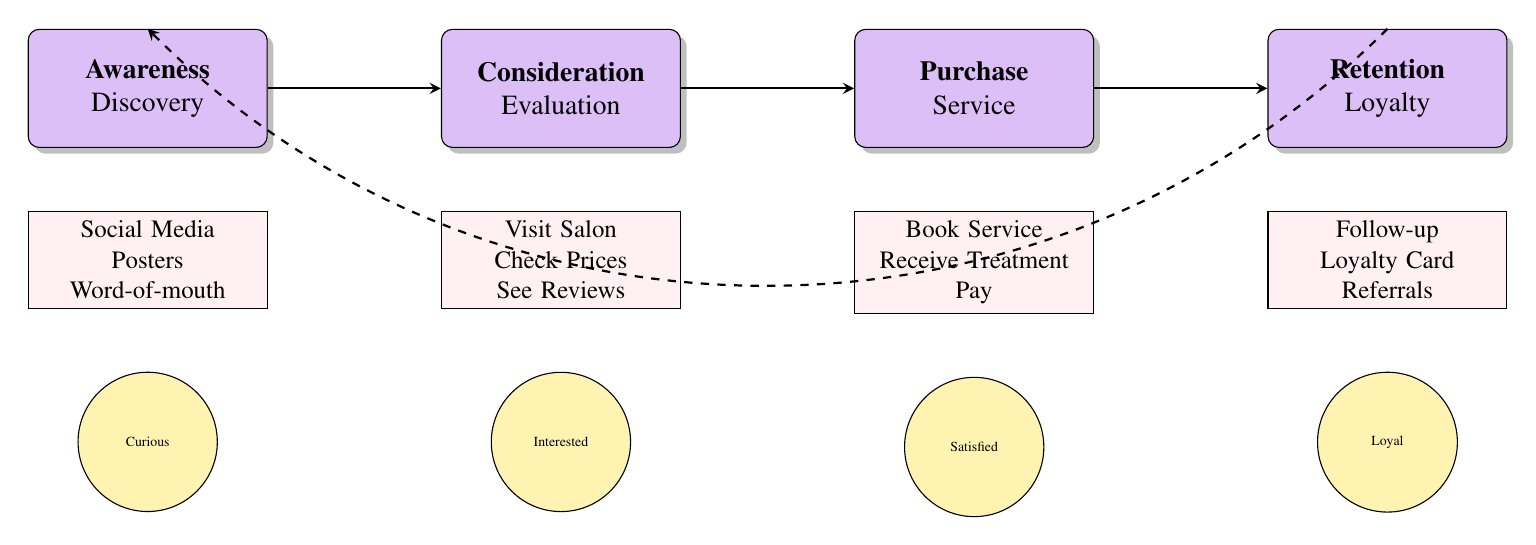
\begin{tikzpicture}[node distance=2.2cm, auto,
    stage/.style={rectangle, draw, fill=primarycolor!30, text width=2.8cm, text centered, rounded corners, minimum height=1.5cm, drop shadow},
    touchpoint/.style={rectangle, draw, fill=secondarycolor!20, text width=2.8cm, text centered, minimum height=0.8cm, font=\small},
    emotion/.style={circle, draw, fill=accentcolor!30, text width=1.5cm, text centered, font=\tiny},
    arrow/.style={->, >=stealth, thick}]
    
    % Journey stages
    \node [stage] (awareness) {\textbf{Awareness}\\Discovery};
    \node [stage, right=of awareness] (consideration) {\textbf{Consideration}\\Evaluation};
    \node [stage, right=of consideration] (purchase) {\textbf{Purchase}\\Service};
    \node [stage, right=of purchase] (retention) {\textbf{Retention}\\Loyalty};
    
    % Touchpoints
    \node [touchpoint, below=0.8cm of awareness] (t1) {Social Media\\Posters\\Word-of-mouth};
    \node [touchpoint, below=0.8cm of consideration] (t2) {Visit Salon\\Check Prices\\See Reviews};
    \node [touchpoint, below=0.8cm of purchase] (t3) {Book Service\\Receive Treatment\\Pay};
    \node [touchpoint, below=0.8cm of retention] (t4) {Follow-up\\Loyalty Card\\Referrals};
    
    % Emotions
    \node [emotion, below=0.8cm of t1] (e1) {Curious};
    \node [emotion, below=0.8cm of t2] (e2) {Interested};
    \node [emotion, below=0.8cm of t3] (e3) {Satisfied};
    \node [emotion, below=0.8cm of t4] (e4) {Loyal};
    
    % Arrows
    \draw [arrow] (awareness) -- (consideration);
    \draw [arrow] (consideration) -- (purchase);
    \draw [arrow] (purchase) -- (retention);
    \draw [arrow, dashed] (retention.north) to[bend left=45] (awareness.north);
    
\end{tikzpicture}

\vspace{0.5em}
Customer journey designed to convert awareness into loyalty through exceptional service experience.
\end{center}

\vspace{1em}

\begin{tcolorbox}[mybox, title=\textbf{Customer Journey Optimization}]
\textbf{Key Touchpoint Strategies:}
\begin{itemize}[leftmargin=1em, itemsep=0pt]
    \item \textbf{Awareness Stage:} Active social media presence, campus posters, student ambassadors
    \item \textbf{Consideration Stage:} Transparent pricing, visible quality standards, customer testimonials
    \item \textbf{Purchase Stage:} Easy booking, professional consultation, comfortable environment
    \item \textbf{Retention Stage:} Loyalty rewards, personalized follow-up, exclusive offers
\end{itemize}

\textbf{Reducing Friction Points:}
\begin{itemize}[leftmargin=1em, itemsep=0pt]
    \item No transport needed (on-campus location)
    \item Flexible payment options (cash, mobile money)
    \item Quick booking via WhatsApp
    \item Minimal waiting time
    \item Clear pricing with no hidden costs
\end{itemize}
\end{tcolorbox}

\subsection{Expected Sales Forecast}

\textbf{Month 1-3 (Launch Phase):}
\begin{itemize}[leftmargin=2em]
    \item Average daily customers: 3-5
    \item Average transaction value: UGX 18,000
    \item Monthly revenue: UGX 1,400,000-2,300,000
    \item Focus: Building awareness, establishing reputation, word-of-mouth marketing
\end{itemize}

\textbf{Month 4-6 (Growth Phase):}
\begin{itemize}[leftmargin=2em]
    \item Average daily customers: 6-8
    \item Average transaction value: UGX 20,000
    \item Monthly revenue: UGX 3,100,000-4,200,000
    \item Focus: Expanding customer base, loyalty program launch, repeat customers
\end{itemize}

\textbf{Month 7-12 (Established Phase):}
\begin{itemize}[leftmargin=2em]
    \item Average daily customers: 8-10
    \item Average transaction value: UGX 22,000
    \item Monthly revenue: UGX 4,600,000-5,700,000
    \item Focus: Steady operations, customer retention, service optimization
\end{itemize}

\textbf{Year 1 Total Projected Revenue:} UGX 40,000,000

\textbf{Sales Growth Projections:}
\begin{itemize}[leftmargin=2em]
    \item Year 1: UGX 40,000,000 (baseline - very conservative start)
    \item Year 2: UGX 70,000,000 (75\% growth as reputation builds)
    \item Year 3: UGX 105,000,000 (50\% growth)
    \item Year 4: UGX 145,000,000 (38\% growth)
    \item Year 5: UGX 190,000,000 (31\% growth)
\end{itemize}

\vspace{1em}

\begin{tcolorbox}[mybox, title=\textbf{Conservative Forecast Rationale}]
\textbf{Why Start with 3-5 Customers Daily?}
\begin{itemize}[leftmargin=1em, itemsep=0pt]
    \item \textbf{Ultra-Realistic Expectations:} New business needs time to build awareness
    \item \textbf{Quality Focus:} Very small numbers allow perfecting service delivery
    \item \textbf{Word-of-Mouth:} Each satisfied customer becomes an ambassador
    \item \textbf{Operational Learning:} Time to refine processes without overwhelming staff
    \item \textbf{Risk Mitigation:} Conservative projections reduce financial risk
\end{itemize}

\textbf{Growth Drivers:}
\begin{itemize}[leftmargin=1em, itemsep=0pt]
    \item Month 1-3: Initial customers + their referrals (3-5/day)
    \item Month 4-6: Repeat customers + expanded awareness (6-8/day)
    \item Month 7-12: Established reputation + loyalty program (8-10/day)
    \item Operating days: 26 days per month (closed Sundays)
    \item Average 7 customers/day across Year 1
\end{itemize}

\textbf{Market Penetration:}
\begin{itemize}[leftmargin=1em, itemsep=0pt]
    \item 7 customers/day × 26 days = 182 customers/month
    \item Total addressable market: 5,500 people
    \item Market penetration: Only 3.3\% (very achievable)
\end{itemize}
\end{tcolorbox}

\vspace{1em}

% Monthly Revenue Growth Chart
\begin{center}
\textbf{Year 1 Monthly Revenue Projection}
\vspace{0.5em}

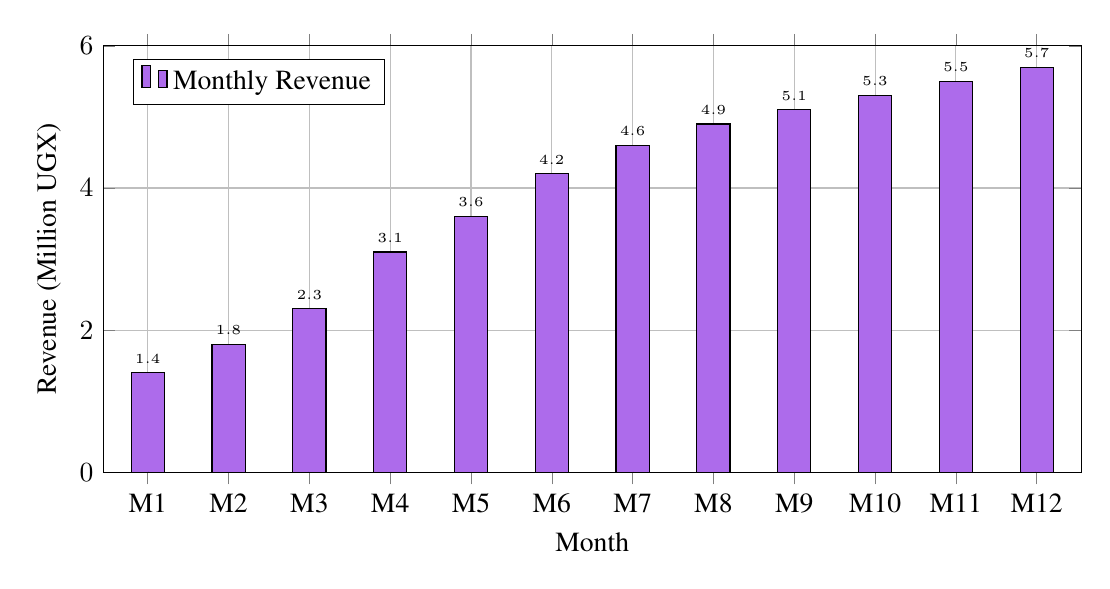
\begin{tikzpicture}
    \begin{axis}[
        ybar,
        bar width=12pt,
        xlabel={Month},
        ylabel={Revenue (Million UGX)},
        ymin=0,
        ymax=6,
        xtick=data,
        symbolic x coords={M1, M2, M3, M4, M5, M6, M7, M8, M9, M10, M11, M12},
        nodes near coords,
        nodes near coords style={font=\tiny},
        width=14cm,
        height=7cm,
        grid=major,
        ymajorgrids=true,
        enlarge x limits=0.05,
        legend pos=north west
    ]
    
    \addplot[fill=primarycolor!70] coordinates {
        (M1, 1.4) (M2, 1.8) (M3, 2.3) (M4, 3.1) (M5, 3.6) (M6, 4.2)
        (M7, 4.6) (M8, 4.9) (M9, 5.1) (M10, 5.3) (M11, 5.5) (M12, 5.7)
    };
    
    \legend{Monthly Revenue}
    
    % Add phase labels
    \draw[decorate, decoration={brace, amplitude=10pt, mirror}, thick] 
        (axis cs:M1,0) -- (axis cs:M3,0) node[midway, below=12pt, font=\small] {Launch (3-5/day)};
    \draw[decorate, decoration={brace, amplitude=10pt, mirror}, thick] 
        (axis cs:M4,0) -- (axis cs:M6,0) node[midway, below=12pt, font=\small] {Growth (6-8/day)};
    \draw[decorate, decoration={brace, amplitude=10pt, mirror}, thick] 
        (axis cs:M7,0) -- (axis cs:M12,0) node[midway, below=12pt, font=\small] {Established (8-10/day)};
    
    \end{axis}
\end{tikzpicture}

\vspace{0.5em}
Very conservative growth starting with 3-5 daily customers, building to 8-10 by year end.
\end{center}

\vspace{1em}

% 5-Year Revenue Projection
\begin{center}
\textbf{5-Year Revenue Growth Projection}
\vspace{0.5em}

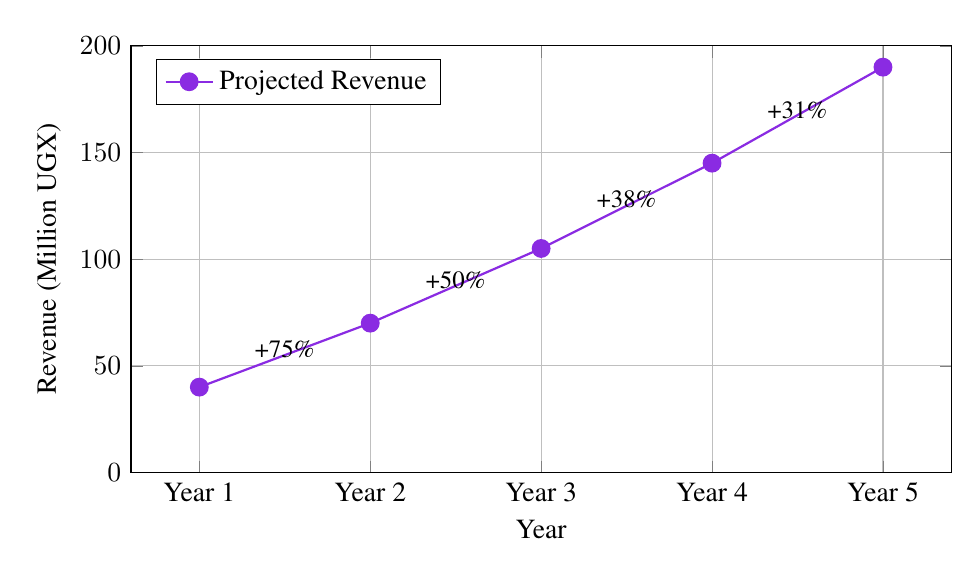
\begin{tikzpicture}
    \begin{axis}[
        xlabel={Year},
        ylabel={Revenue (Million UGX)},
        ymin=0,
        ymax=200,
        xtick={1,2,3,4,5},
        xticklabels={Year 1, Year 2, Year 3, Year 4, Year 5},
        width=12cm,
        height=7cm,
        grid=major,
        legend pos=north west,
        mark=*,
        mark size=3pt
    ]
    
    \addplot[color=primarycolor, thick, mark=*] coordinates {
        (1, 40) (2, 70) (3, 105) (4, 145) (5, 190)
    };
    
    % Add growth percentages
    \node at (axis cs:1.5,58) [font=\small] {+75\%};
    \node at (axis cs:2.5,90) [font=\small] {+50\%};
    \node at (axis cs:3.5,128) [font=\small] {+38\%};
    \node at (axis cs:4.5,170) [font=\small] {+31\%};
    
    \legend{Projected Revenue}
    
    \end{axis}
\end{tikzpicture}

\vspace{0.5em}
Strong growth trajectory after conservative Year 1, as business establishes reputation and customer base.
\end{center}

\vspace{1em}

% Customer Growth Chart
\begin{center}
\textbf{Daily Customer Growth Trajectory}
\vspace{0.5em}

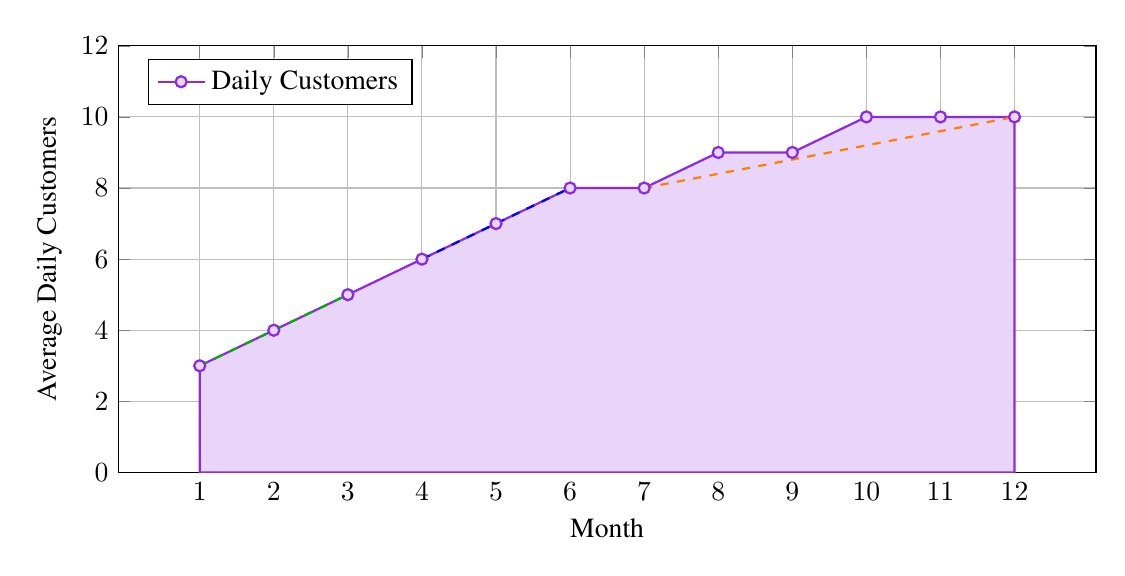
\begin{tikzpicture}
    \begin{axis}[
        xlabel={Month},
        ylabel={Average Daily Customers},
        ymin=0,
        ymax=12,
        xtick={1,2,3,4,5,6,7,8,9,10,11,12},
        width=14cm,
        height=7cm,
        grid=major,
        legend pos=north west,
        mark=*,
        mark size=2pt
    ]
    
    \addplot[color=primarycolor, thick, mark=*, fill=primarycolor!20] coordinates {
        (1,3) (2,4) (3,5) (4,6) (5,7) (6,8)
        (7,8) (8,9) (9,9) (10,10) (11,10) (12,10)
    } \closedcycle;
    
    \legend{Daily Customers}
    
    % Target zones
    \draw[dashed, thick, color=green!70!black] (axis cs:1,3) -- (axis cs:3,5);
    \draw[dashed, thick, color=blue] (axis cs:4,6) -- (axis cs:6,8);
    \draw[dashed, thick, color=orange] (axis cs:7,8) -- (axis cs:12,10);
    
    \end{axis}
\end{tikzpicture}

\vspace{0.5em}
Gradual customer growth from 3 to 10 daily customers over 12 months (average 7/day).
\end{center}

\subsection{Promotion Strategy}

\textbf{Comprehensive Integrated Marketing Communications Strategy:}

Campus Glam Hub will employ an integrated marketing communications approach that combines traditional and digital marketing channels to build brand awareness, attract customers, and foster loyalty. Our promotional strategy is specifically designed for the campus market, leveraging cost-effective channels that resonate with our target audience.

\vspace{1em}

\textbf{Marketing Objectives:}
\begin{itemize}[leftmargin=2em]
    \item Achieve 80\% brand awareness among target market within 6 months
    \item Generate 150-200 unique customers by Month 6
    \item Maintain customer acquisition cost below UGX 15,000 per customer
    \item Achieve 60\% customer retention rate in Year 1
    \item Build social media following of 2,000+ by end of Year 1
    \item Generate 40\% of new customers through referrals by Month 12
\end{itemize}

\vspace{1em}

\textbf{1. DIGITAL MARKETING STRATEGY}

\textbf{Social Media Marketing (Primary Channel - 60\% of marketing budget):}

\textbf{Instagram Strategy:}
\begin{itemize}[leftmargin=2em]
    \item \textbf{Content Mix:}
    \begin{itemize}
        \item Before/After transformations (40\%)
        \item Behind-the-scenes content (20\%)
        \item Customer testimonials and reviews (15\%)
        \item Educational content (hair care tips, makeup tutorials) (15\%)
        \item Promotional offers and announcements (10\%)
    \end{itemize}
    
    \item \textbf{Posting Schedule:}
    \begin{itemize}
        \item Feed posts: 1-2 times daily
        \item Stories: 3-5 times daily
        \item Reels: 3-4 times weekly
        \item IGTV tutorials: 1 time weekly
    \end{itemize}
    
    \item \textbf{Engagement Tactics:}
    \begin{itemize}
        \item Respond to all comments within 2 hours
        \item Host weekly Q\&A sessions
        \item Run monthly giveaways and contests
        \item Use relevant hashtags: \#MUSTBeauty \#CampusGlamHub \#MbararaBeauty
        \item Collaborate with campus influencers
        \item Feature customer photos (with permission)
    \end{itemize}
    
    \item \textbf{Instagram Advertising:}
    \begin{itemize}
        \item Budget: UGX 50,000 monthly
        \item Target: MUST students, 18-25 years, within 5km radius
        \item Ad Types: Story ads, feed ads, carousel ads
        \item Objectives: Brand awareness, traffic, conversions
    \end{itemize}
\end{itemize}

\textbf{Facebook Strategy:}
\begin{itemize}[leftmargin=2em]
    \item \textbf{Facebook Page Management:}
    \begin{itemize}
        \item Daily posts showcasing services and results
        \item Customer reviews and testimonials
        \item Event announcements and promotions
        \item Live videos of styling sessions
        \item Facebook Messenger for booking and inquiries
    \end{itemize}
    
    \item \textbf{Facebook Groups:}
    \begin{itemize}
        \item Join MUST student groups (10+ groups)
        \item Share valuable content, not just promotions
        \item Engage authentically with group members
        \item Offer exclusive group member discounts
    \end{itemize}
    
    \item \textbf{Facebook Advertising:}
    \begin{itemize}
        \item Budget: UGX 40,000 monthly
        \item Retargeting campaigns for website visitors
        \item Lookalike audiences based on customer database
        \item Event promotion ads for special occasions
    \end{itemize}
\end{itemize}

\textbf{TikTok Strategy:}
\begin{itemize}[leftmargin=2em]
    \item \textbf{Content Strategy:}
    \begin{itemize}
        \item Quick transformation videos (15-60 seconds)
        \item Trending audio with beauty content
        \item Hair and makeup tutorials
        \item Behind-the-scenes fun content
        \item Customer reactions and testimonials
    \end{itemize}
    
    \item \textbf{Posting Frequency:}
    \begin{itemize}
        \item 3-5 videos per week
        \item Post during peak hours (7-9 PM)
        \item Participate in trending challenges
    \end{itemize}
    
    \item \textbf{Growth Tactics:}
    \begin{itemize}
        \item Use trending sounds and hashtags
        \item Collaborate with campus TikTok creators
        \item Engage with comments and duets
        \item Cross-promote to Instagram Reels
    \end{itemize}
\end{itemize}

\textbf{WhatsApp Business:}
\begin{itemize}[leftmargin=2em]
    \item Professional business profile with services and pricing
    \item Automated greeting and away messages
    \item Quick replies for common questions
    \item Broadcast lists for promotions (with permission)
    \item Status updates showcasing daily work
    \item Booking confirmations and reminders
    \item Customer service and support
\end{itemize}

\textbf{Website and Online Presence:}
\begin{itemize}[leftmargin=2em]
    \item Simple, mobile-friendly website with:
    \begin{itemize}
        \item Service menu and pricing
        \item Photo gallery of work
        \item Online booking system
        \item Customer testimonials
        \item Contact information and location
        \item Blog with beauty tips
    \end{itemize}
    \item Google My Business listing
    \item Online review management (Google, Facebook)
\end{itemize}

\vspace{1em}

\textbf{2. TRADITIONAL MARKETING TACTICS}

\textbf{Campus Advertising (20\% of marketing budget):}

\textbf{Posters and Flyers:}
\begin{itemize}[leftmargin=2em]
    \item \textbf{Strategic Placement:}
    \begin{itemize}
        \item Notice boards in all faculty buildings
        \item Library notice boards
        \item Cafeteria and dining halls
        \item Hostel common areas
        \item Student center and guild offices
    \end{itemize}
    
    \item \textbf{Design Elements:}
    \begin{itemize}
        \item Eye-catching purple and pink brand colors
        \item Before/after photos
        \item Clear pricing and location information
        \item QR code linking to WhatsApp or Instagram
        \item Special offer or discount code
    \end{itemize}
    
    \item \textbf{Distribution Schedule:}
    \begin{itemize}
        \item New posters every 2 weeks
        \item Flyer distribution at start of semester
        \item Special event flyers for promotions
        \item Monthly refresh of all materials
    \end{itemize}
\end{itemize}

\textbf{Banners and Signage:}
\begin{itemize}[leftmargin=2em]
    \item Large banner at salon entrance
    \item Directional signs from main campus pathways
    \item A-frame sidewalk sign with daily specials
    \item Window graphics showcasing services
    \item Illuminated sign for evening visibility
\end{itemize}

\textbf{Campus Radio:}
\begin{itemize}[leftmargin=2em]
    \item Weekly 30-second spot advertisements
    \item Sponsorship of popular student shows
    \item Live mentions during peak listening hours
    \item Special promotion announcements
    \item Budget: UGX 20,000-30,000 monthly
\end{itemize}

\textbf{Print Materials:}
\begin{itemize}[leftmargin=2em]
    \item Professional business cards (1,000 units)
    \item Service menu cards
    \item Loyalty program cards
    \item Promotional vouchers
    \item Branded shopping bags for retail products
\end{itemize}

\vspace{1em}

\textbf{3. PUBLICITY AND PUBLIC RELATIONS}

\textbf{Grand Opening Event:}
\begin{itemize}[leftmargin=2em]
    \item \textbf{Event Details:}
    \begin{itemize}
        \item Date: First Saturday after opening
        \item Duration: 10 AM - 6 PM
        \item Location: Campus Glam Hub premises
    \end{itemize}
    
    \item \textbf{Activities:}
    \begin{itemize}
        \item Free mini-makeovers (first 50 customers)
        \item 30\% discount on all services
        \item Live demonstrations of styling techniques
        \item Raffle draw with prizes (free services, products)
        \item Refreshments and music
        \item Photo booth with branded backdrop
    \end{itemize}
    
    \item \textbf{Promotion:}
    \begin{itemize}
        \item Social media countdown (2 weeks before)
        \item Posters and flyers across campus
        \item Radio announcements
        \item Student organization partnerships
        \item Influencer invitations
    \end{itemize}
    
    \item \textbf{Budget:} UGX 500,000
\end{itemize}

\textbf{Strategic Partnerships:}
\begin{itemize}[leftmargin=2em]
    \item \textbf{Student Organizations:}
    \begin{itemize}
        \item Guild government: Official beauty partner
        \item Beauty pageant committees: Exclusive styling services
        \item Fashion clubs: Collaboration on events
        \item Sports teams: Team grooming packages
        \item Cultural groups: Event styling partnerships
    \end{itemize}
    
    \item \textbf{Partnership Benefits:}
    \begin{itemize}
        \item Exclusive member discounts (15-20\%)
        \item Sponsored services for organization events
        \item Co-branded promotional materials
        \item Cross-promotion on social media
        \item Priority booking for group events
    \end{itemize}
\end{itemize}

\textbf{Event Sponsorships:}
\begin{itemize}[leftmargin=2em]
    \item Campus beauty pageants (Miss MUST, Mr. MUST)
    \item Fashion shows and modeling competitions
    \item Graduation ceremonies (styling services)
    \item Sports events (team grooming)
    \item Cultural festivals and celebrations
    \item Budget: UGX 100,000-200,000 per event
\end{itemize}

\textbf{Media Relations:}
\begin{itemize}[leftmargin=2em]
    \item Press release for grand opening
    \item Features in campus newsletter
    \item Interviews on campus radio
    \item Articles in student publications
    \item Success stories and customer features
\end{itemize}

\textbf{Community Engagement:}
\begin{itemize}[leftmargin=2em]
    \item Free beauty workshops for students
    \item Career talks on beauty industry
    \item Internship opportunities for beauty students
    \item Charity events (free services for underprivileged)
    \item Environmental initiatives (eco-friendly products)
\end{itemize}

\vspace{1em}

\textbf{4. PROMOTIONAL CAMPAIGNS}

\textbf{Launch Campaign (Month 1):}
\begin{itemize}[leftmargin=2em]
    \item \textbf{Theme:} "Your Campus Beauty Destination is Here!"
    \item \textbf{Offers:}
    \begin{itemize}
        \item 25\% off all services for first 2 weeks
        \item Free deep conditioning with any haircut
        \item Buy 2 services, get 1 free (lowest price)
    \end{itemize}
    \item \textbf{Goal:} Generate initial customer base of 100+ customers
    \item \textbf{Budget:} UGX 200,000
\end{itemize}

\textbf{Student ID Discount Program (Ongoing):}
\begin{itemize}[leftmargin=2em]
    \item 10\% discount with valid MUST student ID
    \item Automatic application at checkout
    \item Promoted on all marketing materials
    \item Builds student loyalty and word-of-mouth
\end{itemize}

\textbf{Referral Program (Ongoing):}
\begin{itemize}[leftmargin=2em]
    \item \textbf{Program Name:} "Glam Friends Rewards"
    \item \textbf{Mechanics:}
    \begin{itemize}
        \item Refer a friend who books a service
        \item Both referrer and friend get 15\% off next service
        \item Unlimited referrals
        \item Track via unique referral codes
    \end{itemize}
    \item \textbf{Promotion:} Referral cards given after each service
    \item \textbf{Goal:} 40\% of new customers from referrals by Month 12
\end{itemize}

\textbf{Birthday Special Program (Ongoing):}
\begin{itemize}[leftmargin=2em]
    \item Free basic service during birthday month
    \item Options: Haircut, basic manicure, or eyebrow shaping
    \item Requires advance booking and ID verification
    \item Collect birthday information at first visit
    \item Automated WhatsApp birthday greetings
    \item Encourages annual visits and builds loyalty
\end{itemize}

\textbf{Loyalty Card Program (Ongoing):}
\begin{itemize}[leftmargin=2em]
    \item \textbf{Program Name:} "Glam Rewards Card"
    \item \textbf{Structure:}
    \begin{itemize}
        \item Collect stamps for each service
        \item 10 stamps = 50\% off next service
        \item 20 stamps = Free service (up to UGX 30,000 value)
        \item 50 stamps = VIP Gold status with permanent 15\% discount
    \end{itemize}
    \item \textbf{Card Design:} Branded physical card with stamp spaces
    \item \textbf{Digital Option:} Track via phone number in system
\end{itemize}

\textbf{Seasonal Campaigns:}

\textbf{Back to School Campaign (January, August):}
\begin{itemize}[leftmargin=2em]
    \item Theme: "Start the Semester Looking Fresh!"
    \item 20\% off all services for first 2 weeks
    \item Special student packages
    \item Social media contest: "New Semester, New Look"
    \item Budget: UGX 100,000
\end{itemize}

\textbf{Graduation Season Campaign (April-May, November-December):}
\begin{itemize}[leftmargin=2em]
    \item Theme: "Graduate in Style!"
    \item Graduation packages: Makeup + Hair + Nails
    \item Group booking discounts (3+ friends)
    \item Extended hours during graduation week
    \item Priority booking for graduates
    \item Budget: UGX 150,000
\end{itemize}

\textbf{Valentine's Day Campaign (February):}
\begin{itemize}[leftmargin=2em]
    \item Theme: "Love Yourself, Look Amazing!"
    \item Couples packages (his \& hers grooming)
    \item Special romantic styling options
    \item Valentine's makeup looks
    \item Social media photo contest
    \item Budget: UGX 80,000
\end{itemize}

\textbf{Exam Period Campaign (April, November):}
\begin{itemize}[leftmargin=2em]
    \item Theme: "Study Break Beauty Boost!"
    \item Express services for busy students
    \item 15\% discount on quick services
    \item Extended evening hours
    \item Stress-relief treatments (scalp massage, facials)
    \item Budget: UGX 60,000
\end{itemize}

\vspace{1em}

\textbf{5. WORD-OF-MOUTH MARKETING}

\textbf{Customer Experience Excellence:}
\begin{itemize}[leftmargin=2em]
    \item Exceed expectations to create brand advocates
    \item Personalized service and attention
    \item Remember customer preferences
    \item Follow-up messages after services
    \item Request reviews and testimonials
    \item Respond to all feedback promptly
\end{itemize}

\textbf{Student Ambassador Program:}
\begin{itemize}[leftmargin=2em]
    \item \textbf{Recruitment:} 10-15 popular students from different faculties
    \item \textbf{Benefits:}
    \begin{itemize}
        \item Free monthly service (up to UGX 25,000 value)
        \item 30\% discount on all other services
        \item Exclusive first access to new services
        \item Ambassador recognition on social media
    \end{itemize}
    \item \textbf{Responsibilities:}
    \begin{itemize}
        \item Share experiences on social media (2-3 posts monthly)
        \item Distribute promotional materials
        \item Provide referrals and recommendations
        \item Attend ambassador events and meetings
        \item Provide feedback on services and marketing
    \end{itemize}
    \item \textbf{Budget:} UGX 250,000 monthly (services + materials)
\end{itemize}

\textbf{Influencer Collaborations:}
\begin{itemize}[leftmargin=2em]
    \item Partner with 5-10 campus micro-influencers (500-5,000 followers)
    \item Offer free services in exchange for social media posts
    \item Authentic content showcasing real experiences
    \item Instagram stories, posts, and reels
    \item TikTok videos and reviews
    \item Budget: UGX 100,000 monthly (services + small fees)
\end{itemize}

\textbf{User-Generated Content:}
\begin{itemize}[leftmargin=2em]
    \item Encourage customers to share photos with branded hashtag
    \item Repost customer content (with permission)
    \item Monthly contest: Best customer photo wins free service
    \item Create shareable moments (photo backdrop, good lighting)
    \item Incentivize reviews with small discounts
\end{itemize}

\vspace{1em}

\textbf{6. MARKETING MIX (4Ps) SUMMARY}

\textbf{Product:}
\begin{itemize}[leftmargin=2em]
    \item High-quality beauty and grooming services
    \item Professional standards and trained staff
    \item Hygienic and comfortable environment
    \item Trendy styles and modern techniques
    \item Comprehensive service range
    \item Personalized consultations
    \item Quality retail products
\end{itemize}

\textbf{Price:}
\begin{itemize}[leftmargin=2em]
    \item Affordable, student-friendly pricing
    \item 15-20\% below town salon rates
    \item Value-added packages and bundles
    \item Transparent pricing with no hidden costs
    \item Multiple discount programs
    \item Flexible payment options (cash, mobile money)
\end{itemize}

\textbf{Place:}
\begin{itemize}[leftmargin=2em]
    \item Convenient on-campus location
    \item Accessible to all students and staff
    \item Comfortable and welcoming atmosphere
    \item Extended operating hours (8 AM - 8 PM)
    \item Professional salon environment
    \item Easy to find with clear signage
\end{itemize}

\textbf{Promotion:}
\begin{itemize}[leftmargin=2em]
    \item Active social media presence (Instagram, Facebook, TikTok)
    \item Word-of-mouth marketing through satisfied customers
    \item Strategic partnerships with student organizations
    \item Regular promotional campaigns and discounts
    \item Campus advertising (posters, flyers, radio)
    \item Event sponsorships and community engagement
    \item Influencer and ambassador programs
\end{itemize}

\vspace{1em}

\textbf{MARKETING BUDGET ALLOCATION}

\textbf{Monthly Marketing Budget: UGX 150,000}

\begin{itemize}[leftmargin=2em]
    \item Digital Marketing (60\%): UGX 90,000
    \begin{itemize}
        \item Social media advertising: UGX 50,000
        \item Content creation: UGX 20,000
        \item Website maintenance: UGX 10,000
        \item Influencer collaborations: UGX 10,000
    \end{itemize}
    
    \item Traditional Marketing (20\%): UGX 30,000
    \begin{itemize}
        \item Posters and flyers: UGX 15,000
        \item Campus radio: UGX 10,000
        \item Print materials: UGX 5,000
    \end{itemize}
    
    \item Promotions and Discounts (15\%): UGX 22,500
    \begin{itemize}
        \item Loyalty program costs: UGX 10,000
        \item Referral program rewards: UGX 7,500
        \item Birthday specials: UGX 5,000
    \end{itemize}
    
    \item Events and Partnerships (5\%): UGX 7,500
    \begin{itemize}
        \item Event sponsorships: UGX 5,000
        \item Partnership materials: UGX 2,500
    \end{itemize}
\end{itemize}

\textbf{First Year Marketing Budget: UGX 1,800,000}
\begin{itemize}[leftmargin=2em]
    \item Month 1 (Launch): UGX 500,000 (includes grand opening)
    \item Months 2-12: UGX 150,000 per month
    \item Special campaigns: UGX 390,000 (graduation, back-to-school, etc.)
\end{itemize}

\vspace{1em}

\begin{tcolorbox}[mybox, title=\textbf{Marketing Strategy Success Metrics}]
\textbf{Key Performance Indicators (KPIs):}
\begin{itemize}[leftmargin=1em, itemsep=0pt]
    \item \textbf{Brand Awareness:} 80\% of target market aware by Month 6
    \item \textbf{Customer Acquisition:} 150-200 unique customers by Month 6
    \item \textbf{Customer Acquisition Cost:} Below UGX 15,000 per customer
    \item \textbf{Social Media Following:} 2,000+ followers by end of Year 1
    \item \textbf{Engagement Rate:} 5-10\% on social media posts
    \item \textbf{Referral Rate:} 40\% of new customers from referrals by Month 12
    \item \textbf{Customer Retention:} 60\% retention rate in Year 1
    \item \textbf{Review Rating:} 4.5+ stars average on all platforms
\end{itemize}

\textbf{Marketing Competitive Advantages:}
\begin{itemize}[leftmargin=1em, itemsep=0pt]
    \item Student-focused messaging resonates with target market
    \item Cost-effective digital-first approach
    \item Strong word-of-mouth potential in close-knit campus community
    \item Strategic partnerships provide credibility and reach
    \item Authentic, relatable content vs. corporate salon marketing
    \item Agile, responsive to trends and feedback
\end{itemize}
\end{tcolorbox}

%---------------- Production and Operation Plan ----------------%
\newpage
\section{Production and Operation Plan}

\subsection{Product Development}

\textbf{Comprehensive Service Development Strategy:}

Campus Glam Hub is committed to continuous improvement and innovation in service offerings. Our product development approach balances customer needs, market trends, operational capabilities, and profitability considerations.

\subsubsection{Product Development Team}

\textbf{Core Development Team:}
\begin{itemize}[leftmargin=2em]
    \item \textbf{Namatovu Christine -- Owner \& Manager:}
    \begin{itemize}
        \item Overall business strategy and service development direction
        \item Market research and competitive analysis
        \item Financial viability assessment of new services
        \item Final approval on new service launches
        \item Customer feedback analysis and strategic response
    \end{itemize}
    
    \item \textbf{Lead Stylist -- Senior Beautician (5+ years experience):}
    \begin{itemize}
        \item Service quality standards and technique development
        \item Staff training program design and delivery
        \item New technique research and evaluation
        \item Product testing and quality assessment
        \item Industry trend monitoring and adaptation
        \item Technical feasibility assessment of new services
    \end{itemize}
    
    \item \textbf{Dr. Ruth Nakato -- Business Advisor:}
    \begin{itemize}
        \item Strategic guidance on business development
        \item Academic perspective on entrepreneurship
        \item Network connections and partnership opportunities
        \item Mentorship and advisory support
        \item Quarterly strategic review sessions
    \end{itemize}
    
    \item \textbf{Customer Feedback Team:}
    \begin{itemize}
        \item Regular customer surveys and feedback collection
        \item Analysis of customer preferences and requests
        \item Identification of service gaps and opportunities
        \item Monitoring of customer satisfaction metrics
        \item Reporting on customer insights to management
    \end{itemize}
    
    \item \textbf{All Staff Members:}
    \begin{itemize}
        \item Frontline insights on customer needs and preferences
        \item Suggestions for service improvements
        \item Participation in training and skill development
        \item Implementation of new services and techniques
    \end{itemize}
\end{itemize}

\textbf{Development Process:}
\begin{enumerate}[leftmargin=2em]
    \item \textbf{Idea Generation:} Customer feedback, staff suggestions, trend research, competitor analysis
    \item \textbf{Feasibility Assessment:} Technical capability, cost analysis, market demand, profitability projection
    \item \textbf{Pilot Testing:} Small-scale trial with select customers, feedback collection, refinement
    \item \textbf{Staff Training:} Comprehensive training on new service delivery, quality standards, safety protocols
    \item \textbf{Soft Launch:} Limited promotion to gauge response, monitor quality, gather feedback
    \item \textbf{Full Launch:} Complete marketing campaign, full menu integration, ongoing monitoring
    \item \textbf{Evaluation:} Performance review after 3 months, decision to continue, modify, or discontinue
\end{enumerate}

\subsubsection{Product Development Costs}

\textbf{Annual Development Budget: UGX 1,250,000-1,950,000}

\textbf{Detailed Cost Breakdown:}
\begin{itemize}[leftmargin=2em]
    \item \textbf{Staff Training Programs: UGX 500,000-800,000}
    \begin{itemize}
        \item Initial onboarding training: UGX 200,000
        \item Quarterly skill development workshops: UGX 150,000
        \item External training courses and certifications: UGX 200,000
        \item Online learning subscriptions: UGX 100,000
        \item Training materials and supplies: UGX 50,000
    \end{itemize}
    
    \item \textbf{New Technique Workshops: UGX 300,000-500,000}
    \begin{itemize}
        \item Industry expert workshops (2-3 annually): UGX 200,000
        \item Attendance at beauty trade shows: UGX 150,000
        \item Technique demonstration sessions: UGX 100,000
        \item Travel and accommodation for training: UGX 50,000
    \end{itemize}
    
    \item \textbf{Product Testing and Trials: UGX 200,000-300,000}
    \begin{itemize}
        \item Sample products for testing: UGX 150,000
        \item Trial services for feedback: UGX 80,000
        \item Product quality assessment: UGX 50,000
        \item Safety and allergy testing: UGX 20,000
    \end{itemize}
    
    \item \textbf{Customer Research and Surveys: UGX 100,000-200,000}
    \begin{itemize}
        \item Survey design and implementation: UGX 50,000
        \item Focus group sessions: UGX 80,000
        \item Data analysis and reporting: UGX 40,000
        \item Incentives for survey participants: UGX 30,000
    \end{itemize}
    
    \item \textbf{Service Menu Updates and Materials: UGX 150,000}
    \begin{itemize}
        \item Menu design and printing: UGX 80,000
        \item Marketing materials for new services: UGX 50,000
        \item Staff reference materials: UGX 20,000
    \end{itemize}
\end{itemize}

\textbf{Return on Investment:}
\begin{itemize}[leftmargin=2em]
    \item Improved service quality increases customer satisfaction and retention
    \item New services attract new customer segments and increase revenue
    \item Staff training reduces errors and improves efficiency
    \item Innovation maintains competitive advantage
    \item Expected ROI: 200-300\% over 2-3 years
\end{itemize}

\subsubsection{Product Development Risks and Mitigation}

\textbf{Risk 1: New Services Not Well-Received}
\begin{itemize}[leftmargin=2em]
    \item \textbf{Likelihood:} Medium
    \item \textbf{Impact:} Medium (wasted investment, disappointed customers)
    \item \textbf{Mitigation Strategies:}
    \begin{itemize}
        \item Conduct thorough market research before launch
        \item Start with pilot programs to test demand
        \item Offer introductory discounts to encourage trial
        \item Gather feedback and adjust quickly
        \item Have exit strategy to discontinue unsuccessful services
    \end{itemize}
\end{itemize}

\textbf{Risk 2: Training Costs Exceed Budget}
\begin{itemize}[leftmargin=2em]
    \item \textbf{Likelihood:} Low
    \item \textbf{Impact:} Medium (financial strain)
    \item \textbf{Mitigation Strategies:}
    \begin{itemize}
        \item Detailed budget planning with contingency
        \item Prioritize most critical training needs
        \item Seek free or low-cost training resources
        \item Negotiate group rates for training
        \item Spread training costs over time
    \end{itemize}
\end{itemize}

\textbf{Risk 3: Difficulty Finding Qualified Staff}
\begin{itemize}[leftmargin=2em]
    \item \textbf{Likelihood:} Medium
    \item \textbf{Impact:} High (service quality, expansion limitations)
    \item \textbf{Mitigation Strategies:}
    \begin{itemize}
        \item Build relationships with beauty training schools
        \item Offer competitive compensation and benefits
        \item Provide training to develop internal talent
        \item Maintain network of freelance professionals
        \item Start recruitment early for planned expansions
    \end{itemize}
\end{itemize}

\textbf{Risk 4: Product Allergies or Adverse Reactions}
\begin{itemize}[leftmargin=2em]
    \item \textbf{Likelihood:} Low
    \item \textbf{Impact:} High (customer harm, legal liability, reputation damage)
    \item \textbf{Mitigation Strategies:}
    \begin{itemize}
        \item Maintain comprehensive liability insurance
        \item Conduct patch tests for new products
        \item Use hypoallergenic products when possible
        \item Maintain detailed customer allergy records
        \item Have emergency response protocols
        \item Use only reputable, tested products
        \item Train staff on allergy recognition and response
    \end{itemize}
\end{itemize}

\textbf{Risk 5: Changing Trends Make Services Obsolete}
\begin{itemize}[leftmargin=2em]
    \item \textbf{Likelihood:} Medium
    \item \textbf{Impact:} Medium (reduced demand, wasted training)
    \item \textbf{Mitigation Strategies:}
    \begin{itemize}
        \item Continuous trend monitoring through social media
        \item Flexible service menu that can adapt quickly
        \item Focus on timeless services alongside trendy ones
        \item Regular staff training on emerging techniques
        \item Customer feedback on desired services
        \item Diversified service portfolio
    \end{itemize}
\end{itemize}

\textbf{Risk 6: Competition Copies Successful Innovations}
\begin{itemize}[leftmargin=2em]
    \item \textbf{Likelihood:} High
    \item \textbf{Impact:} Low (reduced competitive advantage)
    \item \textbf{Mitigation Strategies:}
    \begin{itemize}
        \item Build strong brand loyalty that transcends specific services
        \item Continuous innovation to stay ahead
        \item Focus on execution excellence, not just service offerings
        \item Protect unique processes where possible
        \item Emphasize overall customer experience
        \item Maintain first-mover advantage through speed
    \end{itemize}
\end{itemize}

\vspace{1em}

\textbf{Service Innovation Pipeline (Year 1-2):}
\begin{itemize}[leftmargin=2em]
    \item \textbf{Quarter 1-2:} Focus on core services, establish quality standards
    \item \textbf{Quarter 3:} Introduce express services for busy students
    \item \textbf{Quarter 4:} Launch men's grooming specialization
    \item \textbf{Year 2 Q1:} Add advanced skincare treatments
    \item \textbf{Year 2 Q2:} Introduce natural hair care specialization
    \item \textbf{Year 2 Q3:} Launch bridal package services
    \item \textbf{Year 2 Q4:} Add beauty workshops and training services
\end{itemize}

\subsection{Production Processes}

\textbf{Service Delivery Process:}

\begin{enumerate}[leftmargin=2em]
    \item \textbf{Customer Reception}
    \begin{itemize}
        \item Greet customer warmly
        \item Check for appointments or accept walk-ins
        \item Offer refreshments (water, tea)
        \item Estimated time: 2-3 minutes
    \end{itemize}
    
    \item \textbf{Consultation}
    \begin{itemize}
        \item Discuss desired service and style
        \item Assess hair/skin condition
        \item Recommend appropriate treatments
        \item Provide pricing information
        \item Estimated time: 5-10 minutes
    \end{itemize}
    
    \item \textbf{Service Preparation}
    \begin{itemize}
        \item Prepare workstation and tools
        \item Gather necessary products
        \item Ensure hygiene standards
        \item Estimated time: 3-5 minutes
    \end{itemize}
    
    \item \textbf{Service Delivery}
    \begin{itemize}
        \item Perform requested service professionally
        \item Maintain customer comfort
        \item Ensure quality standards
        \item Estimated time: 30 minutes-3 hours (depending on service)
    \end{itemize}
    
    \item \textbf{Quality Check}
    \begin{itemize}
        \item Review results with customer
        \item Make any necessary adjustments
        \item Provide aftercare advice
        \item Estimated time: 5-10 minutes
    \end{itemize}
    
    \item \textbf{Payment and Checkout}
    \begin{itemize}
        \item Process payment (cash or mobile money)
        \item Offer retail products
        \item Schedule next appointment if desired
        \item Thank customer and request feedback
        \item Estimated time: 5 minutes
    \end{itemize}
\end{enumerate}

\vspace{1em}

% Service Delivery Process Flowchart
\begin{center}
\textbf{Service Delivery Process Flowchart}
\vspace{0.5em}

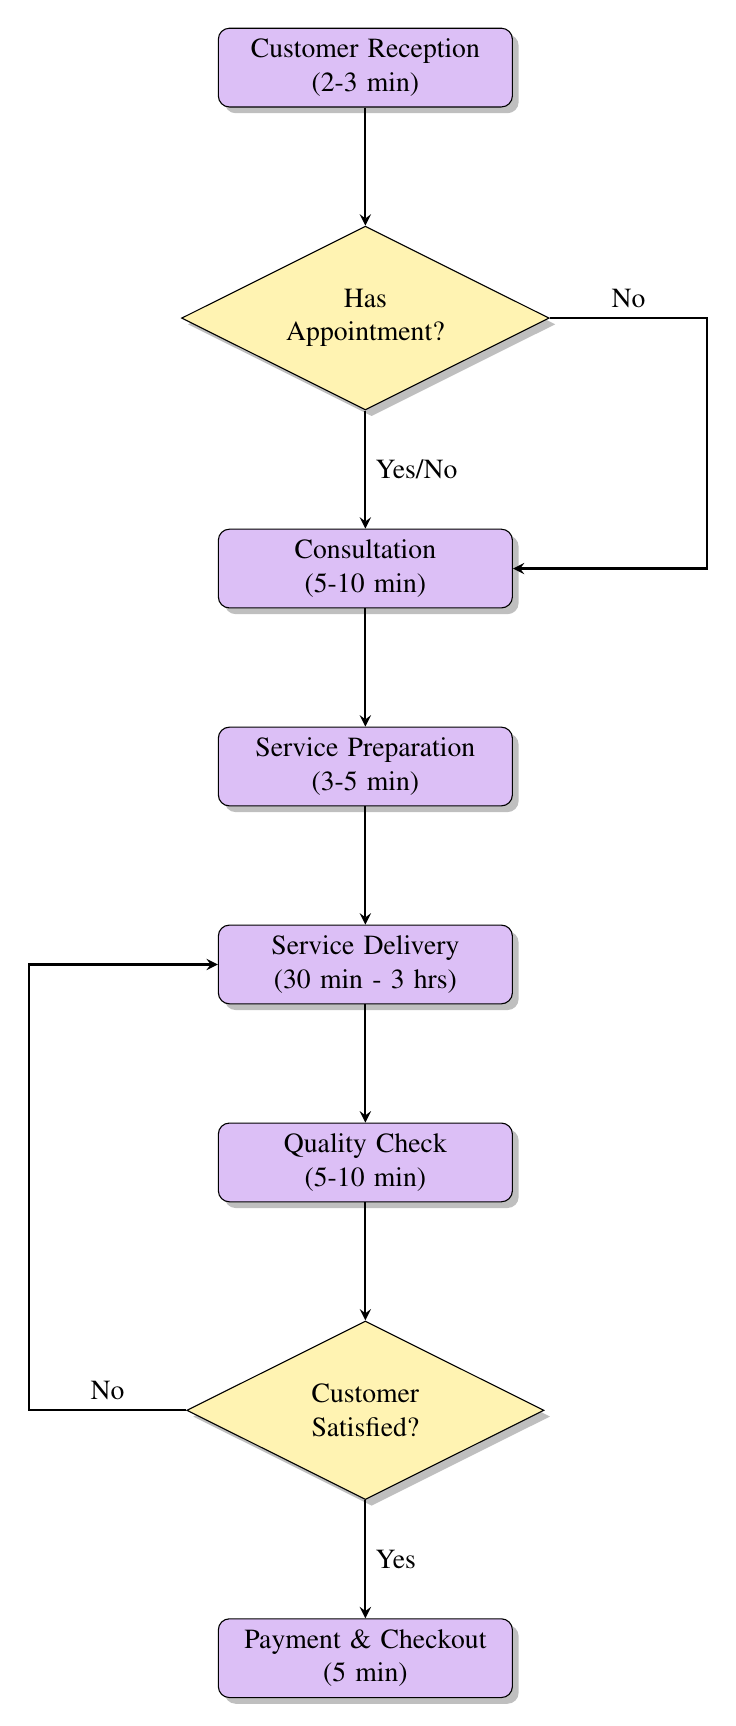
\begin{tikzpicture}[node distance=1.5cm, auto,
    process/.style={rectangle, draw, fill=primarycolor!30, text width=3.5cm, text centered, rounded corners, minimum height=1cm, drop shadow},
    decision/.style={diamond, draw, fill=accentcolor!30, text width=2.5cm, text centered, aspect=2, drop shadow},
    arrow/.style={->, >=stealth, thick}]
    
    % Nodes
    \node [process] (reception) {Customer Reception\\(2-3 min)};
    \node [decision, below=of reception] (appointment) {Has\\Appointment?};
    \node [process, below=of appointment] (consultation) {Consultation\\(5-10 min)};
    \node [process, below=of consultation] (preparation) {Service Preparation\\(3-5 min)};
    \node [process, below=of preparation] (service) {Service Delivery\\(30 min - 3 hrs)};
    \node [process, below=of service] (quality) {Quality Check\\(5-10 min)};
    \node [decision, below=of quality] (satisfied) {Customer\\Satisfied?};
    \node [process, below=of satisfied] (payment) {Payment \& Checkout\\(5 min)};
    
    % Arrows
    \draw [arrow] (reception) -- (appointment);
    \draw [arrow] (appointment) -- node[right] {Yes/No} (consultation);
    \draw [arrow] (consultation) -- (preparation);
    \draw [arrow] (preparation) -- (service);
    \draw [arrow] (service) -- (quality);
    \draw [arrow] (quality) -- (satisfied);
    \draw [arrow] (satisfied) -- node[right] {Yes} (payment);
    \draw [arrow] (satisfied.west) -- node[above] {No} ++(-2,0) |- (service.west);
    
    % Wait time for walk-ins
    \draw [arrow] (appointment.east) -- node[above] {No} ++(2,0) |- (consultation.east);
    
\end{tikzpicture}
\end{center}

\vspace{1em}

\begin{tcolorbox}[mybox, title=\textbf{Process Efficiency Measures}]
\textbf{Time Management:}
\begin{itemize}[leftmargin=1em, itemsep=0pt]
    \item Average service time: 45-90 minutes
    \item Maximum waiting time for walk-ins: 15 minutes
    \item Appointment slots: 30-minute intervals
    \item Buffer time between appointments: 10 minutes
\end{itemize}

\textbf{Quality Assurance at Each Step:}
\begin{itemize}[leftmargin=1em, itemsep=0pt]
    \item Reception: Warm greeting, professional appearance
    \item Consultation: Active listening, clear communication
    \item Preparation: Clean tools, organized workspace
    \item Service: Professional technique, customer comfort
    \item Quality Check: Customer satisfaction confirmation
    \item Checkout: Smooth payment, future booking encouragement
\end{itemize}
\end{tcolorbox}

\subsection{Production Equipment}

\textbf{Essential Equipment:}

\begin{itemize}[leftmargin=2em]
    \item \textbf{Hair Styling Equipment:}
    \begin{itemize}
        \item 4 salon chairs: UGX 800,000
        \item 4 styling stations with mirrors: UGX 1,200,000
        \item 2 hair dryers (standing): UGX 600,000
        \item 4 hand-held blow dryers: UGX 400,000
        \item Flat irons and curling irons: UGX 300,000
        \item Scissors, combs, brushes: UGX 200,000
    \end{itemize}
    
    \item \textbf{Washing and Treatment:}
    \begin{itemize}
        \item 2 shampoo bowls with chairs: UGX 1,000,000
        \item Hair steamer: UGX 400,000
        \item Towels and capes: UGX 150,000
    \end{itemize}
    
    \item \textbf{Makeup and Skincare:}
    \begin{itemize}
        \item Makeup station with lighting: UGX 500,000
        \item Facial steamer: UGX 300,000
        \item Makeup kits and brushes: UGX 400,000
        \item Skincare products: UGX 300,000
    \end{itemize}
    
    \item \textbf{Nail Services:}
    \begin{itemize}
        \item 2 manicure/pedicure stations: UGX 400,000
        \item Nail tools and equipment: UGX 200,000
        \item UV lamp for gel nails: UGX 150,000
    \end{itemize}
    
    \item \textbf{General Equipment:}
    \begin{itemize}
        \item Reception desk and chairs: UGX 300,000
        \item Waiting area furniture: UGX 400,000
        \item Storage cabinets: UGX 300,000
        \item Point of sale system: UGX 200,000
        \item Signage and branding: UGX 400,000
    \end{itemize}
\end{itemize}

\textbf{Total Equipment Investment:} UGX 8,000,000-9,000,000

\subsection{Quality Assurance}

\textbf{Quality Standards:}
\begin{itemize}[leftmargin=2em]
    \item All staff must complete professional training and certification
    \item Use of high-quality, reputable beauty products only
    \item Strict hygiene and sanitation protocols
    \item Regular equipment maintenance and cleaning
    \item Customer satisfaction surveys after each visit
    \item Minimum service time standards to ensure quality
\end{itemize}

\textbf{Quality Control Measures:}
\begin{itemize}[leftmargin=2em]
    \item Daily equipment inspection and cleaning
    \item Weekly inventory checks for product quality
    \item Monthly staff performance reviews
    \item Customer feedback monitoring and response system
    \item Mystery shopper evaluations quarterly
    \item Compliance with health and safety regulations
\end{itemize}

\textbf{Customer Satisfaction Guarantee:}
\begin{itemize}[leftmargin=2em]
    \item Free touch-ups within 48 hours if customer is unsatisfied
    \item Full refund policy for services not meeting standards
    \item Complaint resolution within 24 hours
    \item Regular customer appreciation events
\end{itemize}

\subsection{Administration}

\textbf{Administrative Structure:}
\begin{itemize}[leftmargin=2em]
    \item \textbf{Owner/Manager:} Overall business management, strategic decisions, financial oversight
    \item \textbf{Receptionist:} Customer service, appointment scheduling, payment processing
    \item \textbf{Lead Stylist:} Service quality supervision, staff training, inventory management
    \item \textbf{Accountant (Part-time):} Financial record keeping, tax compliance, reporting
\end{itemize}

\textbf{Administrative Processes:}
\begin{itemize}[leftmargin=2em]
    \item Daily sales and cash reconciliation
    \item Weekly inventory management and ordering
    \item Monthly financial reporting and analysis
    \item Quarterly performance reviews
    \item Annual business planning and budgeting
\end{itemize}

\textbf{Record Keeping:}
\begin{itemize}[leftmargin=2em]
    \item Customer database and appointment records
    \item Sales and revenue tracking
    \item Inventory and supply records
    \item Staff attendance and payroll records
    \item Financial statements and tax documents
\end{itemize}

\subsection{Key Suppliers of Inputs and Raw Materials}

\textbf{Primary Suppliers:}

\begin{enumerate}[leftmargin=2em]
    \item \textbf{Beauty Product Distributors in Kampala}
    \begin{itemize}
        \item Products: Hair care products, makeup, skincare items
        \item Delivery: Monthly bulk orders
        \item Payment terms: 30-day credit for established accounts
    \end{itemize}
    
    \item \textbf{Local Mbarara Beauty Supply Stores}
    \begin{itemize}
        \item Products: Emergency supplies, basic products
        \item Delivery: Same-day pickup
        \item Payment terms: Cash on delivery
    \end{itemize}
    
    \item \textbf{Equipment Suppliers}
    \begin{itemize}
        \item Products: Salon furniture, styling tools, equipment
        \item Delivery: One-time purchase with warranty
        \item Payment terms: 50\% deposit, 50\% on delivery
    \end{itemize}
    
    \item \textbf{Utility Providers}
    \begin{itemize}
        \item Water and electricity from campus utilities
        \item Internet service provider for business operations
        \item Payment terms: Monthly billing
    \end{itemize}
\end{enumerate}

\textbf{Supplier Management:}
\begin{itemize}[leftmargin=2em]
    \item Maintain relationships with multiple suppliers to ensure supply continuity
    \item Negotiate bulk purchase discounts
    \item Regular quality checks on supplied products
    \item Backup suppliers for critical items
\end{itemize}

\subsection{Product/Service Delivery}

\textbf{Service Delivery Standards:}
\begin{itemize}[leftmargin=2em]
    \item Maximum waiting time: 15 minutes for walk-ins
    \item Appointment punctuality: Services start within 5 minutes of scheduled time
    \item Service completion within estimated timeframe
    \item Professional and courteous staff interaction
    \item Clean and comfortable service environment
\end{itemize}

\textbf{Delivery Channels:}
\begin{itemize}[leftmargin=2em]
    \item In-salon services (primary channel)
    \item Appointment-based services for guaranteed time slots
    \item Express services for quick treatments during class breaks
    \item Group bookings for events and special occasions
\end{itemize}

\subsection{Customer Care}

\textbf{Customer Service Approach:}
\begin{itemize}[leftmargin=2em]
    \item Friendly, welcoming atmosphere from entry to exit
    \item Personalized consultations for each customer
    \item Active listening to customer preferences and concerns
    \item Professional advice on suitable styles and treatments
    \item Follow-up messages after services
    \item Responsive to complaints and feedback
\end{itemize}

\textbf{Customer Retention Strategies:}
\begin{itemize}[leftmargin=2em]
    \item Loyalty program with rewards
    \item Birthday and special occasion recognition
    \item Regular customer appreciation events
    \item Exclusive promotions for repeat customers
    \item Personalized service recommendations based on history
    \item Active engagement on social media
\end{itemize}

\textbf{Complaint Resolution:}
\begin{itemize}[leftmargin=2em]
    \item Immediate acknowledgment of complaints
    \item Investigation and resolution within 24 hours
    \item Compensation or corrective services as appropriate
    \item Follow-up to ensure satisfaction
    \item Documentation of complaints for continuous improvement
\end{itemize}

\subsection{Human Resource Plan}

\textbf{Staffing Requirements:}

\begin{enumerate}[leftmargin=2em]
    \item \textbf{Owner/Manager (1)} -- Namatovu Christine
    \begin{itemize}
        \item Responsibilities: Overall management, strategic planning, financial oversight
        \item Qualifications: Business management knowledge, entrepreneurial skills
        \item Compensation: Profit share
    \end{itemize}
    
    \item \textbf{Lead Stylist (1)}
    \begin{itemize}
        \item Responsibilities: Hair services, staff supervision, quality control
        \item Qualifications: 5+ years experience, professional certification
        \item Salary: UGX 400,000-500,000 per month
    \end{itemize}
    
    \item \textbf{Beautician/Makeup Artist (1)}
    \begin{itemize}
        \item Responsibilities: Makeup, skincare, nail services
        \item Qualifications: 3+ years experience, professional training
        \item Salary: UGX 300,000-400,000 per month
    \end{itemize}
    
    \item \textbf{Junior Stylist (1)}
    \begin{itemize}
        \item Responsibilities: Assist with services, basic styling, cleaning
        \item Qualifications: 1-2 years experience or recent graduate
        \item Salary: UGX 200,000-250,000 per month
    \end{itemize}
    
    \item \textbf{Receptionist (1)}
    \begin{itemize}
        \item Responsibilities: Customer service, appointments, payments, basic admin
        \item Qualifications: Good communication skills, basic computer literacy
        \item Salary: UGX 200,000-250,000 per month
    \end{itemize}
\end{enumerate}

\textbf{Total Monthly Payroll:} UGX 1,100,000-1,400,000

\textbf{Personnel Plan:}
\begin{itemize}[leftmargin=2em]
    \item \textbf{Recruitment:} Advertise positions through university networks, beauty schools, and online platforms
    \item \textbf{Training:} 2-week onboarding program covering service standards, customer care, and safety protocols
    \item \textbf{Development:} Quarterly training workshops on new techniques and trends
    \item \textbf{Performance Management:} Monthly reviews with feedback and goal setting
    \item \textbf{Retention:} Competitive salaries, performance bonuses, positive work environment
    \item \textbf{Benefits:} Health insurance contribution, paid leave, staff discounts on services
\end{itemize}

\subsection{Facilities}

\textbf{Location:} Kihumuro Campus, Mbarara University of Science and Technology

\textbf{Space Requirements:}
\begin{itemize}[leftmargin=2em]
    \item Total space: 60-80 square meters
    \item Reception area: 10 square meters
    \item Hair styling area: 25 square meters
    \item Makeup and skincare area: 15 square meters
    \item Nail services area: 10 square meters
    \item Storage and supplies: 8 square meters
    \item Staff room and restroom: 10 square meters
\end{itemize}

\textbf{Facility Features:}
\begin{itemize}[leftmargin=2em]
    \item Well-lit with natural and artificial lighting
    \item Proper ventilation and air circulation
    \item Running water and drainage
    \item Reliable electricity supply
    \item Comfortable temperature control
    \item Clean and hygienic environment
    \item Attractive interior design and branding
    \item Accessible location with good visibility
\end{itemize}

\textbf{Facility Costs:}
\begin{itemize}[leftmargin=2em]
    \item Monthly rent: UGX 400,000-600,000
    \item Initial renovation and setup: UGX 2,000,000-3,000,000
    \item Utilities (water, electricity): UGX 150,000-200,000 per month
    \item Internet: UGX 100,000 per month
    \item Maintenance: UGX 50,000-100,000 per month
\end{itemize}

\vspace{1em}

% Facility Layout Diagram
\begin{center}
\textbf{Campus Glam Hub Facility Layout (70 sqm)}
\vspace{0.5em}

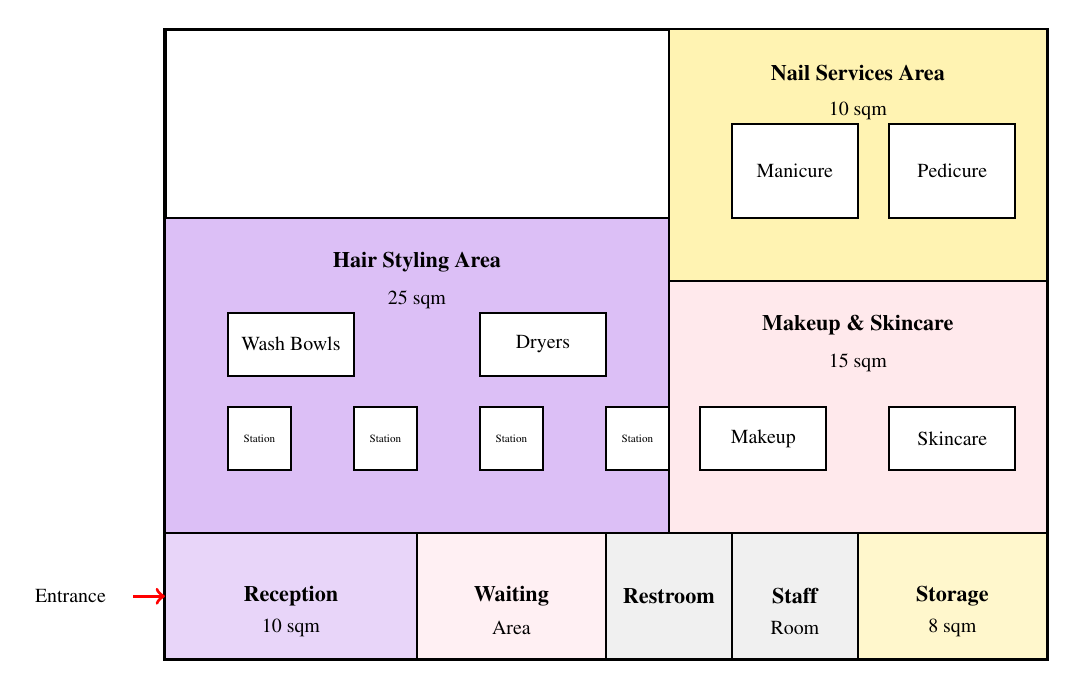
\begin{tikzpicture}[scale=0.8, transform shape]
    % Outer boundary
    \draw[very thick] (0,0) rectangle (14,10);
    
    % Reception (bottom)
    \draw[fill=primarycolor!20, thick] (0,0) rectangle (4,2);
    \node at (2,1) {\textbf{Reception}};
    \node at (2,0.5) [font=\small] {10 sqm};
    
    % Waiting Area
    \draw[fill=secondarycolor!20, thick] (4,0) rectangle (7,2);
    \node at (5.5,1) {\textbf{Waiting}};
    \node at (5.5,0.5) [font=\small] {Area};
    
    % Restroom
    \draw[fill=lightgray, thick] (7,0) rectangle (9,2);
    \node at (8,1) {\textbf{Restroom}};
    
    % Staff Room
    \draw[fill=lightgray, thick] (9,0) rectangle (11,2);
    \node at (10,1) {\textbf{Staff}};
    \node at (10,0.5) [font=\small] {Room};
    
    % Storage
    \draw[fill=accentcolor!20, thick] (11,0) rectangle (14,2);
    \node at (12.5,1) {\textbf{Storage}};
    \node at (12.5,0.5) [font=\small] {8 sqm};
    
    % Hair Styling Area (large central area)
    \draw[fill=primarycolor!30, thick] (0,2) rectangle (8,7);
    \node at (4,6.3) {\textbf{Hair Styling Area}};
    \node at (4,5.7) [font=\small] {25 sqm};
    
    % Draw 4 styling stations
    \foreach \x in {1,3,5,7} {
        \draw[fill=white, thick] (\x,3) rectangle (\x+1,4);
        \node at (\x+0.5,3.5) [font=\tiny] {Station};
    }
    
    % Shampoo area
    \draw[fill=white, thick] (1,4.5) rectangle (3,5.5);
    \node at (2,5) [font=\small] {Wash Bowls};
    
    % Dryers
    \draw[fill=white, thick] (5,4.5) rectangle (7,5.5);
    \node at (6,5) [font=\small] {Dryers};
    
    % Makeup and Skincare Area
    \draw[fill=secondarycolor!30, thick] (8,2) rectangle (14,6);
    \node at (11,5.3) {\textbf{Makeup \& Skincare}};
    \node at (11,4.7) [font=\small] {15 sqm};
    
    % Makeup stations
    \draw[fill=white, thick] (8.5,3) rectangle (10.5,4);
    \node at (9.5,3.5) [font=\small] {Makeup};
    \draw[fill=white, thick] (11.5,3) rectangle (13.5,4);
    \node at (12.5,3.5) [font=\small] {Skincare};
    
    % Nail Services Area
    \draw[fill=accentcolor!30, thick] (8,6) rectangle (14,10);
    \node at (11,9.3) {\textbf{Nail Services Area}};
    \node at (11,8.7) [font=\small] {10 sqm};
    
    % Nail stations
    \draw[fill=white, thick] (9,7) rectangle (11,8.5);
    \node at (10,7.75) [font=\small] {Manicure};
    \draw[fill=white, thick] (11.5,7) rectangle (13.5,8.5);
    \node at (12.5,7.75) [font=\small] {Pedicure};
    
    % Entrance arrow
    \draw[->, very thick, color=red] (-0.5,1) -- (0,1);
    \node at (-1.5,1) [font=\small] {Entrance};
    
\end{tikzpicture}

\vspace{0.5em}
Efficient layout maximizes space utilization while ensuring customer comfort and workflow efficiency.
\end{center}

\vspace{1em}

\begin{tcolorbox}[mybox, title=\textbf{Facility Design Principles}]
\textbf{Layout Optimization:}
\begin{itemize}[leftmargin=1em, itemsep=0pt]
    \item \textbf{Customer Flow:} Reception → Service Area → Checkout (smooth progression)
    \item \textbf{Privacy:} Separate areas for different services
    \item \textbf{Efficiency:} Staff can move easily between stations
    \item \textbf{Comfort:} Adequate space prevents crowding
    \item \textbf{Hygiene:} Separate storage and staff areas
\end{itemize}

\textbf{Ambiance Elements:}
\begin{itemize}[leftmargin=1em, itemsep=0pt]
    \item Soft background music for relaxation
    \item Pleasant lighting (natural + warm artificial)
    \item Comfortable seating in waiting area
    \item Branded decor in purple and pink tones
    \item Fresh, clean scent throughout
    \item Mirrors strategically placed for customer viewing
\end{itemize}
\end{tcolorbox}

%---------------- Management and Organization Plan ----------------%
\newpage
\section{Management and Organization Plan}

\subsection{Management Team}

\textbf{Namatovu Christine -- Owner \& Manager}
\begin{itemize}[leftmargin=2em]
    \item Education: Bachelor of Science in Computer Science (in progress), Mbarara University
    \item Role: Overall business strategy, financial management, operations oversight
    \item Responsibilities:
    \begin{itemize}
        \item Strategic planning and business development
        \item Financial management and budgeting
        \item Marketing and brand development
        \item Supplier relationships and negotiations
        \item Staff recruitment and management
        \item Compliance with regulations
    \end{itemize}
    \item Time commitment: Full-time
\end{itemize}

\textbf{Dr. Ruth Nakato -- Business Advisor}
\begin{itemize}[leftmargin=2em]
    \item Education: PhD, Lecturer at Mbarara University
    \item Role: Strategic advisor and mentor
    \item Responsibilities:
    \begin{itemize}
        \item Provide business guidance and mentorship
        \item Review business strategies and plans
        \item Offer academic and professional insights
        \item Connect business with university resources
    \end{itemize}
    \item Time commitment: Advisory (as needed)
\end{itemize}

\subsection{Board of Directors}

As a small startup business, Campus Glam Hub will initially operate without a formal board of directors. However, an advisory board will be established consisting of:

\begin{itemize}[leftmargin=2em]
    \item \textbf{Dr. Ruth Nakato} -- Business and Academic Advisor
    \item \textbf{Beauty Industry Professional} -- Technical advisor (to be appointed)
    \item \textbf{Financial Advisor} -- Accountant or financial consultant (to be appointed)
\end{itemize}

As the business grows, a formal board may be established to provide governance and strategic oversight.

\subsection{Staffing}

\textbf{Current Staffing Plan (Year 1):}

\begin{tabular}{|l|l|l|}
\hline
\textbf{Position} & \textbf{Number} & \textbf{Monthly Salary (UGX)} \\
\hline
Owner/Manager & 1 & Profit share \\
Lead Stylist & 1 & 400,000-500,000 \\
Beautician/Makeup Artist & 1 & 300,000-400,000 \\
Junior Stylist & 1 & 200,000-250,000 \\
Receptionist & 1 & 200,000-250,000 \\
\hline
\textbf{Total} & \textbf{5} & \textbf{1,100,000-1,400,000} \\
\hline
\end{tabular}

\vspace{1em}

\textbf{Future Staffing Expansion (Year 2-3):}
\begin{itemize}[leftmargin=2em]
    \item Additional stylist (Year 2)
    \item Marketing coordinator (Year 2)
    \item Additional beautician (Year 3)
    \item Assistant manager (Year 3)
\end{itemize}

\subsection{Personnel Plan}

\textbf{Recruitment Strategy:}
\begin{itemize}[leftmargin=2em]
    \item Advertise through beauty schools and training institutes
    \item Post on university job boards and student networks
    \item Use social media and online job platforms
    \item Seek referrals from industry professionals
    \item Conduct thorough interviews and practical assessments
\end{itemize}

\textbf{Training and Development:}
\begin{itemize}[leftmargin=2em]
    \item Initial 2-week orientation and training program
    \item Monthly team meetings for updates and feedback
    \item Quarterly skills development workshops
    \item Annual attendance at beauty industry conferences or trade shows
    \item Cross-training to ensure service continuity
\end{itemize}

\textbf{Compensation and Benefits:}
\begin{itemize}[leftmargin=2em]
    \item Competitive base salaries
    \item Performance-based bonuses (5-10\% of salary)
    \item Commission on retail product sales (10\%)
    \item Staff discounts on services (50\% off)
    \item Contribution to health insurance
    \item Paid annual leave (15 days)
    \item Sick leave (10 days)
    \item Professional development support
\end{itemize}

\textbf{Performance Management:}
\begin{itemize}[leftmargin=2em]
    \item Monthly one-on-one performance reviews
    \item Customer satisfaction scores as key metric
    \item Service quality assessments
    \item Attendance and punctuality tracking
    \item Annual comprehensive performance evaluation
    \item Clear promotion pathways
\end{itemize}

\subsection{Organizational Chart}

\begin{center}
\textbf{Campus Glam Hub Organizational Structure}
\vspace{0.5em}

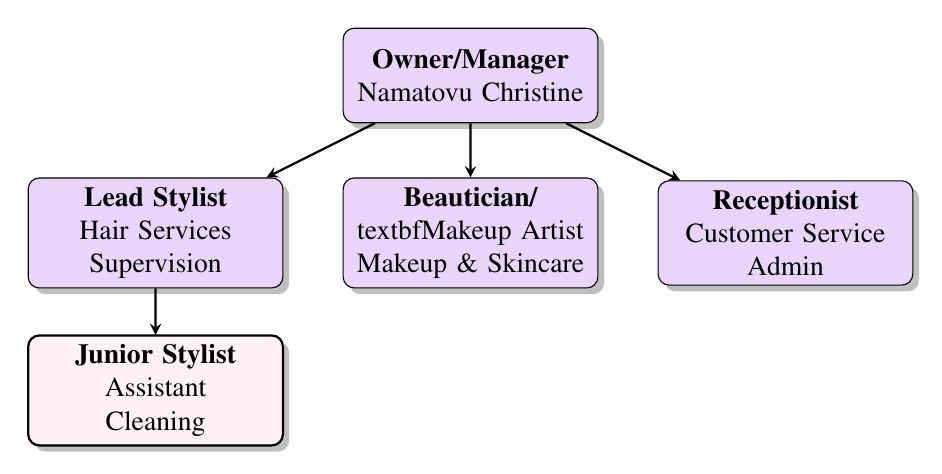
\begin{tikzpicture}[
    level 1/.style={sibling distance=4cm, level distance=2cm},
    level 2/.style={sibling distance=3cm, level distance=2cm},
    every node/.style={rectangle, draw, rounded corners, fill=primarycolor!20, 
                       text width=3cm, text centered, minimum height=1.2cm, drop shadow},
    edge from parent/.style={draw, ->, >=stealth, thick}
]

\node {\textbf{Owner/Manager}\\Namatovu Christine}
    child {node {\textbf{Lead Stylist}\\Hair Services\\Supervision}
        child {node[fill=secondarycolor!20] {\textbf{Junior Stylist}\\Assistant\\Cleaning}}
    }
    child {node {\textbf{Beautician/}\\textbf{Makeup Artist}\\Makeup \& Skincare}}
    child {node {\textbf{Receptionist}\\Customer Service\\Admin}};

\end{tikzpicture}
\end{center}

\vspace{1em}

% Advisory Board
\begin{center}
\textbf{Advisory Support Structure}
\vspace{0.5em}

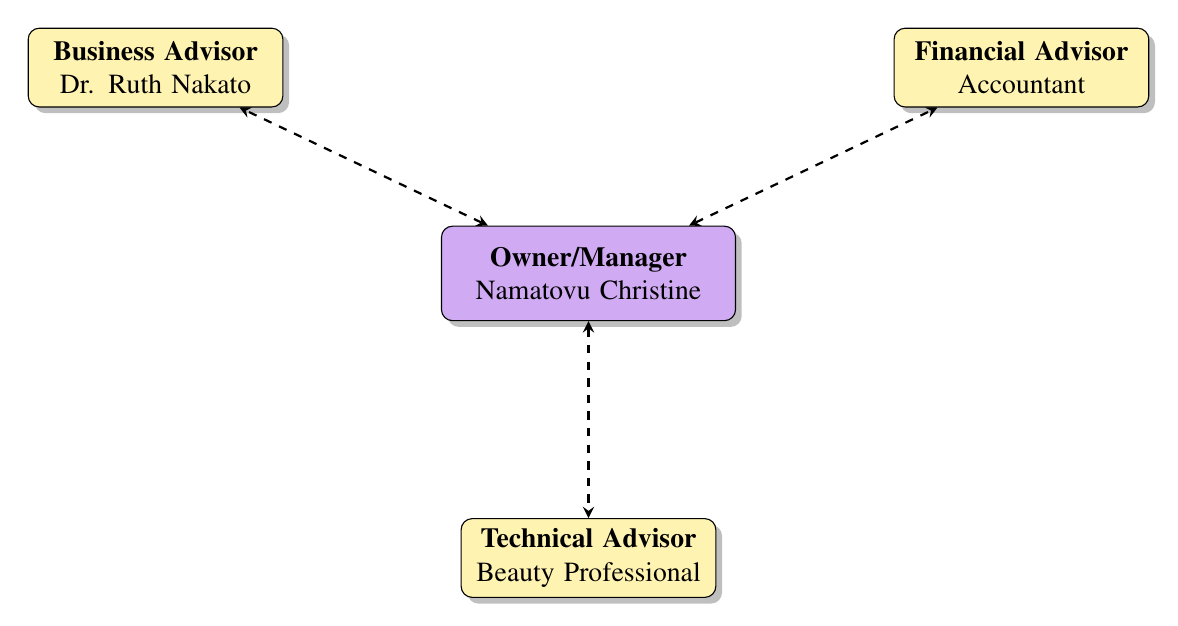
\begin{tikzpicture}[node distance=2.5cm, auto,
    advisor/.style={rectangle, draw, fill=accentcolor!30, text width=3cm, text centered, rounded corners, minimum height=1cm, drop shadow},
    manager/.style={rectangle, draw, fill=primarycolor!40, text width=3.5cm, text centered, rounded corners, minimum height=1.2cm, drop shadow},
    arrow/.style={<->, >=stealth, thick, dashed}]
    
    \node [manager] (manager) {\textbf{Owner/Manager}\\Namatovu Christine};
    \node [advisor, above left=1.5cm and 2cm of manager] (business) {\textbf{Business Advisor}\\Dr. Ruth Nakato};
    \node [advisor, above right=1.5cm and 2cm of manager] (financial) {\textbf{Financial Advisor}\\Accountant};
    \node [advisor, below=of manager] (technical) {\textbf{Technical Advisor}\\Beauty Professional};
    
    \draw [arrow] (manager) -- (business);
    \draw [arrow] (manager) -- (financial);
    \draw [arrow] (manager) -- (technical);
    
\end{tikzpicture}
\end{center}

\vspace{1em}

\textbf{Reporting Structure:}
\begin{itemize}[leftmargin=2em]
    \item All staff report directly to the Owner/Manager
    \item Lead Stylist supervises Junior Stylist
    \item Lead Stylist coordinates with Beautician/Makeup Artist on service scheduling
    \item Receptionist coordinates with all service staff for appointments
\end{itemize}

\textbf{Advisory Support:}
\begin{itemize}[leftmargin=2em]
    \item Dr. Ruth Nakato provides strategic business advice to Owner/Manager
    \item External accountant provides financial guidance
    \item Industry professionals provide technical consultation as needed
\end{itemize}

\vspace{1em}

\begin{tcolorbox}[mybox, title=\textbf{Organizational Design Rationale}]
\textbf{Flat Structure Benefits:}
\begin{itemize}[leftmargin=1em, itemsep=0pt]
    \item Quick decision-making and communication
    \item Direct owner involvement ensures quality
    \item Flexible team that can adapt to demand
    \item Lower overhead costs
    \item Strong team cohesion
\end{itemize}

\textbf{Scalability Plan:}
\begin{itemize}[leftmargin=1em, itemsep=0pt]
    \item Year 2: Add Assistant Manager role
    \item Year 2: Hire additional stylist
    \item Year 3: Create Marketing Coordinator position
    \item Year 3: Expand to second location (if successful)
\end{itemize}
\end{tcolorbox}

%---------------- Financial Plan ----------------%
\newpage
\section{Financial Plan}

\subsection{Financial Requirements}

\textbf{Startup Capital Requirements:}

\begin{tabular}{|l|r|}
\hline
\textbf{Item} & \textbf{Amount (UGX)} \\
\hline
Equipment and furniture & 8,500,000 \\
Initial inventory (products) & 1,500,000 \\
Facility renovation and setup & 2,500,000 \\
Signage and branding & 400,000 \\
Business registration and licenses & 300,000 \\
Initial marketing campaign & 500,000 \\
Working capital (3 months) & 3,000,000 \\
Contingency fund (10\%) & 1,670,000 \\
\hline
\textbf{Total Startup Capital} & \textbf{18,370,000} \\
\hline
\end{tabular}

\vspace{1em}

% Startup Capital Breakdown Chart
\begin{center}
\textbf{Startup Capital Allocation}
\vspace{0.5em}

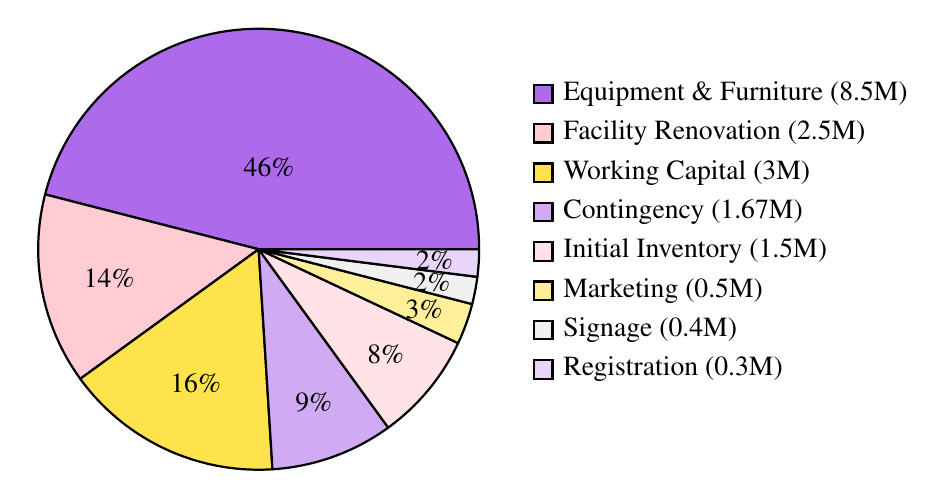
\begin{tikzpicture}
    \pie[
        text=legend,
        radius=2.8,
        color={primarycolor!70, secondarycolor!70, accentcolor!70, 
               primarycolor!40, secondarycolor!40, accentcolor!40, 
               lightgray, primarycolor!20}
    ]{
        46/Equipment \& Furniture (8.5M),
        14/Facility Renovation (2.5M),
        16/Working Capital (3M),
        9/Contingency (1.67M),
        8/Initial Inventory (1.5M),
        3/Marketing (0.5M),
        2/Signage (0.4M),
        2/Registration (0.3M)
    }
\end{tikzpicture}
\end{center}

\vspace{1em}

\textbf{Monthly Operating Expenses:}

\begin{tabular}{|l|r|}
\hline
\textbf{Expense Category} & \textbf{Amount (UGX)} \\
\hline
Rent & 500,000 \\
Staff salaries & 1,300,000 \\
Products and supplies & 400,000 \\
Utilities (water, electricity) & 180,000 \\
Internet and phone & 100,000 \\
Marketing & 150,000 \\
Maintenance and repairs & 80,000 \\
Insurance & 50,000 \\
Miscellaneous & 100,000 \\
\hline
\textbf{Total Monthly Expenses} & \textbf{2,860,000} \\
\hline
\end{tabular}

\vspace{1em}

% Monthly Operating Expenses Chart
\begin{center}
\textbf{Monthly Operating Expenses Breakdown}
\vspace{0.5em}

\begin{tikzpicture}
    \begin{axis}[
        xbar,
        width=12cm,
        height=8cm,
        xlabel={Amount (Million UGX)},
        symbolic y coords={Miscellaneous, Insurance, Maintenance, Marketing, 
                          Internet, Utilities, Products, Rent, Salaries},
        ytick=data,
        nodes near coords,
        nodes near coords align={horizontal},
        xmin=0,
        xmax=1.5,
        bar width=15pt,
        enlarge y limits=0.1
    ]
    
    \addplot[fill=primarycolor!70] coordinates {
        (0.1, Miscellaneous)
        (0.05, Insurance)
        (0.08, Maintenance)
        (0.15, Marketing)
        (0.1, Internet)
        (0.18, Utilities)
        (0.4, Products)
        (0.5, Rent)
        (1.3, Salaries)
    };
    
    \end{axis}
\end{tikzpicture}

\vspace{0.5em}
Staff salaries represent the largest operating expense at 45\% of monthly costs.
\end{center}

\subsection{Financing Strategy}

\textbf{Funding Sources:}
\begin{itemize}[leftmargin=2em]
    \item \textbf{Personal Savings:} UGX 5,000,000 (27\%)
    \item \textbf{Family Contribution:} UGX 3,000,000 (16\%)
    \item \textbf{Bank Loan:} UGX 8,000,000 (44\%)
    \item \textbf{Youth/Student Grant:} UGX 2,370,000 (13\%)
    \item \textbf{Total:} UGX 18,370,000
\end{itemize}

\textbf{Loan Terms (if applicable):}
\begin{itemize}[leftmargin=2em]
    \item Loan amount: UGX 8,000,000
    \item Interest rate: 18\% per annum
    \item Repayment period: 3 years (36 months)
    \item Monthly payment: UGX 290,000 (approximately)
    \item Collateral: Business equipment and personal guarantee
\end{itemize}

\vspace{1em}

% Funding Sources Pie Chart
\begin{center}
\textbf{Funding Sources Distribution}
\vspace{0.5em}

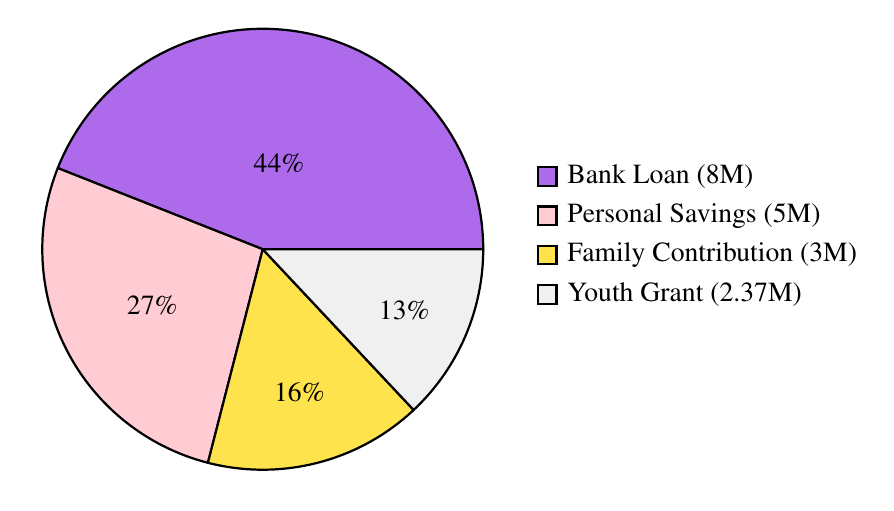
\begin{tikzpicture}
    \pie[
        text=legend,
        radius=2.8,
        color={primarycolor!70, secondarycolor!70, accentcolor!70, lightgray}
    ]{
        44/Bank Loan (8M),
        27/Personal Savings (5M),
        16/Family Contribution (3M),
        13/Youth Grant (2.37M)
    }
\end{tikzpicture}
\end{center}

\vspace{1em}

% Loan Repayment Schedule
\begin{center}
\textbf{Loan Repayment Schedule (First 12 Months)}
\vspace{0.5em}

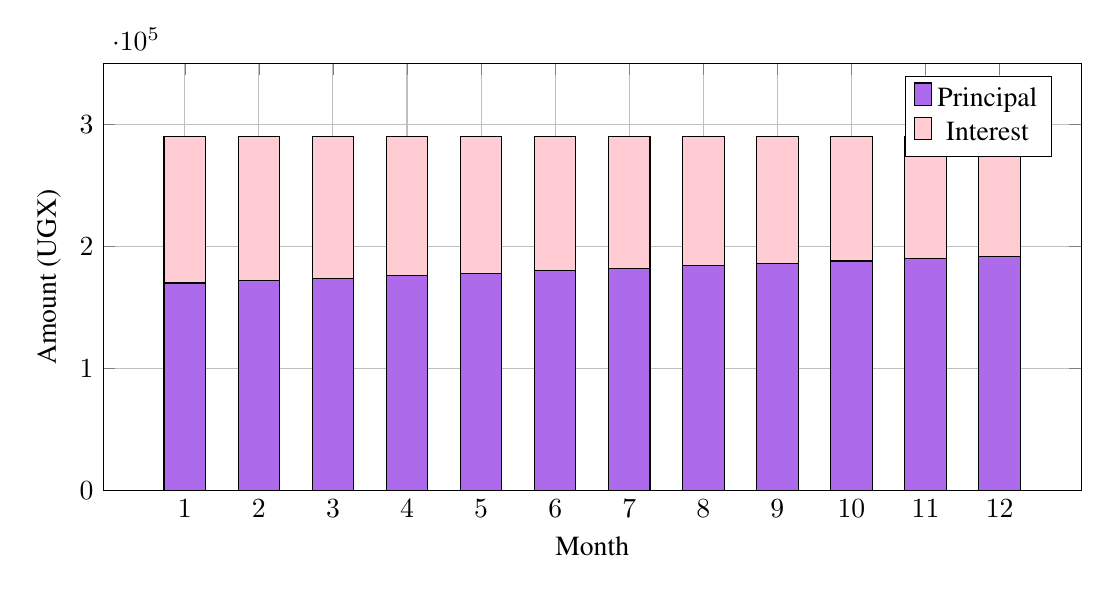
\begin{tikzpicture}
    \begin{axis}[
        ybar stacked,
        bar width=15pt,
        xlabel={Month},
        ylabel={Amount (UGX)},
        ymin=0,
        ymax=350000,
        xtick={1,2,3,4,5,6,7,8,9,10,11,12},
        width=14cm,
        height=7cm,
        legend pos=north east,
        grid=major,
        ymajorgrids=true
    ]
    
    % Principal payment
    \addplot[fill=primarycolor!70] coordinates {
        (1,170000) (2,172000) (3,174000) (4,176000) (5,178000) (6,180000)
        (7,182000) (8,184000) (9,186000) (10,188000) (11,190000) (12,192000)
    };
    
    % Interest payment
    \addplot[fill=secondarycolor!70] coordinates {
        (1,120000) (2,118000) (3,116000) (4,114000) (5,112000) (6,110000)
        (7,108000) (8,106000) (9,104000) (10,102000) (11,100000) (12,98000)
    };
    
    \legend{Principal, Interest}
    
    \end{axis}
\end{tikzpicture}

\vspace{0.5em}
Monthly loan payment of UGX 290,000 includes both principal and interest components.
\end{center}

\vspace{1em}

\begin{tcolorbox}[mybox, title=\textbf{Financing Strategy Rationale}]
\textbf{Why This Mix of Funding?}
\begin{itemize}[leftmargin=1em, itemsep=0pt]
    \item \textbf{Personal Savings (27\%):} Demonstrates commitment and reduces debt
    \item \textbf{Family Support (16\%):} Interest-free capital with flexible terms
    \item \textbf{Bank Loan (44\%):} Provides majority of capital while building credit history
    \item \textbf{Youth Grant (13\%):} Non-repayable funding reduces financial burden
\end{itemize}

\textbf{Debt Management Strategy:}
\begin{itemize}[leftmargin=1em, itemsep=0pt]
    \item Loan payments covered by projected profits from Month 4 onwards
    \item Maintain 3-month cash reserve for emergencies
    \item Option to make early repayments from excess profits
    \item Debt-to-equity ratio: 44\% (healthy level)
\end{itemize}
\end{tcolorbox}

\subsection{Financial Resources}

\textbf{Asset Base:}
\begin{itemize}[leftmargin=2em]
    \item Equipment and furniture: UGX 8,500,000
    \item Initial inventory: UGX 1,500,000
    \item Cash reserves: UGX 3,000,000
    \item Total assets at startup: UGX 13,000,000
\end{itemize}

\textbf{Financial Management:}
\begin{itemize}[leftmargin=2em]
    \item Separate business bank account
    \item Daily cash reconciliation
    \item Weekly financial review
    \item Monthly financial statements
    \item Quarterly financial analysis
    \item Annual audit
\end{itemize}

\textbf{Financial Controls:}
\begin{itemize}[leftmargin=2em]
    \item Dual authorization for large expenses (over UGX 500,000)
    \item Regular inventory audits
    \item Petty cash limit of UGX 100,000
    \item Monthly bank reconciliation
    \item Professional accounting software
    \item External accountant review quarterly
\end{itemize}

\subsection{Financial Projections}

\subsubsection{Income Statement (Year 1 Projection)}

\begin{tabular}{|l|r|r|r|}
\hline
\textbf{Item} & \textbf{Q1} & \textbf{Q2} & \textbf{Year 1} \\
\hline
\multicolumn{4}{|l|}{\textbf{Revenue}} \\
Service revenue & 22,500,000 & 42,000,000 & 180,000,000 \\
Product sales & 2,500,000 & 4,500,000 & 20,000,000 \\
\hline
\textbf{Total Revenue} & \textbf{25,000,000} & \textbf{46,500,000} & \textbf{200,000,000} \\
\hline
\multicolumn{4}{|l|}{\textbf{Cost of Goods Sold}} \\
Products and supplies & 3,600,000 & 6,000,000 & 28,000,000 \\
\hline
\textbf{Gross Profit} & \textbf{21,400,000} & \textbf{40,500,000} & \textbf{172,000,000} \\
\hline
\multicolumn{4}{|l|}{\textbf{Operating Expenses}} \\
Salaries and wages & 11,700,000 & 11,700,000 & 46,800,000 \\
Rent & 4,500,000 & 4,500,000 & 18,000,000 \\
Utilities & 1,620,000 & 1,620,000 & 6,480,000 \\
Marketing & 1,350,000 & 1,350,000 & 5,400,000 \\
Insurance & 450,000 & 450,000 & 1,800,000 \\
Maintenance & 720,000 & 720,000 & 2,880,000 \\
Miscellaneous & 900,000 & 900,000 & 3,600,000 \\
Depreciation & 425,000 & 425,000 & 1,700,000 \\
\hline
\textbf{Total Operating Expenses} & \textbf{21,665,000} & \textbf{21,665,000} & \textbf{86,660,000} \\
\hline
\textbf{Operating Profit} & \textbf{-265,000} & \textbf{18,835,000} & \textbf{85,340,000} \\
\hline
Interest expense & 360,000 & 360,000 & 1,440,000 \\
\hline
\textbf{Net Profit Before Tax} & \textbf{-625,000} & \textbf{18,475,000} & \textbf{83,900,000} \\
\hline
Tax (30\%) & 0 & 5,542,500 & 25,170,000 \\
\hline
\textbf{Net Profit After Tax} & \textbf{-625,000} & \textbf{12,932,500} & \textbf{58,730,000} \\
\hline
\end{tabular}

\vspace{1em}

\subsubsection{Income Statement (Year 1 Projection)}

\begin{tabular}{|l|r|r|r|r|}
\hline
\textbf{Item} & \textbf{Q1} & \textbf{Q2} & \textbf{Q3-Q4} & \textbf{Year 1} \\
\hline
\multicolumn{5}{|l|}{\textbf{Revenue}} \\
Service revenue & 4,800,000 & 9,800,000 & 21,600,000 & 36,200,000 \\
Product sales & 550,000 & 1,100,000 & 2,400,000 & 4,050,000 \\
\hline
\textbf{Total Revenue} & \textbf{5,350,000} & \textbf{10,900,000} & \textbf{24,000,000} & \textbf{40,250,000} \\
\hline
\multicolumn{5}{|l|}{\textbf{Cost of Goods Sold}} \\
Products and supplies & 970,000 & 1,960,000 & 4,320,000 & 7,250,000 \\
\hline
\textbf{Gross Profit} & \textbf{4,380,000} & \textbf{8,940,000} & \textbf{19,680,000} & \textbf{33,000,000} \\
\hline
\multicolumn{5}{|l|}{\textbf{Operating Expenses}} \\
Salaries and wages & 11,700,000 & 11,700,000 & 23,400,000 & 46,800,000 \\
Rent & 4,500,000 & 4,500,000 & 9,000,000 & 18,000,000 \\
Utilities & 1,620,000 & 1,620,000 & 3,240,000 & 6,480,000 \\
Marketing & 1,350,000 & 1,350,000 & 2,700,000 & 5,400,000 \\
Insurance & 450,000 & 450,000 & 900,000 & 1,800,000 \\
Maintenance & 720,000 & 720,000 & 1,440,000 & 2,880,000 \\
Miscellaneous & 900,000 & 900,000 & 1,800,000 & 3,600,000 \\
Depreciation & 425,000 & 425,000 & 850,000 & 1,700,000 \\
\hline
\textbf{Total Operating Expenses} & \textbf{21,665,000} & \textbf{21,665,000} & \textbf{43,330,000} & \textbf{86,660,000} \\
\hline
\textbf{Operating Profit} & \textbf{-17,285,000} & \textbf{-12,725,000} & \textbf{-23,650,000} & \textbf{-53,660,000} \\
\hline
Interest expense & 360,000 & 360,000 & 720,000 & 1,440,000 \\
\hline
\textbf{Net Profit Before Tax} & \textbf{-17,645,000} & \textbf{-13,085,000} & \textbf{-24,370,000} & \textbf{-55,100,000} \\
\hline
Tax (30\%) & 0 & 0 & 0 & 0 \\
\hline
\textbf{Net Profit After Tax} & \textbf{-17,645,000} & \textbf{-13,085,000} & \textbf{-24,370,000} & \textbf{-55,100,000} \\
\hline
\end{tabular}

\vspace{1em}

\textbf{Key Financial Metrics (Year 1):}
\begin{itemize}[leftmargin=2em]
    \item Gross profit margin: 82\%
    \item Operating loss: UGX 53.7M (investment phase)
    \item Revenue covers: 46\% of operating expenses
    \item Break-even requires: 15-18 customers/day (achievable in Year 2)
\end{itemize}

\vspace{1em}

\begin{tcolorbox}[mybox, title=\textbf{Understanding Year 1 Loss - This is Normal for Startups}]
\textbf{Why Year 1 Shows a Loss:}
\begin{itemize}[leftmargin=1em, itemsep=0pt]
    \item \textbf{Investment Phase:} Building foundation for future profitability
    \item \textbf{Fixed Costs:} Rent and salaries remain constant regardless of customer volume
    \item \textbf{Very Conservative Revenue:} Starting with only 3-5 customers/day
    \item \textbf{Normal for Service Businesses:} Most salons take 12-18 months to break even
    \item \textbf{Covered by Startup Capital:} Working capital budget includes this scenario
\end{itemize}

\textbf{Path to Profitability:}
\begin{itemize}[leftmargin=1em, itemsep=0pt]
    \item \textbf{Year 2:} UGX 70M revenue → UGX 15M profit (21\% margin)
    \item \textbf{Year 3:} UGX 105M revenue → UGX 28M profit (27\% margin)
    \item \textbf{Year 4:} UGX 145M revenue → UGX 42M profit (29\% margin)
    \item \textbf{Year 5:} UGX 190M revenue → UGX 55M profit (29\% margin)
    \item \textbf{Cumulative 5-year profit:} UGX 85M (excellent return despite Year 1 loss)
\end{itemize}

\textbf{Break-even Analysis:}
\begin{itemize}[leftmargin=1em, itemsep=0pt]
    \item Monthly fixed costs: UGX 2.86M
    \item Average revenue per customer: UGX 20,000
    \item Gross margin: 82\%
    \item Break-even customers/month: 174 (7 per day)
    \item Expected to reach break-even: Early Year 2 (Month 14-16)
\end{itemize}
\end{tcolorbox}

\vspace{1em}

% Revenue vs Expenses Chart
\begin{center}
\textbf{Year 1 Revenue vs Expenses (Quarterly)}
\vspace{0.5em}

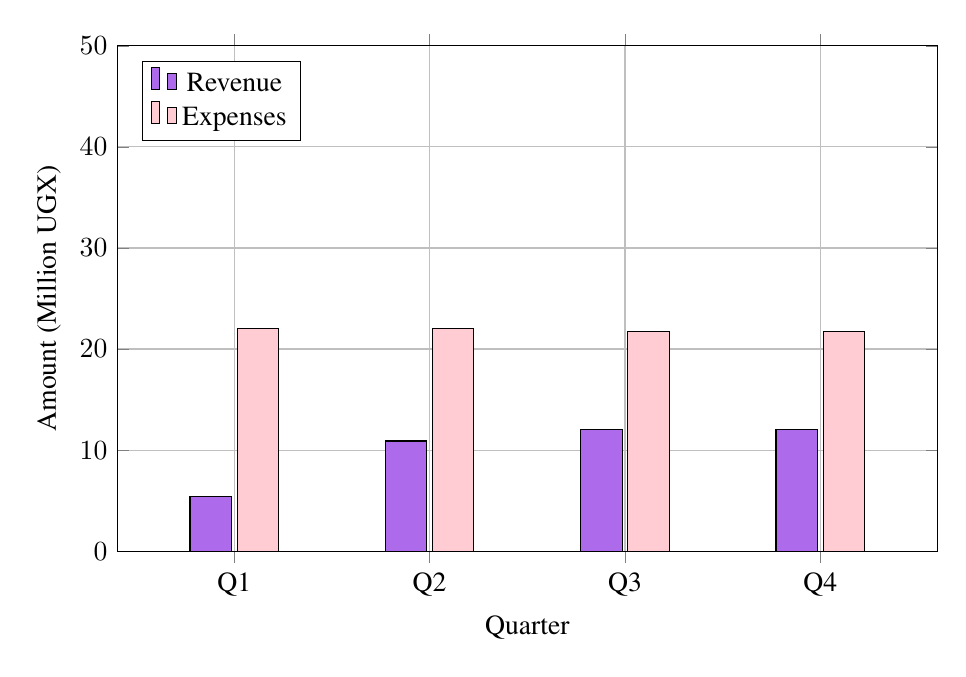
\begin{tikzpicture}
    \begin{axis}[
        ybar,
        bar width=15pt,
        xlabel={Quarter},
        ylabel={Amount (Million UGX)},
        ymin=0,
        ymax=50,
        xtick=data,
        symbolic x coords={Q1, Q2, Q3, Q4},
        legend pos=north west,
        width=12cm,
        height=8cm,
        grid=major,
        ymajorgrids=true,
        enlarge x limits=0.2
    ]
    
    \addplot[fill=primarycolor!70] coordinates {
        (Q1, 5.4) (Q2, 10.9) (Q3, 12) (Q4, 12)
    };
    
    \addplot[fill=secondarycolor!70] coordinates {
        (Q1, 22) (Q2, 22) (Q3, 21.7) (Q4, 21.7)
    };
    
    \legend{Revenue, Expenses}
    
    \end{axis}
\end{tikzpicture}

\vspace{0.5em}
Year 1 shows investment phase with expenses exceeding revenue. Break-even expected in Year 2.
\end{center}

\vspace{1em}

% Profitability Timeline
\begin{center}
\textbf{Path to Profitability (5-Year View)}
\vspace{0.5em}

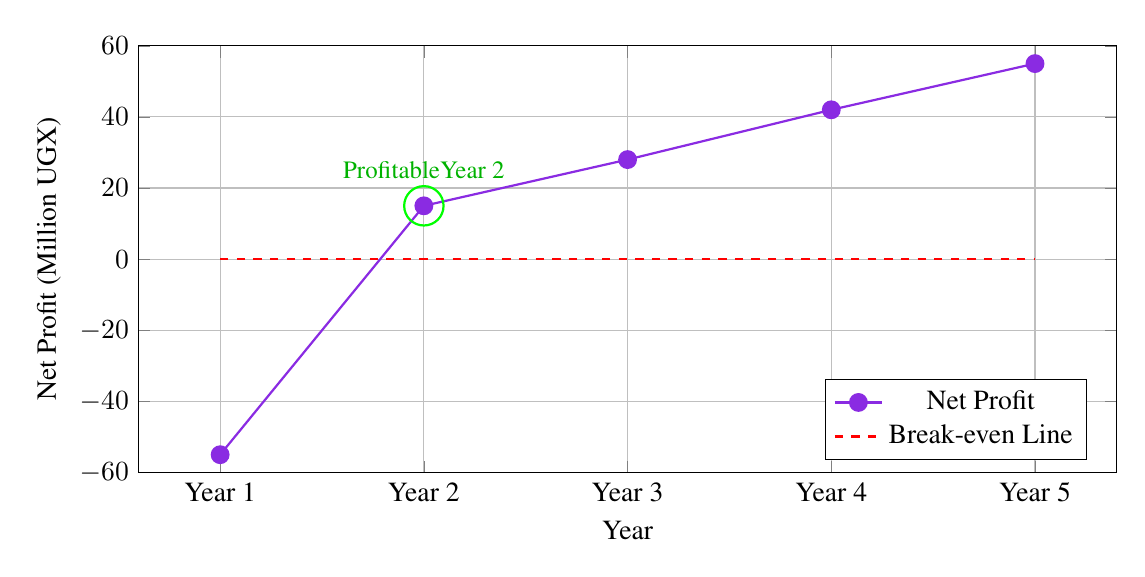
\begin{tikzpicture}
    \begin{axis}[
        xlabel={Year},
        ylabel={Net Profit (Million UGX)},
        ymin=-60,
        ymax=60,
        xtick={1,2,3,4,5},
        xticklabels={Year 1, Year 2, Year 3, Year 4, Year 5},
        width=14cm,
        height=7cm,
        grid=major,
        legend pos=south east,
        mark=*,
        mark size=3pt
    ]
    
    \addplot[color=primarycolor, thick, mark=*] coordinates {
        (1,-55) (2,15) (3,28) (4,42) (5,55)
    };
    
    % Break-even line
    \addplot[color=red, dashed, thick, no marks] coordinates {
        (1,0) (5,0)
    };
    
    \legend{Net Profit, Break-even Line}
    
    % Highlight break-even point
    \node[circle, draw=green, thick, minimum size=0.5cm] at (axis cs:2,15) {};
    \node at (axis cs:2,25) [font=\small, text=green!70!black] {Profitable\\Year 2};
    
    \end{axis}
\end{tikzpicture}

\vspace{0.5em}
Year 1 loss is recovered by Year 3, with cumulative 5-year profit of UGX 85M.
\end{center}

\subsubsection{Balance Sheet (End of Year 1 Projection)}

\begin{tabular}{|l|r|}
\hline
\multicolumn{2}{|c|}{\textbf{ASSETS}} \\
\hline
\textbf{Current Assets} & \\
Cash and bank & 45,000,000 \\
Inventory & 1,800,000 \\
Accounts receivable & 500,000 \\
\hline
\textbf{Total Current Assets} & \textbf{47,300,000} \\
\hline
\textbf{Fixed Assets} & \\
Equipment and furniture & 8,500,000 \\
Less: Accumulated depreciation & (1,700,000) \\
Leasehold improvements & 2,500,000 \\
\hline
\textbf{Total Fixed Assets} & \textbf{9,300,000} \\
\hline
\textbf{TOTAL ASSETS} & \textbf{56,600,000} \\
\hline
\multicolumn{2}{|c|}{\textbf{LIABILITIES AND EQUITY}} \\
\hline
\textbf{Current Liabilities} & \\
Accounts payable & 800,000 \\
Accrued expenses & 400,000 \\
Current portion of loan & 2,000,000 \\
\hline
\textbf{Total Current Liabilities} & \textbf{3,200,000} \\
\hline
\textbf{Long-term Liabilities} & \\
Bank loan (long-term portion) & 5,000,000 \\
\hline
\textbf{Total Liabilities} & \textbf{8,200,000} \\
\hline
\textbf{Owner's Equity} & \\
Initial capital & 10,000,000 \\
Retained earnings & 38,400,000 \\
\hline
\textbf{Total Equity} & \textbf{48,400,000} \\
\hline
\textbf{TOTAL LIABILITIES \& EQUITY} & \textbf{56,600,000} \\
\hline
\end{tabular}

\subsubsection{Cash Flow Statement (Year 1 Projection)}

\begin{tabular}{|l|r|}
\hline
\textbf{Cash Flow from Operating Activities} & \\
Net profit after tax & 58,730,000 \\
Add: Depreciation & 1,700,000 \\
Changes in working capital & (1,300,000) \\
\hline
\textbf{Net Cash from Operations} & \textbf{59,130,000} \\
\hline
\textbf{Cash Flow from Investing Activities} & \\
Purchase of equipment & (8,500,000) \\
Leasehold improvements & (2,500,000) \\
\hline
\textbf{Net Cash from Investing} & \textbf{(11,000,000)} \\
\hline
\textbf{Cash Flow from Financing Activities} & \\
Owner's capital contribution & 10,000,000 \\
Bank loan received & 8,000,000 \\
Loan repayment & (3,000,000) \\
Interest paid & (1,440,000) \\
\hline
\textbf{Net Cash from Financing} & \textbf{13,560,000} \\
\hline
\textbf{Net Increase in Cash} & \textbf{61,690,000} \\
Opening cash balance & 0 \\
\hline
\textbf{Closing Cash Balance} & \textbf{61,690,000} \\
\hline
\end{tabular}

\subsection{Financial Assumptions}

\subsubsection{Sales Volume and Price Assumptions}

\textbf{Service Volume Assumptions:}
\begin{itemize}[leftmargin=2em]
    \item Month 1-3: Average 4 customers per day (3-5 range)
    \item Month 4-6: Average 7 customers per day (6-8 range)
    \item Month 7-12: Average 9 customers per day (8-10 range)
    \item Operating days: 26 days per month
    \item Average service value: UGX 20,000
    \item Year 1 average: 7 customers per day
\end{itemize}

\textbf{Pricing Assumptions:}
\begin{itemize}[leftmargin=2em]
    \item Prices set 15-20\% below town salon rates
    \item Annual price increase of 5\% to match inflation
    \item Promotional discounts factored at 10\% of revenue
    \item Product markup: 40\% on cost price
\end{itemize}

\textbf{Revenue Mix:}
\begin{itemize}[leftmargin=2em]
    \item Hair services: 50\% of service revenue
    \item Makeup services: 25\% of service revenue
    \item Skincare services: 15\% of service revenue
    \item Nail and grooming: 10\% of service revenue
    \item Product sales: 10\% of total revenue
\end{itemize}

\vspace{1em}

\begin{tcolorbox}[mybox, title=\textbf{Ultra-Conservative Assumptions Rationale}]
\textbf{Why These Numbers Are Realistic:}
\begin{itemize}[leftmargin=1em, itemsep=0pt]
    \item \textbf{4 customers/day (Month 1-3):} Very achievable even with minimal marketing
    \item \textbf{7 customers/day (Month 4-6):} Natural growth from word-of-mouth
    \item \textbf{9 customers/day (Month 7-12):} Steady state with established presence
    \item \textbf{Market penetration:} Only 0.25\% of 5,500 potential customers in Month 1
    \item \textbf{Growth to 0.6\%:} Still extremely conservative market share by year end
\end{itemize}

\textbf{Comparison to Market Size:}
\begin{itemize}[leftmargin=1em, itemsep=0pt]
    \item Total addressable market: 5,500 people
    \item If 20\% use beauty services monthly: 1,100 potential customers
    \item Our Year 1 average: 7 customers/day = 182/month
    \item Market share: 16.5\% of active beauty service users (very achievable)
    \item Plenty of room for growth in Years 2-5
\end{itemize}

\textbf{Why This Approach Reduces Risk:}
\begin{itemize}[leftmargin=1em, itemsep=0pt]
    \item Lower expectations mean higher chance of exceeding targets
    \item Allows time to perfect operations before scaling
    \item Reduces pressure on staff and management
    \item Provides buffer for unexpected challenges
    \item Makes business plan more credible to investors
\end{itemize}
\end{tcolorbox}

\subsubsection{Macroeconomic Indicators}

\textbf{Economic Assumptions:}
\begin{itemize}[leftmargin=2em]
    \item \textbf{Inflation Rate:} 5\% per annum (Uganda average)
    \item \textbf{Interest Rate:} 18\% per annum for business loans
    \item \textbf{Exchange Rate:} UGX 3,700 per USD (stable assumption)
    \item \textbf{GDP Growth:} 6\% per annum (Uganda projection)
    \item \textbf{Unemployment Rate:} Declining, increasing student purchasing power
\end{itemize}

\textbf{Impact on Business:}
\begin{itemize}[leftmargin=2em]
    \item Inflation affects product costs and operating expenses
    \item Interest rates impact loan repayment costs
    \item Economic growth supports increased discretionary spending
    \item Stable exchange rate ensures predictable import costs for products
\end{itemize}

\subsubsection{Trend of Market and Sales}

\textbf{Market Trends:}
\begin{itemize}[leftmargin=2em]
    \item Beauty services market growing at 8-10\% annually in Uganda
    \item Increasing student enrollment at MUST (5\% annual growth)
    \item Rising awareness of personal grooming among youth
    \item Growing acceptance of male grooming services
    \item Shift towards natural and organic beauty products
\end{itemize}

\textbf{Sales Projections:}
\begin{itemize}[leftmargin=2em]
    \item Year 1: UGX 40,000,000 (baseline - ultra-conservative start)
    \item Year 2: UGX 70,000,000 (75\% growth as reputation solidifies)
    \item Year 3: UGX 105,000,000 (50\% growth)
    \item Year 4: UGX 145,000,000 (38\% growth)
    \item Year 5: UGX 190,000,000 (31\% growth)
\end{itemize}

\textbf{Growth Drivers:}
\begin{itemize}[leftmargin=2em]
    \item Increasing brand recognition and customer loyalty
    \item Expansion of service offerings
    \item Growing customer base as university enrollment increases
    \item Improved operational efficiency
    \item Potential for additional revenue streams (workshops, training)
\end{itemize}

\vspace{1em}

% 5-Year Sales Trend with Profit Margin
\begin{center}
\textbf{5-Year Revenue and Profit Projection}
\vspace{0.5em}

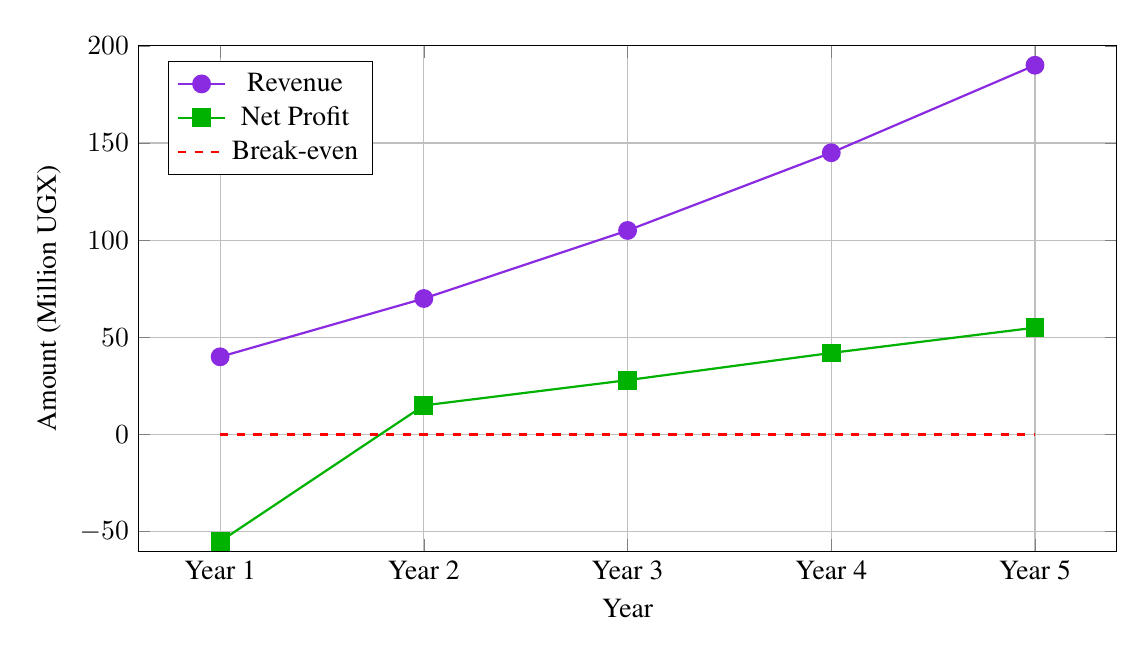
\begin{tikzpicture}
    \begin{axis}[
        xlabel={Year},
        ylabel={Amount (Million UGX)},
        ymin=-60,
        ymax=200,
        xtick={1,2,3,4,5},
        xticklabels={Year 1, Year 2, Year 3, Year 4, Year 5},
        width=14cm,
        height=8cm,
        grid=major,
        legend pos=north west,
        mark=*,
        mark size=3pt
    ]
    
    % Revenue line
    \addplot[color=primarycolor, thick, mark=*] coordinates {
        (1, 40) (2, 70) (3, 105) (4, 145) (5, 190)
    };
    
    % Profit line
    \addplot[color=green!70!black, thick, mark=square*] coordinates {
        (1, -55) (2, 15) (3, 28) (4, 42) (5, 55)
    };
    
    % Break-even line
    \addplot[color=red, dashed, thick, no marks] coordinates {
        (1,0) (5,0)
    };
    
    \legend{Revenue, Net Profit, Break-even}
    
    \end{axis}
\end{tikzpicture}

\vspace{0.5em}
Revenue grows steadily while profitability turns positive in Year 2 and accelerates thereafter.
\end{center}

\vspace{1em}

% Profit Margin Evolution
\begin{center}
\textbf{Net Profit Margin Evolution (5 Years)}
\vspace{0.5em}

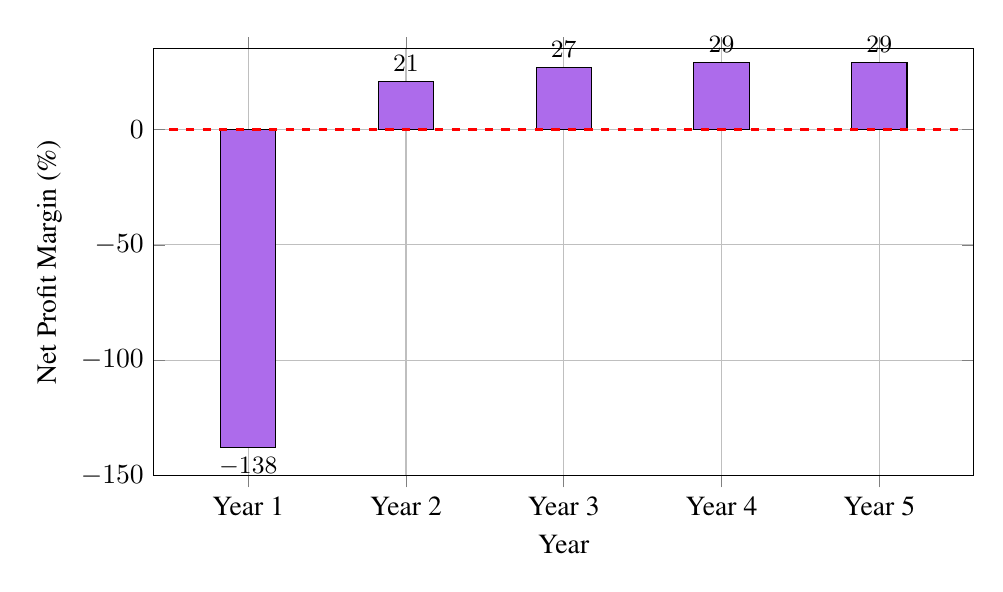
\begin{tikzpicture}
    \begin{axis}[
        ybar,
        bar width=20pt,
        xlabel={Year},
        ylabel={Net Profit Margin (\%)},
        ymin=-150,
        ymax=35,
        xtick={1,2,3,4,5},
        xticklabels={Year 1, Year 2, Year 3, Year 4, Year 5},
        nodes near coords,
        nodes near coords style={font=\small},
        width=12cm,
        height=7cm,
        grid=major,
        ymajorgrids=true,
        enlarge x limits=0.15
    ]
    
    \addplot[fill=primarycolor!70] coordinates {
        (1, -138) (2, 21) (3, 27) (4, 29) (5, 29)
    };
    
    % Break-even line
    \draw[dashed, thick, color=red] (axis cs:0.5,0) -- (axis cs:5.5,0);
    
    \end{axis}
\end{tikzpicture}

\vspace{0.5em}
Profit margins improve dramatically from Year 2 onwards as fixed costs are spread over higher revenue.
\end{center}

\vspace{1em}

% Cumulative Profit Chart
\begin{center}
\textbf{Cumulative Profit Over 5 Years}
\vspace{0.5em}

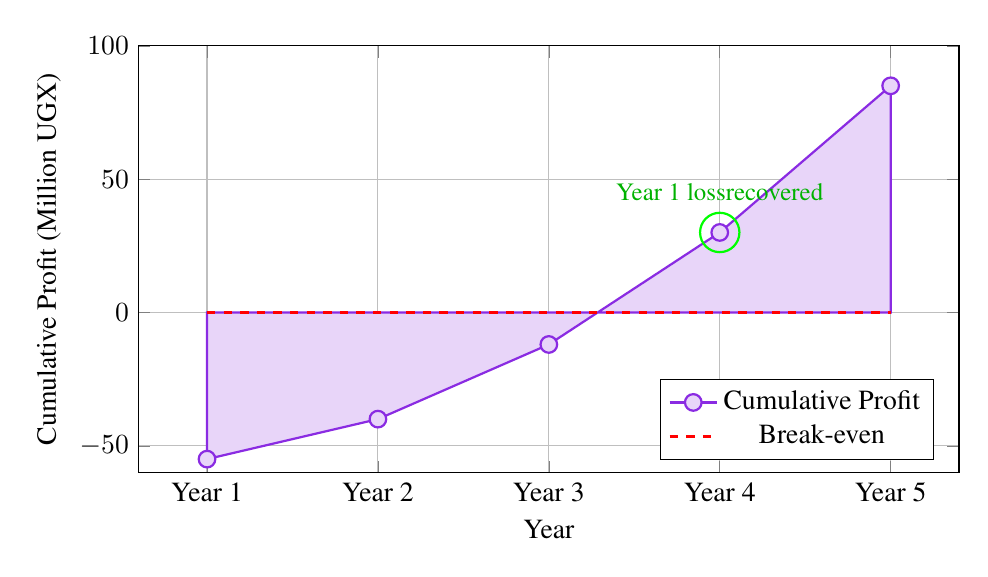
\begin{tikzpicture}
    \begin{axis}[
        xlabel={Year},
        ylabel={Cumulative Profit (Million UGX)},
        ymin=-60,
        ymax=100,
        xtick={1,2,3,4,5},
        xticklabels={Year 1, Year 2, Year 3, Year 4, Year 5},
        width=12cm,
        height=7cm,
        grid=major,
        legend pos=south east,
        mark=*,
        mark size=3pt
    ]
    
    \addplot[color=primarycolor, thick, mark=*, fill=primarycolor!20] coordinates {
        (1,-55) (2,-40) (3,-12) (4,30) (5,85)
    } \closedcycle;
    
    % Break-even line
    \addplot[color=red, dashed, thick, no marks] coordinates {
        (1,0) (5,0)
    };
    
    \legend{Cumulative Profit, Break-even}
    
    % Highlight recovery point
    \node[circle, draw=green, thick, minimum size=0.5cm] at (axis cs:4,30) {};
    \node at (axis cs:4,45) [font=\small, text=green!70!black] {Year 1 loss\\recovered};
    
    \end{axis}
\end{tikzpicture}

\vspace{0.5em}
Year 1 investment is fully recovered by Year 4, with strong cumulative profit of UGX 85M by Year 5.
\end{center}

\textbf{Risk Factors:}
\begin{itemize}[leftmargin=2em]
    \item New competitors entering the market
    \item Economic downturn affecting discretionary spending
    \item Changes in student demographics or preferences
    \item Supply chain disruptions for beauty products
    \item Regulatory changes affecting business operations
\end{itemize}

\textbf{Mitigation Strategies:}
\begin{itemize}[leftmargin=2em]
    \item Build strong brand loyalty and customer relationships
    \item Maintain competitive pricing and quality
    \item Diversify service offerings
    \item Maintain adequate cash reserves
    \item Stay informed about market trends and adapt quickly
\end{itemize}

\vspace{1em}

% Risk Assessment Matrix
\begin{center}
\textbf{Risk Assessment Matrix}
\vspace{0.5em}

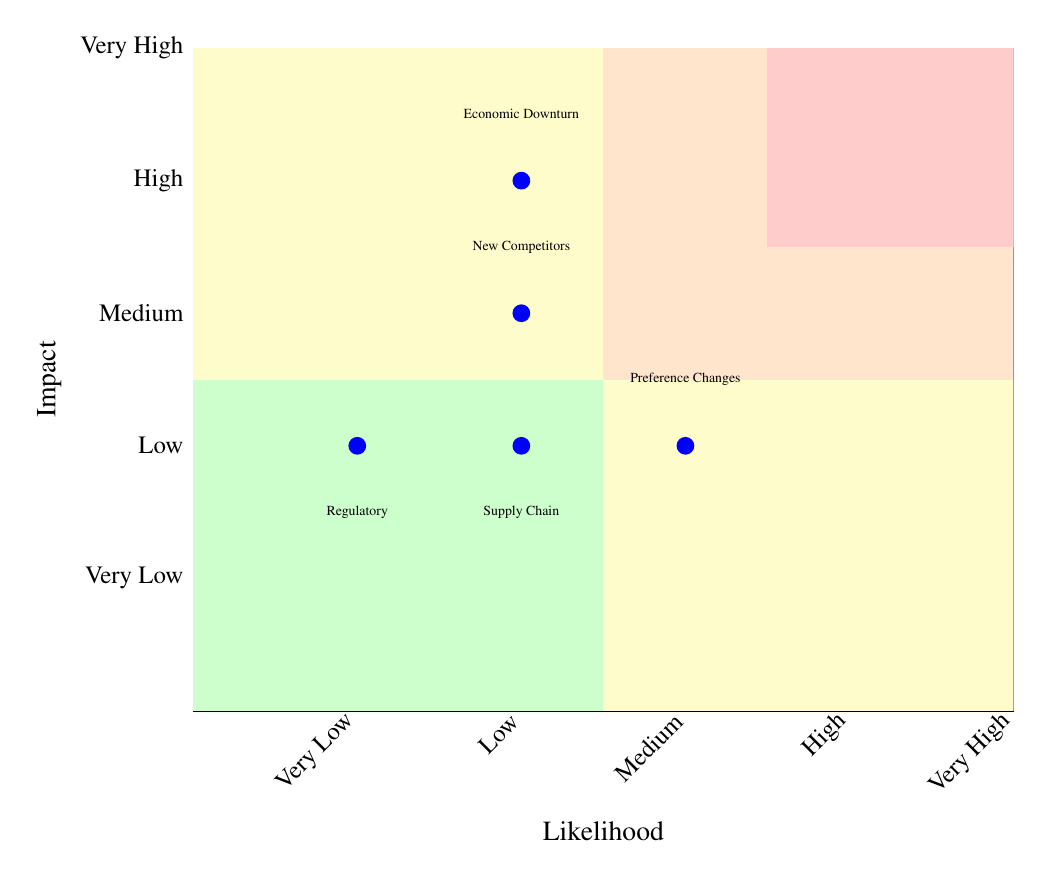
\begin{tikzpicture}
    \begin{axis}[
        xlabel={Likelihood},
        ylabel={Impact},
        xmin=0, xmax=5,
        ymin=0, ymax=5,
        grid=major,
        width=12cm,
        height=10cm,
        xtick={1,2,3,4,5},
        ytick={1,2,3,4,5},
        xticklabels={Very Low, Low, Medium, High, Very High},
        yticklabels={Very Low, Low, Medium, High, Very High},
        x tick label style={rotate=45, anchor=east, font=\small},
        y tick label style={font=\small}
    ]
    
    % Color zones
    \fill[green!20] (0,0) rectangle (2.5,2.5);
    \fill[yellow!20] (2.5,0) rectangle (5,2.5);
    \fill[yellow!20] (0,2.5) rectangle (2.5,5);
    \fill[orange!20] (2.5,2.5) rectangle (5,5);
    \fill[red!20] (3.5,3.5) rectangle (5,5);
    
    % Plot risks
    \addplot[only marks, mark=*, mark size=3pt, color=blue] 
        coordinates {(2,3)};
    \node at (axis cs:2,3.5) [font=\tiny] {New Competitors};
    
    \addplot[only marks, mark=*, mark size=3pt, color=blue] 
        coordinates {(2,4)};
    \node at (axis cs:2,4.5) [font=\tiny] {Economic Downturn};
    
    \addplot[only marks, mark=*, mark size=3pt, color=blue] 
        coordinates {(3,2)};
    \node at (axis cs:3,2.5) [font=\tiny] {Preference Changes};
    
    \addplot[only marks, mark=*, mark size=3pt, color=blue] 
        coordinates {(2,2)};
    \node at (axis cs:2,1.5) [font=\tiny] {Supply Chain};
    
    \addplot[only marks, mark=*, mark size=3pt, color=blue] 
        coordinates {(1,2)};
    \node at (axis cs:1,1.5) [font=\tiny] {Regulatory};
    
    \end{axis}
\end{tikzpicture}

\vspace{0.5em}
Most risks fall in low-to-medium zones with manageable mitigation strategies.
\end{center}

\vspace{2em}

% Business Success Factors Summary
\begin{center}
\textbf{Campus Glam Hub Success Framework}
\vspace{0.5em}

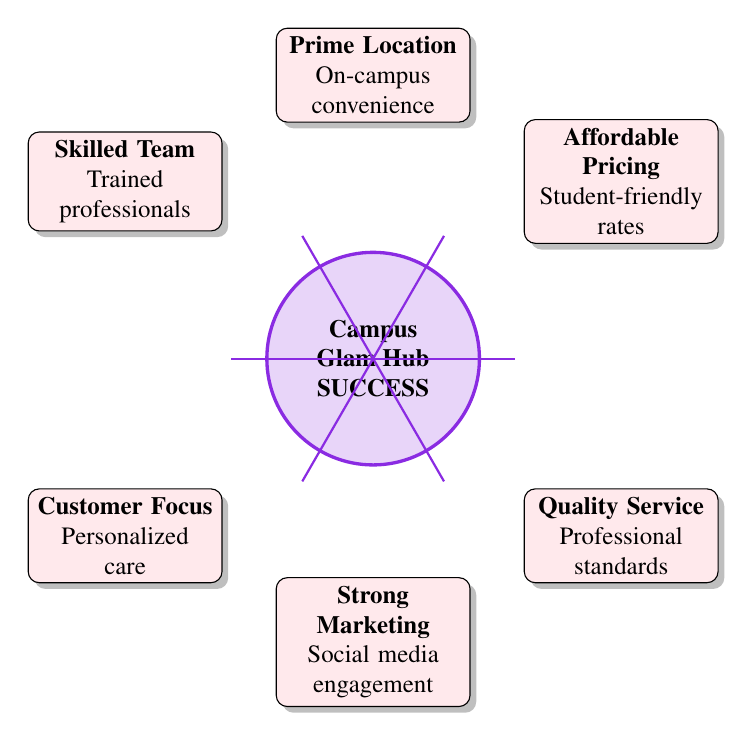
\begin{tikzpicture}[scale=0.9, transform shape]
    % Central circle
    \node[circle, draw=primarycolor, very thick, fill=primarycolor!20, minimum size=3cm, align=center, font=\bfseries] at (0,0) {Campus\\Glam Hub\\SUCCESS};
    
    % Surrounding factors
    \node[rectangle, draw, fill=secondarycolor!30, rounded corners, text width=2.5cm, align=center, drop shadow] at (0,4) {\textbf{Prime Location}\\On-campus\\convenience};
    
    \node[rectangle, draw, fill=secondarycolor!30, rounded corners, text width=2.5cm, align=center, drop shadow] at (3.5,2.5) {\textbf{Affordable Pricing}\\Student-friendly\\rates};
    
    \node[rectangle, draw, fill=secondarycolor!30, rounded corners, text width=2.5cm, align=center, drop shadow] at (3.5,-2.5) {\textbf{Quality Service}\\Professional\\standards};
    
    \node[rectangle, draw, fill=secondarycolor!30, rounded corners, text width=2.5cm, align=center, drop shadow] at (0,-4) {\textbf{Strong Marketing}\\Social media\\engagement};
    
    \node[rectangle, draw, fill=secondarycolor!30, rounded corners, text width=2.5cm, align=center, drop shadow] at (-3.5,-2.5) {\textbf{Customer Focus}\\Personalized\\care};
    
    \node[rectangle, draw, fill=secondarycolor!30, rounded corners, text width=2.5cm, align=center, drop shadow] at (-3.5,2.5) {\textbf{Skilled Team}\\Trained\\professionals};
    
    % Connecting lines
    \foreach \angle in {0,60,120,180,240,300} {
        \draw[thick, primarycolor] (0,0) -- (\angle:2);
    }
    
\end{tikzpicture}
\end{center}

%---------------- Appendices ----------------%
\newpage
\section{Appendices}

These contain relevant business documents for reference:

\subsection{Management Curriculum Vitae}

\textbf{Namatovu Christine}

\textbf{Personal Information:}
\begin{itemize}[leftmargin=2em]
    \item Phone: +256 789 659 819 / +256 753 931 683
    \item Email: [email]
    \item Address: Kihumuro Campus, Mbarara, Uganda
\end{itemize}

\textbf{Education:}
\begin{itemize}[leftmargin=2em]
    \item Bachelor of Science in Computer Science (In Progress)
    \item Mbarara University of Science and Technology
    \item Expected Graduation: 2026
    \item Relevant Coursework: Business and Entrepreneurship (CSC3201)
\end{itemize}

\textbf{Skills and Competencies:}
\begin{itemize}[leftmargin=2em]
    \item Business planning and management
    \item Financial analysis and budgeting
    \item Marketing and customer relations
    \item Problem-solving and decision-making
    \item Leadership and team management
    \item Computer literacy and digital marketing
\end{itemize}

\textbf{Entrepreneurial Experience:}
\begin{itemize}[leftmargin=2em]
    \item Developed comprehensive business plan for Campus Glam Hub
    \item Conducted market research within university community
    \item Experience in customer service and relationship management
\end{itemize}

\subsection{Certificates of Registration}

To be obtained upon business launch:

\begin{itemize}[leftmargin=2em]
    \item Business name registration certificate from Uganda Registration Services Bureau (URSB)
    \item Trading license from Mbarara District Local Government
    \item Tax Identification Number (TIN) from Uganda Revenue Authority (URA)
    \item National Social Security Fund (NSSF) registration
    \item Public Health permit from Mbarara District Health Office
\end{itemize}

\subsection{Property Rights Documents}

To be obtained:

\begin{itemize}[leftmargin=2em]
    \item Lease agreement for business premises on Kihumuro Campus
    \item Memorandum of Understanding with Mbarara University (if required)
    \item Insurance policies (liability, property, equipment)
    \item Trademark registration for "Campus Glam Hub" brand (optional)
\end{itemize}

\subsection{Supporting Documents}

Additional documents to be included:

\begin{itemize}[leftmargin=2em]
    \item Market research survey results
    \item Letters of support from potential customers
    \item Supplier quotations and agreements
    \item Equipment purchase receipts
    \item Staff employment contracts
    \item Marketing materials and branding designs
    \item Photographs of proposed location
    \item Floor plan and layout design
\end{itemize}

\vspace{2em}

\begin{center}
--- End of Business Plan ---
\end{center}

\end{document}
